\documentclass[10pt]{article}

% basic packages
\usepackage[margin=1in]{geometry}
\usepackage{fix-cm}        % scale one design size, as OT1 does --- keeps the title bold
\usepackage[T1]{fontenc}   % accented French terms kept inline in the prose
\usepackage[pdftex]{graphicx}
\graphicspath{{./src/}}
\usepackage{amsmath,amssymb,amsthm}
\usepackage{custom}
\usepackage{pdfpages}
\usepackage{subcaption}
\usepackage{tabularx}
\usepackage{xcolor}

\usepackage{pgfplots}
\pgfplotsset{compat=1.15}
\usetikzlibrary{arrows,calc,decorations.markings,patterns}

\renewcommand\qedsymbol{$\blacksquare$}

% page formatting
\usepackage{fancyhdr}
\pagestyle{fancy}

\usepackage{titlesec}
\titleformat*{\subsubsection}{\large\bfseries\sffamily}

\renewcommand{\sectionmark}[1]{\markright{\textsf{\arabic{section}. #1}}}
\renewcommand{\subsectionmark}[1]{}
\lhead{\textbf{\thepage} \ \ \nouppercase{\rightmark}}
\chead{}
\rhead{}
\lfoot{}
\cfoot{}
\rfoot{}
\setlength{\headheight}{14pt}

\linespread{1.03} % give a little extra room
\setlength{\parindent}{0in} % reduce paragraph indent a bit
\setcounter{secnumdepth}{2} % no numbered subsubsections
\setcounter{tocdepth}{2} % no subsubsections in ToC

\begin{document}

% make title page
\thispagestyle{empty}
\bigskip \
\vspace{0.1cm}

\begin{center}
{\fontsize{30}{30} \selectfont \bf \sffamily ECE 3TC21: Propagation et Antennes }\\
\vspace{24pt}
%{\fontsize{14}{14} \selectfont \rmfamily Donald Kong} \\
%\vspace{6pt}
%{\fontsize{12}{12} \selectfont \ttfamily dkkl1137@gmail.com} \\
%\vspace{24pt}
\end{center}

{\parindent0pt \baselineskip=15.5pt
  Antennes \& propagation dans les systèmes radiofréquences. The module
  covers what a radio link is made of and why it is engineered the way it is:
  the plane monochromatic wave in a linear, homogeneous, isotropic medium and
  the Maxwell equations behind it; transmission-line theory, from the
  telegrapher's equations to characteristic impedance, the reflection
  coefficient and standing waves; impedance matching by quarter-wave
  transformer, stub and lumped elements, and the scattering parameters that
  describe a matched network at RF; antennas --- input impedance, radiation
  pattern, directivity, gain, polarisation --- and the usual families, wire,
  aperture, reflector, printed and array; and finally the link budget, the
  Friis equation and the atmospheric and terrain effects that degrade it.

  \medskip
  Prose is in English; the French terms the poly, the TDs and the exam actually
  use are kept inline, so the vocabulary stays findable in both languages.
}

% make table of contents
% \newpage
\microtoc%
\newpage

% main content
\section{Les systèmes de télécommunications sans fil}
Si la dénomination de « \textbf{systèmes de télécommunications} »
(\textit{telecommunication systems}) paraît quelque peu abstraite, elle englobe
en réalité un grand nombre d'objets et équipements qui nous sont très familiers.
This first part fixes what such a system is, what all of them have in common,
why they are operated at radio frequencies rather than at the audio frequencies
of a first electronics course, and what makes radio-frequency engineering a
different discipline from electronics at basse fréquence. It ends on the single
problem that organises the whole module: a signal radiofréquence loses power
everywhere it goes, and the two engineering answers to that are amplification
and adaptation d'impédance.

\subsection{Systèmes de télécommunications}

\begin{definition}[Système de télécommunications]
  Les \textbf{systèmes de télécommunications} émettent et reçoivent de
  l'information (voix, vidéo, fichiers, données en streaming) grâce à des
  ondes électromagnétiques qui sont rayonnées et captées par des antennes. Ils
  contiennent des circuits électroniques émetteurs et récepteurs.
\end{definition}

The course splits the field by market volume rather than by physics, because the
volume drives the engineering constraints.

\paragraph{Applications grand public} Les systèmes de télécommunications sont
pour la plupart des objets que nous utilisons au quotidien : smartphones,
tablettes, boxes internet, systèmes de navigation GPS (\textit{Global
Positioning System}), oreillettes Bluetooth, montres connectées, radars d'aide à
la conduite automobile, antenne parabolique et \textbf{démodulateur}
(\textit{demodulator}) pour réception de TV par satellite. Tous ces appareils
sont utilisés dans des \textbf{applications grand public} (\textit{consumer
applications}) : volume de ventes très important, chiffrés en millions ou
milliards d'unités.

\paragraph{Applications spécialisées} En plus des applications grand public, il
existe également des systèmes de télécommunications dédiés à des applications
dites spécialisées (volume de ventes très modeste, chiffré en centaines voire
dizaines d'unités). Il s'agit des satellites en orbite autour de la Terre, qui
permettent les prévisions météorologiques, la réception de TV par satellite, la
radioastronomie, l'observation de l'évolution de la déforestation ou la fonte
des glaces. Un autre type d'application spécialisée concerne les activités
militaires et de défense : radars de détection et surveillance, systèmes
d'armement, de \textbf{brouillage} (\textit{jamming}), de guidage de missiles,
communications militaires sécurisées.

\begin{remark}
  Les antennes utilisées dans ces applications se différencient par leur forme,
  leur taille, leurs performances et caractéristiques techniques. There is no
  universal antenne: il existe toutes sortes d'antennes répondant chacune à des
  contraintes particulières en fonction des applications visées. The module
  later surveys antennes filaires, antennes à ouverture rayonnante, antennes à
  réflecteur, antennes planaires and antennes réseaux for exactly that reason.
\end{remark}

\subsection{Quelles sont les caractéristiques des systèmes de télécommunications ?}
Comme nous venons de le voir, les systèmes de télécommunications sont utilisés
dans des applications très différentes et cependant, ils possèdent 3 points
communs.

\paragraph{1. Ils rayonnent et captent des ondes électromagnétiques}
Les systèmes de télécommunications émettent et reçoivent de l'information grâce
à des \textbf{ondes électromagnétiques} (\textit{electromagnetic wave}, OEM) qui
sont rayonnées en \textbf{émission}
(\textit{transmission}) et captées en réception par des antennes.
In the canonical picture --- une communication entre un smartphone émettant une
onde électromagnétique et une \textbf{station de base} (\textit{base station},
BTS, \textit{Base Transceiver Station}) recevant cette onde --- les champs
électrique $E$ et magnétique $H$ sont orthogonaux entre eux et orthogonaux à
la direction de propagation (définie par le vecteur d'onde) de l'onde.

\begin{definition}[Longueur d'onde]
  La \textbf{longueur d'onde} (\textit{wavelength}) $\lambda$ est la fréquence
  spatiale de l'onde électromagnétique. Avec $f$ la fréquence du signal et $c$
  la vitesse de la lumière,
  \[\lambda=\frac{c}{f},\qquad c \simeq 3\times 10^{8}\ \text{m/s}.\]
\end{definition}

Propagation libre ou guidée d'une onde électromagnétique : \textit{libre} in
\textbf{espace libre} (\textit{free space}), \textit{guidée} in a ligne de
transmission or a cable, which is \textbf{propagation guidée} (\textit{guided propagation}). Both
cases are governed by the same équations de Maxwell. Un rappel des notions de
base en électromagnétisme sera fait dans la deuxième partie.

\paragraph{2. Les ondes sont des signaux radiofréquence}
\begin{definition}[Signal radiofréquence]
  Les ondes électromagnétiques utilisées par les systèmes de télécommunications
  sont des \textbf{signaux radiofréquence} (\textit{radio-frequency signal},
  RF), c'est-à-dire des signaux dont
  la fréquence est approximativement comprise entre $100$ MHz et $100$ GHz.
\end{definition}

Ces fréquences sont donc très élevées… en tout cas bien plus élevées que les
fréquences que vous avez utilisées en cours d'électronique
($1$ kHz\,--\,$100$ kHz) jusqu'à présent. La figure ci-dessous présente les
bandes de fréquences RF utilisées par les systèmes de télécommunications : c'est
le \textbf{spectre radiofréquence} (\textit{radio-frequency spectrum}).

\begin{figure}[h!]
  \centering
  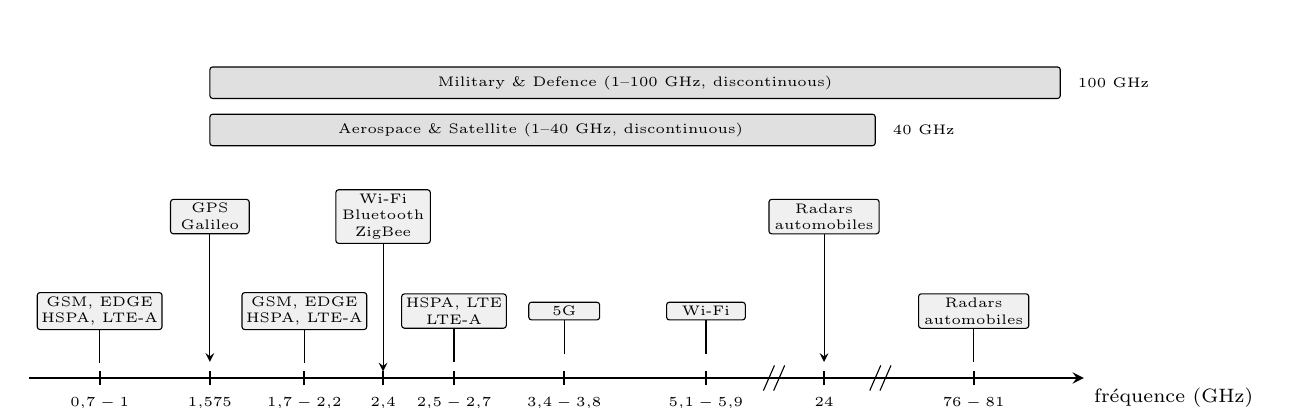
\begin{tikzpicture}[font=\tiny,>=stealth,
      band/.style={draw,fill=black!6,align=center,inner sep=1.5pt,rounded corners=1pt},
      ovl/.style={draw,fill=black!12,align=center,inner sep=1.5pt,rounded corners=1pt}]
    % axis
    \draw[->,thick] (0,0) -- (13.4,0) node[below right,font=\scriptsize] {fréquence (GHz)};
    \foreach \x in {0.9,2.3,3.5,4.5,5.4,6.8,8.6,10.1,12.0}
      \draw[thick] (\x,-0.09) -- (\x,0.09);
    % spectrum breaks
    \foreach \x in {9.4,10.75}
      {\draw (\x-0.07,-0.16) -- (\x+0.07,0.16); \draw (\x+0.06,-0.16) -- (\x+0.2,0.16);}
    % tick labels
    \node[below] at (0.9,-0.12) {$0{,}7-1$};
    \node[below] at (2.3,-0.12) {$1{,}575$};
    \node[below] at (3.5,-0.12) {$1{,}7-2{,}2$};
    \node[below] at (4.5,-0.12) {$2{,}4$};
    \node[below] at (5.4,-0.12) {$2{,}5-2{,}7$};
    \node[below] at (6.8,-0.12) {$3{,}4-3{,}8$};
    \node[below] at (8.6,-0.12) {$5{,}1-5{,}9$};
    \node[below] at (10.1,-0.12) {$24$};
    \node[below] at (12.0,-0.12) {$76-81$};
    % first row of service boxes
    \node[band,minimum width=1.2cm] (a) at (0.9,0.85) {GSM, EDGE\\HSPA, LTE-A};
    \node[band,minimum width=1.2cm] (b) at (3.5,0.85) {GSM, EDGE\\HSPA, LTE-A};
    \node[band,minimum width=1.0cm] (c) at (5.4,0.85) {HSPA, LTE\\LTE-A};
    \node[band,minimum width=0.9cm] (d) at (6.8,0.85) {5G};
    \node[band,minimum width=1.0cm] (e) at (8.6,0.85) {Wi-Fi};
    \node[band,minimum width=1.4cm] (f) at (12.0,0.85) {Radars\\automobiles};
    \foreach \n in {a,b,c,d,e,f} \draw (\n.south) -- ($(\n.south)+(0,-0.42)$);
    % second row
    \node[band,minimum width=1.0cm] (g) at (2.3,2.05) {GPS\\Galileo};
    \node[band,minimum width=1.2cm] (h) at (4.5,2.05) {Wi-Fi\\Bluetooth\\ZigBee};
    \node[band,minimum width=1.4cm] (i) at (10.1,2.05) {Radars\\automobiles};
    \foreach \n in {g,h,i} \draw[->] (\n.south) -- ($(\n.south)+(0,-1.62)$);
    % overlay service bars
    \draw[ovl] (2.3,2.95) rectangle (10.75,3.35);
    \node at (6.5,3.15) {Aerospace \& Satellite (1--40 GHz, discontinuous)};
    \node[right,font=\tiny] at (10.85,3.15) {40 GHz};
    \draw[ovl] (2.3,3.55) rectangle (13.1,3.95);
    \node at (7.7,3.75) {Military \& Defence (1--100 GHz, discontinuous)};
    \node[right,font=\tiny] at (13.2,3.75) {100 GHz};
  \end{tikzpicture}
  \caption*{\small Spectre radiofréquence (RF) \& applications. The most common
  consumer services all sit below $6$ GHz; satellite ($1$--$40$ GHz) and defence
  ($1$--$100$ GHz) overlay much of the spectrum, including part of the sub-$6$ GHz
  range, and use it discontinuously.}
\end{figure}

Les fréquences allouées aux applications les plus couramment utilisées
(téléphonie mobile, Wi-Fi, GPS, Bluetooth) sont situées à des fréquences
inférieures à $6$ GHz. Les satellites opèrent globalement entre $1$ GHz et
$40$ GHz mais avec une utilisation du spectre de manière \textit{discontinue} :
un satellite A utilise la bande de fréquences entre $1$\,--\,$2$ GHz, un
satellite B entre $4$\,--\,$6$ GHz, un satellite C entre $8$\,--\,$12$ GHz… et
certaines bandes de fréquences ne sont pas utilisées. Quant aux applications
militaires \& défense, elles sont présentes entre $1$\,--\,$100$ GHz de manière
également discontinue.

\begin{conclusion}
  La quasi-totalité des fréquences du spectre RF sont dédiées à une ou
  plusieurs applications : le spectre RF est \textit{saturé}. Spectrum is a
  scarce resource, which is why band allocations are fought over and why
  services are retired to free them. The GSM and EDGE allocations at
  $0{,}7$\,--\,$1$ GHz and $1{,}7$\,--\,$2{,}2$ GHz are scheduled for shutdown by
  the end of $2028$.
\end{conclusion}

\begin{remark}
  The upper automotive-radar band is quoted either as $76$\,--\,$79$ GHz or as
  $76$\,--\,$81$ GHz; the figure above uses the wider range. Either way the band
  sits in the millimetre-wave region just below $100$ GHz.
\end{remark}

\paragraph{3. Ils contiennent des circuits émetteurs et récepteurs}
Les systèmes de télécommunications contiennent des circuits électroniques
\textbf{émetteurs} (\textit{transmitters}, Tx) et \textbf{récepteurs}
(\textit{receivers}, Rx). Si les antennes constituent la partie visible de ces
émetteurs/récepteurs (même si les antennes sont de plus en plus cachées), elles
rayonnent et captent des signaux RF qui sont générés, modulés/démodulés,
mélangés, amplifiés, filtrés par des circuits électroniques qui eux, sont
toujours cachés.

\subsection{La propagation dans les systèmes de télécommunication numérique}
A modern system is digital at both ends and analogue in the middle. Supposons
que les bits de données $01101110\ldots$ --- voice, video, data --- doivent être
transmis au récepteur.

\begin{figure}[h!]
  \centering
  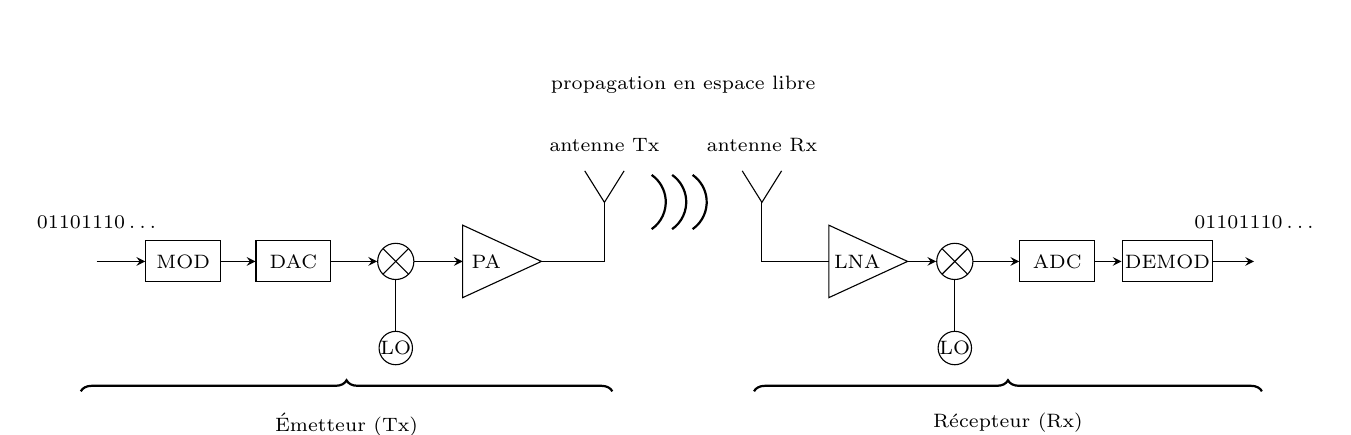
\begin{tikzpicture}[font=\scriptsize,>=stealth,
      blk/.style={draw,minimum width=0.95cm,minimum height=0.52cm,inner sep=1pt}]
    % --- transmitter ---
    \node[blk] (mod) at (0.6,0) {MOD};
    \node[blk] (dac) at (2.0,0) {DAC};
    \node[draw,circle,minimum size=0.46cm,inner sep=0pt] (mx1) at (3.3,0) {};
    \draw (mx1) ++(-0.16,-0.16) -- ++(0.32,0.32); \draw (mx1) ++(-0.16,0.16) -- ++(0.32,-0.32);
    \draw (4.15,-0.46) -- (4.15,0.46) -- (5.15,0) -- cycle;
    \node at (4.45,0) {PA};
    \node[draw,circle,minimum size=0.42cm,inner sep=0pt] (lo1) at (3.3,-1.1) {LO};
    \draw (mx1) -- (lo1);
    \draw[->] (-0.5,0) -- (mod.west);
    \node[align=center] at (-0.5,0.5) {$01101110\ldots$};
    \draw[->] (mod) -- (dac); \draw[->] (dac) -- (mx1);
    \draw[->] (mx1) -- (4.15,0);
    % Tx antenna
    \draw (5.15,0) -- (5.95,0) -- (5.95,0.75);
    \draw (5.70,1.15) -- (5.95,0.75) -- (6.20,1.15);
    \node[align=center] at (5.95,1.48) {antenne Tx};
    % --- propagation ---
    \foreach \i in {0,1,2} \draw[thick] (6.55+0.26*\i,0.41) arc (-55:55:0.42);
    \node[align=center] at (6.95,2.25) {propagation en espace libre};
    % --- receiver ---
    \draw (7.95,0.75) -- (7.95,0) -- (8.80,0);
    \draw (7.70,1.15) -- (7.95,0.75) -- (8.20,1.15);
    \node[align=center] at (7.95,1.48) {antenne Rx};
    \draw (8.80,-0.46) -- (8.80,0.46) -- (9.80,0) -- cycle;
    \node at (9.16,0) {LNA};
    \node[draw,circle,minimum size=0.46cm,inner sep=0pt] (mx2) at (10.4,0) {};
    \draw (mx2) ++(-0.16,-0.16) -- ++(0.32,0.32); \draw (mx2) ++(-0.16,0.16) -- ++(0.32,-0.32);
    \node[draw,circle,minimum size=0.42cm,inner sep=0pt] (lo2) at (10.4,-1.1) {LO};
    \draw (mx2) -- (lo2);
    \node[blk] (adc) at (11.7,0) {ADC};
    \node[blk] (dem) at (13.1,0) {DEMOD};
    \draw[->] (9.80,0) -- (mx2); \draw[->] (mx2) -- (adc); \draw[->] (adc) -- (dem);
    \draw[->] (dem.east) -- (14.2,0);
    \node[align=center] at (14.2,0.5) {$01101110\ldots$};
    % brace labels
    \draw[decorate,decoration={brace,amplitude=4pt},thick] (-0.7,-1.65) -- (6.05,-1.65)
      node[midway,below=4pt] {Émetteur (Tx)};
    \draw[decorate,decoration={brace,amplitude=4pt},thick] (7.85,-1.65) -- (14.3,-1.65)
      node[midway,below=4pt] {Récepteur (Rx)};
  \end{tikzpicture}
  \caption*{\small Schéma fonctionnel simplifié d'une communication RF.
  Everything between the DAC and the ADC is analogue.}
\end{figure}

Au niveau de l'émetteur, les bits sont soumis à un traitement numérique appelé
\textbf{modulation} (MOD) suivi d'une \textbf{conversion numérique/analogique}
(\textit{digital-to-analogue conversion}, DAC). Celle-ci consiste en la
conversion des bits de données (numérique) en signal analogique
\textbf{basse fréquence} (\textit{low frequency}, BF). À la sortie
du DAC, un \textbf{mélangeur} (\textit{mixer}) permet la transposition de ce
signal analogique BF vers les fréquences RF. Le terme « mélangeur » provient du
fait que le signal basse fréquence sortant du DAC est « mélangé » à un signal
haute fréquence provenant d'un \textbf{oscillateur local} (\textit{local
oscillator}, LO) pour donner un signal RF en sortie du mélangeur. Un
\textbf{amplificateur de puissance} (\textit{power amplifier}, PA) augmente alors
la puissance de ce signal RF qui est ensuite rayonné par l'antenne d'émission
(Tx).\\

Après s'être propagé dans l'air (subissant un très fort affaiblissement), le
signal RF est capté par l'antenne de réception (Rx). Le signal RF étant très
faible, un \textbf{amplificateur faible bruit} (\textit{low-noise amplifier},
LNA) est alors utilisé pour élever le niveau du signal reçu, puis un mélangeur
transpose le signal RF vers les fréquences BF. Enfin, un \textbf{convertisseur
analogique/numérique} (\textit{analogue-to-digital converter}, ADC) transforme
le signal analogique BF sous forme numérique, puis celui-ci est démodulé
(DEMOD) et les bits de données $01101110\ldots$ sont récupérés.

\begin{conclusion}
  En pratique, ce schéma peut illustrer la communication entre un smartphone et
  sa station de base, entre une box internet et le module Wi-Fi d'un PC, entre
  un smartphone et une enceinte Bluetooth, entre un satellite GPS et le module
  GPS installé dans une voiture. Whatever the service, the chain is the same,
  and the quantity that actually propagates is a \textbf{signal sinusoïdal
  analogique}. This is why a module on propagation and antennes is stated
  entirely in terms of sinusoidal waves even though the traffic is digital.
\end{conclusion}

\begin{example}[Digital modulation schemes]
  The digital modulator maps bits onto the parameters of a sinusoid:
  \begin{subpart}
    \item \textbf{Modulation d'amplitude} (\textit{amplitude modulation}), e.g.\
      OOK (\textit{on-off keying}):
      a burst of carrier means $1$, no carrier means $0$. The frame
      $10100110$ appears as bursts separated by silences.
    \item \textbf{Modulation de fréquence} (\textit{frequency modulation}),
      e.g.\ FSK (\textit{frequency-shift
      keying}): each symbol selects one of several carrier frequencies; with
      four tones a symbol carries two bits, $00$, $01$, $10$, $11$. The frame
      $10110100$ splits into the symbols $10$, $11$, $01$, $00$; the tone
      assignment runs fastest-to-slowest as $11$, $10$, $01$, $00$, so the $11$
      burst is the densest and the $00$ burst the sparsest.
    \item \textbf{Modulation de phase} (\textit{phase modulation}), e.g.\ BPSK
      (\textit{binary phase-shift
      keying}): $1$ and $0$ are carried by two carrier phases $\pi$ apart. The
      frame $10011010$ appears as a continuous sinusoid with phase reversals at
      the symbol boundaries.
  \end{subpart}
\end{example}

\subsection{Quel est l'intérêt de faire fonctionner ces systèmes aux fréquences RF ?}
Les fréquences RF sont utilisées dans les systèmes de communications pour
3 raisons principales.

\paragraph{1. La taille des antennes varie en $1/f$}
La taille des antennes varie de manière inversement proportionnelle à la
fréquence. Les antennes sont donc plus petites aux fréquences RF et sont ainsi
plus facilement intégrables dans des boîtiers au milieu de différents circuits
électroniques. The progression from an antenne cornet large enough to fill a
laboratory bench at $0.1$ GHz down to the few-millimetre antenne hidden inside
a mobile phone at $100$ GHz is a direct consequence of $\lambda=c/f$.

\paragraph{2. Les conditions de propagation sont relativement favorables}
Les signaux RF se propagent convenablement en milieu urbain, ils sont capables
de traverser les murs des bâtiments, les vitres, les parois des véhicules, la
végétation, ils sont relativement insensibles aux conditions climatiques ---
wind, rain, snow.

\begin{remark}
  Il convient cependant de rester mesuré lorsque l'on parle de conditions de
  propagation favorables pour les signaux RF. En effet, les ondes
  électromagnétiques se propagent avec une atténuation d'autant plus forte que
  la fréquence est élevée… et les fréquences RF étant par définition des
  fréquences très élevées, elles subissent par conséquent une très forte
  atténuation… qui peut cependant être compensée par amplification des signaux
  et adaptation d'impédance --- the subject of the rest of this part. Note
  also, with feeling, that the window glass of Télécom Paris is the exception
  that does not let RF through.
\end{remark}

\paragraph{3. Les larges bandes spectrales sont disponibles}
La transmission de données haut débit nécessite l'utilisation d'une large
bande de fréquence. Un signal qui transporte de l'information est un
\textbf{signal modulé} (\textit{modulated signal}) et un tel signal occupe dans
le spectre RF une largeur de bande non nulle. De manière générale, plus un
signal occupe une bande de fréquence large, plus il favorise la transmission de
données haut débit.

\begin{figure}[h!]
  \centering
  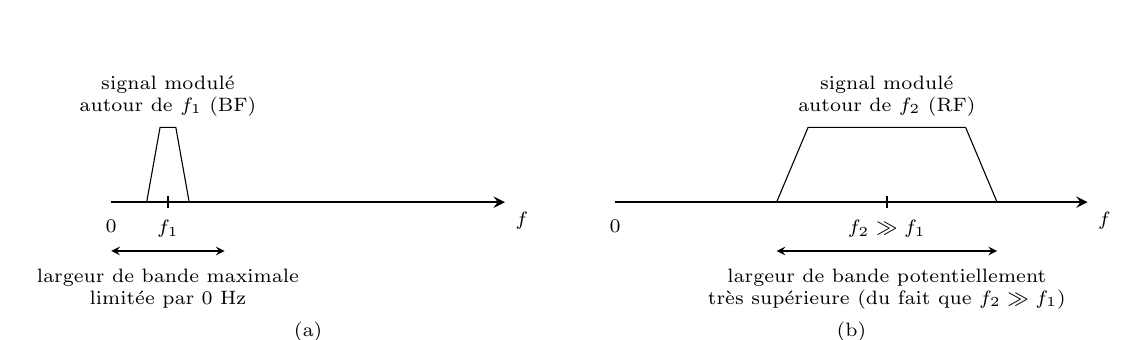
\begin{tikzpicture}[font=\scriptsize,>=stealth]
    % panel a
    \draw[->,thick] (0,0) -- (5.0,0) node[below right] {$f$};
    \draw (0.45,0) -- (0.62,0.95) -- (0.82,0.95) -- (0.99,0) -- cycle;
    \draw[thick] (0.72,-0.08) -- (0.72,0.08);
    \node[below] at (0.72,-0.1) {$f_1$};
    \node[below] at (0,-0.1) {$0$};
    \node[align=center] at (0.72,1.35) {signal modulé\\autour de $f_1$ (BF)};
    \draw[<->] (0,-0.62) -- (1.44,-0.62);
    \node[align=center,below] at (0.72,-0.72) {largeur de bande maximale\\limitée par $0$ Hz};
    \node at (2.5,-1.65) {(a)};
    % panel b
    \begin{scope}[xshift=6.4cm]
      \draw[->,thick] (0,0) -- (6.0,0) node[below right] {$f$};
      \draw (2.05,0) -- (2.45,0.95) -- (4.45,0.95) -- (4.85,0) -- cycle;
      \draw[thick] (3.45,-0.08) -- (3.45,0.08);
      \node[below] at (3.45,-0.1) {$f_2 \gg f_1$};
      \node[below] at (0,-0.1) {$0$};
      \node[align=center] at (3.45,1.35) {signal modulé\\autour de $f_2$ (RF)};
      \draw[<->] (2.05,-0.62) -- (4.85,-0.62);
      \node[align=center,below] at (3.45,-0.72) {largeur de bande potentiellement\\très supérieure (du fait que $f_2\gg f_1$)};
      \node at (3.0,-1.65) {(b)};
    \end{scope}
  \end{tikzpicture}
  \caption*{\small Signal modulé (a) autour d'une fréquence BF $f_1$ et (b)
  autour d'une fréquence RF $f_2 \gg f_1$. L'axe des abscisses représente la
  fréquence (en GHz) et l'axe des ordonnées représente la puissance du signal
  (en W).}
\end{figure}

Si on considère le cas d'un signal modulé centré sur une fréquence BF $f_1$ peu
élevée (quelques kHz ou MHz), la largeur de bande maximale de ce signal est
limitée par la fréquence $0$ Hz (car physiquement, les fréquences négatives
n'existent pas). Si on considère maintenant un signal modulé centré sur une
fréquence $f_2 \gg f_1$ située dans le spectre RF ($0.1$\,--\,$100$ GHz), sa
largeur de bande peut potentiellement être très supérieure du fait que cette
fréquence est très « éloignée » de la fréquence $0$ Hz. Only the RF-centred
signal supports high-rate data transmission.

\subsection{Spécificités de l'ingénierie RF}
Un signal RF de fréquence $1$ GHz n'est pas qu'un signal qui varie dans le
temps $10^{6}$ fois plus vite qu'un signal BF de fréquence $1$ kHz. Cela
implique aussi et surtout des effets remarquables. Les circuits RF possèdent des
spécificités qui leur sont propres et les différencient des circuits BF.

\subsubsection{L'approximation basses fréquences n'est plus valable}
L'ingénierie de l'électronique BF (montages à amplificateurs opérationnels,
amplificateur collecteur/émetteur commun, filtres actifs…) est basée sur
l'approximation qui n'est valable uniquement qu'aux fréquences BF, pour
lesquelles la longueur d'onde $\lambda=c/f$ est extrêmement grande --- that is,
large compared with the circuit. Aux fréquences RF, la longueur d'onde est petite.

\begin{figure}[h!]
  \centering
  \small
  \begin{tabular}{lccccccc}
    \toprule
    $f$       & $1$ kHz & $20$ kHz & $1$ GHz & $5$ GHz & $10$ GHz & $40$ GHz & $100$ GHz \\
    \midrule
    $\lambda$ & $30$ km & $15$ km  & $30$ cm & $6$ cm  & $3$ cm   & $7{,}5$ mm & $3$ mm \\
    \bottomrule
  \end{tabular}
  \caption*{\small $\lambda=c/f$ across the BF and RF ranges. BF circuits have
  $\lambda \approx$ km; RF circuits have $\lambda \approx$ mm to m.}
\end{figure}

Par conséquent, la taille des composants électroniques (transistors,
résistances, capacités, inductances), la longueur des pistes sur les circuits
imprimés (et circuits intégrés), et la longueur des câbles deviennent alors non
négligeables par rapport à $\lambda$ et/ou supérieures à $\lambda$.

\begin{conclusion}
  La \textbf{théorie dite des lignes de transmission} s'applique alors aux
  pistes, aux câbles et plus généralement aux circuits RF. This is the subject
  of the third part of the module.
\end{conclusion}

\begin{example}[Circuit dimensions are fractions of a wavelength]
  A $20$ Hz\,--\,$20$ kHz audio amplifier has $\lambda = 15$ km at $20$ kHz:
  nothing on the board is comparable to $\lambda$, and analysis in éléments
  localisés works. By contrast, les antennes \& circuits RF ci-dessous
  comportent des éléments de longueurs égales à des fractions de longueur
  d'onde $\lambda$ :
  \begin{subpart}
    \item a $1{,}03$\,--\,$1{,}09$ GHz amplificateur de puissance with
      $\lambda/4$ stubs ($\lambda = 30$ cm à $1$ GHz);
    \item a $5$\,--\,$6$ GHz bandpass filter built from $\lambda/4$ resonators
      ($\lambda = 6$ cm à $5$ GHz);
    \item l'antenne réseau de $4\times 4$ patchs fonctionnant à $10$ GHz : la
      dimension des patchs, optimisée pour cette fréquence centrale, a une
      longueur égale à $\lambda/2$ ($\lambda = 3$ cm à $10$ GHz);
    \item a $40{,}5$\,--\,$43{,}5$ GHz mélangeur, $1{,}5$ mm $\times$ $2$ mm in
      total, again with $\lambda/4$ sections ($\lambda = 7{,}5$ mm à
      $40$ GHz).
  \end{subpart}
  Pour une fréquence de fonctionnement double, cette dimension serait réduite
  par 2 --- and so would every one of these dimensions. Cette propriété
  s'applique également aux circuits RF autres que les antennes.
\end{example}

\subsubsection{Conséquences sur l'analyse, la conception, la fabrication et les mesures}
\paragraph{Analyse théorique} Application de la théorie des lignes de
transmission, l'utilisation des \textbf{paramètres S}. A dipôle such as an
antenne is described by the single coefficient
$[S]_{\text{antenna}}=[S_{11}]$; a quadripôle such as an RF
transistor by
\[[S]_{\text{transistor}}=\begin{pmatrix} S_{11} & S_{12}\\ S_{21} & S_{22}\end{pmatrix}.\]

\paragraph{Conception et design} La conception et le design sont largement
basés sur les notions de facteur de réflexion $\Gamma$ et
d'\textbf{adaptation d'impédance} (\textit{impedance matching}). Des logiciels de simulation de plus en plus sophistiqués et
exigeants en termes de puissance de calcul (logiciels de simulation
électromagnétiques 3D, notamment) permettent de faciliter la conception et
l'optimisation des designs des circuits RF.

\begin{example}[Why matching is not optional]
  Drive a $2\times 2$ antenne patch with $1$ mW and $0{,}6$ mW comes straight
  back out of the input, reflected by the \textbf{désadaptation d'impédance}
  (\textit{impedance mismatch}) --- only $0{,}4$ mW reaches the antenne. Drive
  an RF transistor with $1$ mW and $0{,}8$ mW is reflected: « $0.8$ mW !!! », a
  loss worth every exclamation mark. Each interface of an RF assembly is a place
  where power can be reflected away, so an antenne réseau de patchs is adapté
  at every one of its feed points.
\end{example}

\paragraph{Fabrication} La fabrication des antennes \& circuits RF nécessite
l'emploi de \textbf{graveuses} (\textit{PCB plotters}) mécaniques ou laser de
grande précision qui ne sont pas forcément nécessaires pour les circuits BF.

\paragraph{Instrumentation} Dans le domaine de l'instrumentation RF, la
principale grandeur physique mesurée est la \textbf{puissance} (en
instrumentation BF, c'est plutôt la tension et le courant) ou le rapport entre
2 valeurs de puissances. This difference is a habit of mind worth acquiring
early.

\begin{notation}
  Les mesures RF sont réalisées à l'aide d'un \textbf{analyseur de spectre}
  (\textit{spectrum analyser}) ou d'un \textbf{wattmètre} (\textit{power
  meter}) mais rarement à l'aide d'un oscilloscope (même si c'est possible) et
  \textit{jamais} d'un voltmètre/ampèremètre.
  L'\textbf{analyseur de réseaux vectoriel} (\textit{vector network analyser},
  VNA) permet de mesurer les paramètres S des circuits ou composants RF (ça
  inclut la caractérisation d'antennes). Le VNA est sans doute l'appareil de
  mesure le plus emblématique de l'instrumentation RF. Contrairement à tout
  autre équipement de mesure, le VNA a la particularité de nécessiter une
  procédure d'\textbf{étalonnage} (\textit{calibration}) avant chaque
  utilisation (car sans étalonnage du VNA, les mesures sont tout simplement
  fausses).
\end{notation}

\subsection{Problématiques de l'ingénierie RF : affaiblissement des signaux RF}

\begin{definition}[Le problème fondamental de l'ingénierie RF]
  La perte de puissance des signaux RF utiles (affaiblissement dû à la
  propagation dans les circuits ou sans fil, pertes par réflexion dues à une
  désadaptation d'impédance) est \textit{le} problème fondamental de
  l'ingénierie RF et les solutions techniques apportées en réponse sont
  l'\textbf{amplification} et l'\textbf{adaptation d'impédance}.
\end{definition}

Minimising attenuation is not an aesthetic concern: it bounds power
consumption and battery life at one end, and system functionality at the other.
Adaptation d'impédance optimises the power transfer and thereby guarantees that
the system works at all.

\subsubsection{Pertes dans les matériaux}
Dans les systèmes de télécommunications, les signaux se propagent
principalement dans l'air (dit « espace libre »), à travers des murs, des
vitres, de la végétation… mais également dans les circuits RF et les câbles.
L'atténuation dans les circuits RF et câbles est due à l'imperfection des
matériaux \textbf{conducteurs} (\textit{conductors}) et \textbf{diélectriques}
(\textit{dielectrics}) qui les constituent. The RF industry works
with metals (Cu, Al, Au), insulators (air, Teflon, alumina, quartz, fibreglass)
and semiconductors (Si, GaAs, GaN, SiC).

\begin{definition}[Origine des pertes]
  Dans les matériaux \textbf{conducteurs}, c'est la conductivité $\sigma$ non
  infinie (ou la résistivité $\rho = 1/\sigma$ non nulle) qui est responsable
  de l'atténuation (pertes) par \textbf{effet Joule} (\textit{Joule loss}) et
  effet de peau (ce dernier augmentant avec la fréquence). Dans les matériaux
  \textbf{diélectriques}, ce sont les propriétés de la permittivité électrique
  $\varepsilon$ qui expliquent l'atténuation des signaux RF.
\end{definition}

\subsubsection{Pertes dans les câbles}
The reference example is a typical commercial $1$ m câble coaxial. Le câble
montré dans cet exemple est issu d'un fabricant (Mini-Circuits) qui est un des
leaders du marché des composants RF. Les performances en termes d'atténuation
peuvent varier quelque peu d'un fabricant à l'autre mais restent du même ordre
de grandeur. The source drives $1$ mW $=0$ dBm into the cable and a wattmètre
reads what comes out.

\begin{figure}[h!]
  \centering
  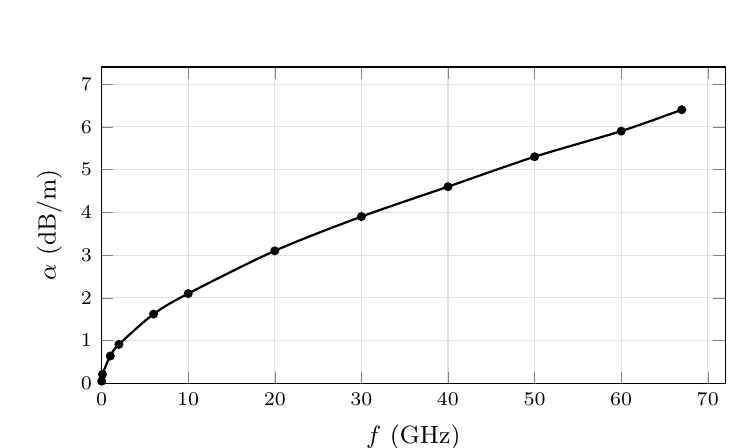
\begin{tikzpicture}
    \begin{axis}[width=9.5cm,height=5.6cm,
        xlabel={$f$ (GHz)},ylabel={$\alpha$ (dB/m)},
        xmin=0,xmax=72,ymin=0,ymax=7.4,
        xtick={0,10,20,30,40,50,60,70},ytick={0,1,2,3,4,5,6,7},
        grid=both,grid style={black!12},
        tick label style={font=\scriptsize},label style={font=\small}]
      \addplot[thick,mark=*,mark size=1.2pt,smooth] coordinates {
        (0.01,0.05) (0.1,0.21) (1,0.64) (2,0.91) (6,1.62) (10,2.1)
        (20,3.1) (30,3.9) (40,4.6) (50,5.3) (60,5.9) (67,6.4)};
    \end{axis}
  \end{tikzpicture}
  \caption*{\small Atténuation $\alpha$ des signaux RF dans un câble coaxial de
  longueur $1$ m, en fonction de la fréquence. $\alpha$ increases monotonically
  with frequency $\omega$.}
\end{figure}

\begin{figure}[h!]
  \centering
  \small
  \begin{tabular}{lccccccccc}
    \toprule
    $f$ & $10$ MHz & $0{,}1$ GHz & $1$ GHz & $2$ GHz & $6$ GHz & $10$ GHz & $20$ GHz & $40$ GHz & $67$ GHz \\
    \midrule
    $\alpha$ (dB/m) & $0{,}05$ & $0{,}21$ & $0{,}64$ & $0{,}91$ & $1{,}62$ & $2{,}1$ & $3{,}1$ & $4{,}6$ & $6{,}4$ \\
    $P_{\text{out}}$ (mW) & $0{,}99$ & $0{,}95$ & $0{,}86$ & $0{,}81$ & $0{,}69$ & $0{,}62$ & $0{,}49$ & $0{,}35$ & $0{,}23$ \\
    \bottomrule
  \end{tabular}
  \caption*{\small Output power of a $1$ m câble coaxial fed with
  $1$ mW $=0$ dBm.}
\end{figure}

\begin{example}[Reading the cable table]
  À $10$ MHz, $\alpha = 0{,}05$ dB/m, équivalent à $1\%$ d'atténuation de la
  puissance du signal, ce qui est négligeable. Par contre, à
  $1$ GHz (GSM à $890$\,--\,$960$ MHz), $\alpha = 0{,}64$ dB/m, soit environ
  $15\%$ d'atténuation, ce qui est loin d'être négligeable. À $6$ GHz (Wi-Fi à
  $5{,}2$\,--\,$5{,}7$ GHz), $\alpha = 1{,}62$ dB/m, soit environ $30\%$
  d'atténuation. Au-delà de $20$ GHz, $\alpha > 3$ dB/m, soit plus de $50\%$
  d'atténuation, et à $67$ GHz, $\alpha = 6{,}4$ dB/m, soit une puissance de
  signal atténuée de plus de $75\%$. Dans ce dernier cas, un signal ayant une
  puissance de $1$ mW à l'entrée du câble de $1$ m en ressort avec une
  puissance de $0{,}23$ mW.
\end{example}

\begin{conclusion}
  Attenuation of a signal RF is a serious issue in câble coaxial. For a
  signal BF it is not a concern at all. One metre of cable is a
  component, not a wire.
\end{conclusion}

\subsubsection{Affaiblissement en espace libre}
Si l'atténuation des signaux RF dans un câble peut être élevée, elle est
cependant bien inférieure à l'atténuation dans l'air.

\begin{definition}[Affaiblissement en espace libre]
  L'\textbf{affaiblissement en espace libre} (\textit{free-space path loss},
  FSPL) est la grandeur utilisée pour quantifier l'affaiblissement d'un signal
  RF dans l'air en fonction de la fréquence $f$ pour un signal se propageant
  entre une antenne d'émission (Tx) et une antenne de réception (Rx) séparées
  par une distance $d$ :
  \[\text{FSPL}=\left(\frac{4\pi d f}{c}\right)^{2},\qquad c=3\times 10^{8}\ \text{m/s}.\]
\end{definition}

The expression is stated here and used as a fact; its origin and derivation
come later with the bilan de liaison and the équation de Friis.
L'affaiblissement en espace libre FSPL augmente de manière
\textit{quadratique} en fonction de la fréquence $f$ et de la distance $d$
entre émetteur/récepteur. On exprime généralement cet affaiblissement en
échelle logarithmique :
\[\text{FSPL(dB)}=10\log_{10}\!\left(\frac{4\pi d f}{c}\right)^{2}
  =20\log_{10}(d)+20\log_{10}(f)-147{,}5,\]
with $d$ in metres and $f$ in hertz.

\begin{remark}
  The constant $-147{,}5$ is $20\log_{10}(4\pi/c)$ with $c$ in m/s; it is tied
  to those units. Feeding $d$ in km or $f$ in GHz changes the constant, so keep
  metres and hertz unless a formula explicitly says otherwise.
\end{remark}

\begin{figure}[h!]
  \centering
  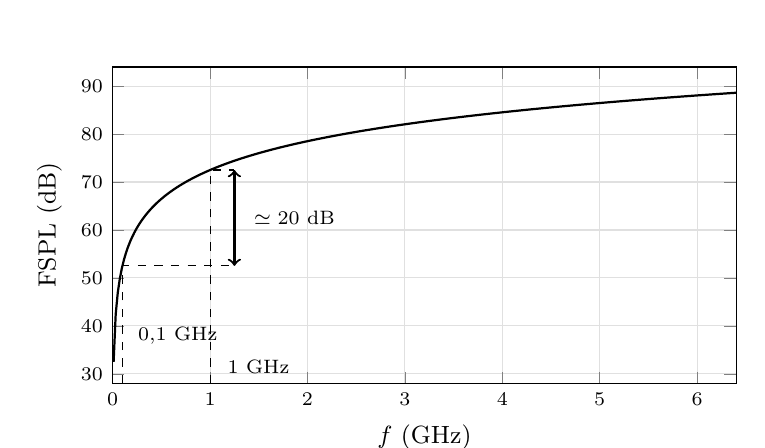
\begin{tikzpicture}
    \begin{axis}[width=9.5cm,height=5.6cm,
        xlabel={$f$ (GHz)},ylabel={FSPL (dB)},
        xmin=0,xmax=6.4,ymin=28,ymax=94,
        xtick={0,1,2,3,4,5,6},ytick={30,40,50,60,70,80,90},
        grid=both,grid style={black!12},
        tick label style={font=\scriptsize},label style={font=\small}]
      \addplot[thick,domain=0.01:6.4,samples=300]{72.5+20*log10(x)};
      \draw[dashed] (axis cs:0.1,28) -- (axis cs:0.1,52.5) -- (axis cs:1.25,52.5);
      \draw[dashed] (axis cs:1,28) -- (axis cs:1,72.5) -- (axis cs:1.25,72.5);
      \draw[<->,thick] (axis cs:1.25,52.5) -- (axis cs:1.25,72.5);
      \node[right,font=\scriptsize] at (axis cs:1.35,62.5) {$\simeq 20$ dB};
      \node[right,font=\scriptsize] at (axis cs:0.16,38) {$0{,}1$ GHz};
      \node[right,font=\scriptsize] at (axis cs:1.08,31.5) {$1$ GHz};
    \end{axis}
  \end{tikzpicture}
  \caption*{\small Atténuation en espace libre (FSPL) des signaux RF pour une
  distance émetteur/récepteur $d=100$ m.}
\end{figure}

\begin{example}[The $20$ dB that matters]
  Take $d = 100$ m. À $100$ MHz, le FSPL $=52{,}5$ dB tandis qu'à $1$ GHz (GSM à
  $890$\,--\,$960$ MHz), FSPL $=72{,}5$ dB, soit $20$ dB d'écart, ce qui
  signifie qu'un signal RF à la fréquence de $1$ GHz est $100$ fois plus
  atténué qu'un signal de $100$ MHz. Equivalently: a GSM $900$ MHz signal is
  attenuated $100$ times more than an FM radio signal at $88$\,--\,$108$ MHz
  over the same distance. L'affaiblissement des signaux devient beaucoup plus
  problématique aux fréquences RF qu'aux fréquences BF.
\end{example}

\begin{conclusion}
  Du fait de la très forte atténuation des signaux RF dans l'air, il est
  indispensable de les amplifier au niveau de l'émetteur d'une part
  (amplification de puissance, avant l'antenne Tx), et au niveau du récepteur
  d'autre part (amplification faible bruit, après l'antenne Rx).
  That is exactly why the PA and the LNA sit where they do in the functional
  diagram above, and why dispositifs d'adaptation d'impédance sit at every
  interface between them.
\end{conclusion}

\begin{remark}
  Tous les systèmes de télécommunications modernes possèdent des circuits
  électroniques qui remplissent les fonctions indiquées sur le schéma
  fonctionnel ci-dessus (modulation/démodulation numérique, conversion
  analogique/numérique \& numérique/analogique, mélange, oscillation,
  amplification de puissance/faible bruit, filtrage, rayonnement). Ces
  circuits sont complexes et la compréhension de leur fonctionnement
  nécessite des connaissances dans différents domaines (traitement du signal
  \& communications numériques, électronique numérique et analogique,
  électronique RF, antennes \& propagation RF). Celles-ci sont en pratique
  étudiées dans différentes UEs de 1ère année (ECE\_3TC21\_TP, APM\_3TC15\_TP,
  ECE\_3TC22\_TP) et surtout de 2ème année (filière TELECOM). This module owns
  the last two: RF electronics at the level of lignes de transmission and
  adaptation d'impédance, and antennes and propagation.
\end{remark}

\section{Propagation d'une onde électromagnétique}
Une onde électromagnétique (OEM) est une onde qui peut se propager dans le vide
ou un milieu et qui résulte des oscillations couplées d'un champ électrique
$\v{E}$ et magnétique $\v{H}$. For a wireless link, l'information est portée par
la \emph{puissance} de l'onde électromagnétique, so everything downstream ---
lignes de transmission, adaptation d'impédance, antennes, the bilan de liaison
--- rests on knowing how $\v{E}$ and $\v{H}$ travel and how much power they
transport.

This part restricts itself to the medium in which radio and hyperfréquence links
actually live: a diélectrique parfait that is linéaire, homogène and isotrope.
Dans ce cours, on s'intéresse principalement à la propagation des ondes radio et
hyperfréquences ($\lambda > 1$ mm) pour les télécommunications. Rappel : la
fréquence $f = 1$ GHz correspond à une longueur d'onde $\lambda = 30$ cm dans
l'air.

\begin{remark}
  Si ce chapitre permet de rappeler (ou de faire découvrir pour certains) les
  fondamentaux de la propagation d'une onde électromagnétique en milieu linéaire
  homogène et isotrope, il n'est \emph{pas} au programme du contrôle. It is
  nonetheless the vocabulary --- $\eta$, $k_z$, $v_\varphi$, the vecteur de
  Poynting --- that every later chapter reuses without redefining.
\end{remark}

\begin{notation}
  In the French convention the vector operators are written
  $\overrightarrow{\mathrm{rot}}$, $\mathrm{div}$,
  $\overrightarrow{\mathrm{grad}}$; these notes write $\curl$, $\div$ and
  $\grad$ for the same three. The cross product is written $\wedge$
  throughout. Vectors are bold: $\v{E}$, $\v{H}$, $\v{k}$.\\

  Two symbols collide and must not be confused: $j$ is the imaginary unit,
  while $\v{j}(\v{r},t)$ is the current-density vector.\\

  The complex convention of the course is $e^{+j\omega t}$ for the time factor,
  so a wave travelling towards increasing $z$ carries
  $e^{j(\omega t - k_z z)}$ --- the phase spatiale enters with a \emph{minus}
  sign. Every result below inherits that sign choice.
\end{notation}

\subsection{L'onde électromagnétique dans un milieu linéaire homogène isotrope}

\begin{definition}[Milieu linéaire homogène isotrope (\textit{linear homogeneous isotropic medium}, MLHI)]
  Un milieu matériel est
  \begin{itemize}
    \item \textbf{homogène} (\textit{homogeneous}) s'il a la particularité
      d'avoir des propriétés physiques (permittivité, perméabilité,
      conductivité…) identiques en tout point de l'espace ;
    \item \textbf{isotrope} (\textit{isotropic}) s'il a la particularité
      d'avoir des propriétés physiques (permittivité, perméabilité,
      conductivité…) identiques dans toutes les directions ;
    \item \textbf{linéaire} (\textit{linear}) si la permittivité et la
      perméabilité, le caractérisant, sont indépendantes de l'amplitude du
      champ électromagnétique appliqué.
  \end{itemize}
\end{definition}

Dans le domaine des télécommunications radiofréquence, ces types de milieu sont
majoritaires (ex. : vide, air, diélectrique…) --- which is why the whole course
is written for them.

\subsubsection{Généralités sur les milieux diélectriques}

Un \textbf{milieu diélectrique} est un milieu isolant --- qui ne contient pas
des charges libres et mobiles. Les électrons présents dans un milieu
diélectrique ne peuvent pas, par définition, se déplacer sur des grandes
distances --- comme c'est le cas dans les conducteurs --- mais ont la
possibilité d'avoir des mouvements d'amplitude très petite sous l'action d'un
champ électrique $\v{E}$. Ces mouvements sont des mouvements d'oscillation
autour du noyau atomique. Le nuage électronique se déforme créant ainsi un
dipôle électrostatique (a dipole moment $\v{P}$) and hence a polarisation of the
medium. Polarisation proper --- that of the wave --- is taken up again in the
chapter on antennes.

\subsubsection{Relations constitutives des milieux diélectriques}

On appelle \textbf{relations constitutives} (\textit{constitutive relations})
d'un milieu diélectrique l'ensemble des effets du milieu sur une onde
électromagnétique. Les principales relations décrivent la susceptibilité
électrique, la permittivité diélectrique, la perméabilité magnétique et la
conductivité.

\paragraph{Susceptibilité électrique et permittivité diélectrique.}
La \textbf{susceptibilité électrique} (\textit{electric susceptibility}) $\chi$
est une grandeur caractérisant la polarisation $\v{P}$ créée par un champ
électrique $\v{E}$. L'amplitude du champ électrique utilisé est suffisamment
faible pour que la polarisation vérifie la relation suivante :
\[
  \v{P} = \varepsilon_0\,\chi\,\v{E},
  \qquad \varepsilon_0 = 8.854\,187\times 10^{-12}\ \text{F}\cdot\text{m}^{-1},
\]
où $\varepsilon_0$ est la constante diélectrique du vide. La susceptibilité
électrique $\chi$ est un nombre complexe sans dimension (le milieu, dans ce cas,
est qualifié de linéaire). Elle permet d'exprimer la permittivité diélectrique
relative par la relation :
\[
  \varepsilon_r = 1 + \Re(\chi).
\]

L'influence qu'un champ électrique $\v{E}$ a sur l'organisation des charges
électriques dans un matériau donné est définie par l'\textbf{induction
électrique} (\textit{electric displacement}) $\v{D}$. La relation entre ces
grandeurs, dans le cas d'un MLHI, est :
\[
  \v{D} = \varepsilon\,\v{E},
  \qquad\text{with}\qquad
  \varepsilon_r = \frac{\varepsilon}{\varepsilon_0},
\]
où $\varepsilon$ désigne la \textbf{permittivité} (\textit{permittivity}) sous
forme scalaire. Le vide est choisi comme milieu de référence, car il est
linéaire, homogène, isotrope avec réponse instantanée.

\begin{definition}[Angle de perte (\textit{loss angle})]
  Dans un milieu diélectrique réel, la conductivité $\sigma$ est faible mais pas
  nulle. On parle alors de \textbf{pertes diélectriques} (\textit{dielectric
  losses}). Ces pertes se traduisent en définissant une permittivité complexe
  dépendante de la fréquence ou de la pulsation de l'onde électromagnétique se
  propageant dans le milieu :
  \[
    \varepsilon(\omega) = \varepsilon'(\omega) - j\,\varepsilon''(\omega),
  \]
  et ces pertes sont souvent très faibles : la partie imaginaire est donc très
  petite devant la partie réelle, $\varepsilon''(\omega) \ll
  \varepsilon'(\omega)$. On définit alors un angle de perte $\delta$ par la
  relation :
  \[
    \tan(\delta) = \frac{\varepsilon''(\omega)}{\varepsilon'(\omega)}.
  \]
\end{definition}

Cette appellation s'explique par le fait que cet angle $\delta$ est l'angle
formé par la direction des vecteurs champ électrique $\v{E}$ et induction
électrique $\v{D}$, which are no longer collinear once $\varepsilon$ is complex.
Note the minus sign in the definition of $\varepsilon(\omega)$ --- it is what
makes a passif lossy medium sit in the fourth quadrant under the
$e^{+j\omega t}$ convention. En télécommunications, pour optimiser une liaison,
on essaiera de minimiser ces pertes.

\begin{figure}[h!]
  \centering
  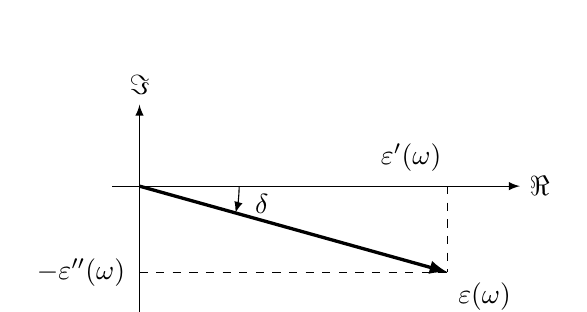
\begin{tikzpicture}[>=latex,scale=1.15]
    \draw[->] (-0.3,0) -- (4.2,0) node[right]{$\Re$};
    \draw[->] (0,-1.5) -- (0,0.9) node[above]{$\Im$};
    \draw[->,very thick] (0,0) -- (3.4,-0.95)
      node[below right]{$\varepsilon(\omega)$};
    \draw[dashed] (3.4,0) -- (3.4,-0.95);
    \draw[dashed] (0,-0.95) -- (3.4,-0.95);
    \node[above] at (3.0,0.05) {$\varepsilon'(\omega)$};
    \node[left] at (-0.05,-0.95) {$-\varepsilon''(\omega)$};
    \draw[->] (1.1,0) arc (0:-15.6:1.1);
    \node at (1.35,-0.2) {$\delta$};
  \end{tikzpicture}
  \caption*{\small The complex permittivité of a lossy diélectrique and the angle
  de perte $\delta$, with $\tan\delta = \varepsilon''/\varepsilon'$. For a
  diélectrique parfait $\varepsilon'' = 0$ and $\delta = 0$.}
\end{figure}

\begin{remark}
  En optique, on parlera plutôt d'\textbf{indice de réfraction}
  (\textit{refractive index}) du milieu, noté $n$, que de permittivité. La
  relation ci-dessous exprime le lien entre ces 2 notions :
  \[ n = \sqrt{\varepsilon_r}. \]
\end{remark}

\paragraph{Perméabilité magnétique.}
La \textbf{perméabilité magnétique} (\textit{permeability}) caractérise la
faculté d'un matériau à modifier un champ magnétique $\v{H}$, c'est-à-dire à
modifier les lignes de flux magnétique. Si le milieu a un comportement linéaire
et isotrope, le champ magnétique et l'\textbf{induction magnétique}
(\textit{magnetic induction}) $\v{B}$ sont reliés par la relation :
\[
  \v{B} = \mu\,\v{H},
  \qquad
  \mu = \mu_0\,\mu_r,
  \qquad
  \mu_0 = 4\pi\times 10^{-7}\ \text{H}\cdot\text{m}^{-1},
\]
où $\mu$ est la perméabilité magnétique du matériau (en henry par mètre, H/m)
et $\mu_r$ la perméabilité relative du matériau.

Dans l'air, le vide, les gaz, le cuivre, l'aluminium, la terre, etc.,
$\mu_r \approx 1$, ces matériaux ne pouvant alors canaliser le champ
magnétique. \textbf{Nous admettrons dans ce cours que, pour un milieu
diélectrique, $\mu_r = 1$ et que les pertes magnétiques des matériaux sont
négligeables.} Dans les milieux anisotropes, $\mu_r \ne 1$. Ces milieux
permettent la réalisation de fonctions spécifiques pour la propagation d'ondes
électromagnétiques. Nous présentons une introduction de ces milieux dans le
dernier chapitre.

\paragraph{Conductivité électrique.}
La \textbf{conductivité électrique} (\textit{conductivity}) caractérise
l'aptitude d'un matériau à laisser les charges électriques se déplacer
librement et donc permettre le passage d'un courant électrique. Elle est notée
$\sigma$ et s'exprime en $\text{S}\cdot\text{m}^{-1}$. La conductivité
s'exprime par la relation suivante, appelée aussi \textbf{loi d'Ohm locale}
(\textit{local Ohm's law}) :
\[
  \v{j} = \sigma\,\v{E},
\]
où $\v{j}$ représente la densité de courant exprimée en
$\text{A}\cdot\text{m}^{-2}$. Pour un milieu \textbf{diélectrique parfait}
(\textit{perfect dielectric}), la conductivité est nulle, $\sigma = 0$, and
therefore $\v{j} = \v{0}$.

\begin{conclusion}[Les trois relations constitutives d'un MLHI]
  \[
    \begin{array}{lll}
      \v{D} = \varepsilon\,\v{E} & \quad & \text{defines the permittivity} \\[2pt]
      \v{B} = \mu\,\v{H}         & \quad & \text{defines the permeability} \\[2pt]
      \v{j} = \sigma\,\v{E}      & \quad & \text{defines the conductivity}
    \end{array}
  \]
  with $\varepsilon = \varepsilon_0\varepsilon_r$, $\mu = \mu_0\mu_r$, and, for
  the diélectrique parfait used from here on, $\sigma = 0$ and $\mu_r = 1$.
\end{conclusion}

\subsection{Onde électromagnétique plane progressive monochromatique dans un MLHI diélectrique}

\subsubsection{Onde plane progressive}

\begin{definition}[Onde plane progressive (\textit{plane progressive wave})]
  Une onde électromagnétique est dite \textbf{plane} lorsque, pour une
  direction de propagation, les champs $\v{E}$ et $\v{H}$ conservent la même
  amplitude et même phase en tout point d'un plan orthogonal à la direction de
  propagation. La conséquence est que les variations du champ
  électromagnétique ne dépendent que de la direction de propagation. Une onde
  plane \textbf{progressive} indique que la propagation ne se fait que dans un
  sens, à partir de la source.
\end{definition}

Une onde plane est une \emph{approximation} dans le sens où c'est une
observation d'une onde dans un domaine limité de l'espace. Il suffit que les
\textbf{fronts d'onde} (\textit{wavefronts}) soient suffisamment plans et
parallèles dans le volume considéré ou en d'autres termes que l'on se trouve
suffisamment loin de la source émettant le champ électromagnétique pour pouvoir
justifier cette approximation. Dans le domaine des télécommunications radio, la
source est une antenne qui rayonne des ondes sphériques. Dans une direction
donnée et lorsqu'on est suffisamment loin, on peut considérer que localement
nous avons une onde plane.

\begin{definition}[Zones de champ rayonné par une antenne]
  Le rayonnement produit par une antenne de dimension $D$ n'est pas uniforme
  (it varies with distance). Il existe
  \begin{itemize}
    \item une \textbf{zone de champ proche} (\textit{near-field zone}),
      composée de la \textbf{zone de Rayleigh} (\textit{Rayleigh zone}) et de
      la \textbf{zone de Fresnel} (\textit{Fresnel zone}), où le front d'onde
      n'est pas plan ;
    \item la \textbf{zone de champ lointain} (\textit{far-field zone}) ou
      \textbf{zone de Fraunhofer} (\textit{Fraunhofer zone}), dont le début est
      situé à une distance
      \[ \frac{2D^2}{\lambda} \]
      de l'antenne, où $\lambda$ représente la longueur d'onde du signal émis.
  \end{itemize}
  C'est dans la zone de Fraunhofer que les ondes sont considérées localement
  planes.
\end{definition}

\begin{figure}[h!]
  \centering
  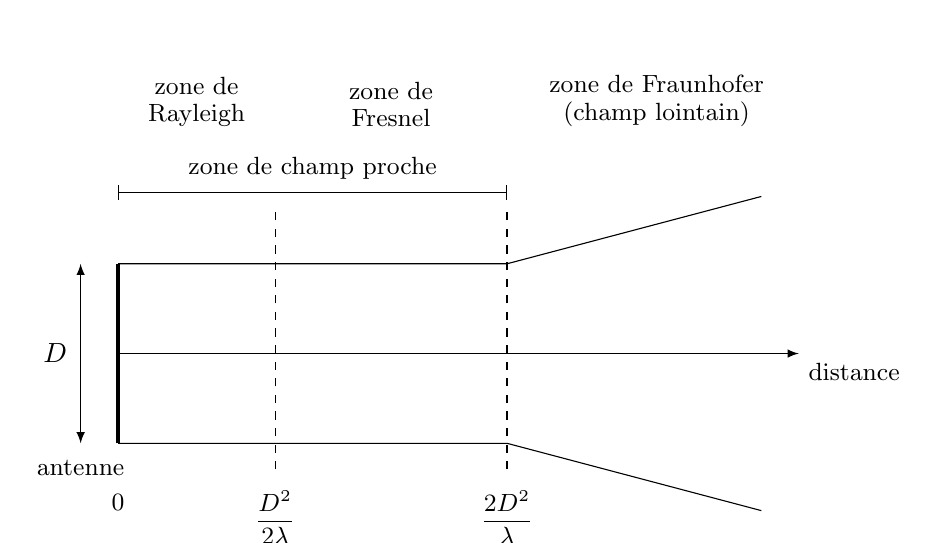
\begin{tikzpicture}[>=latex,scale=0.95]
    % aperture
    \draw[very thick] (0,-1.2) -- (0,1.2);
    \draw[<->] (-0.5,-1.2) -- (-0.5,1.2);
    \node[left] at (-0.55,0) {$D$};
    \node[below] at (-0.5,-1.3) {\small antenne};
    % beam
    \draw (0,1.2) -- (5.2,1.2) -- (8.6,2.1);
    \draw (0,-1.2) -- (5.2,-1.2) -- (8.6,-2.1);
    % zone boundaries
    \draw[dashed] (2.1,-1.55) -- (2.1,1.95);
    \draw[dashed] (5.2,-1.55) -- (5.2,1.95);
    % axis
    \draw[->] (0,0) -- (9.1,0) node[below right]{\small distance};
    % distance ticks, kept below the beam
    \node[below] at (0,-1.75) {\small $0$};
    \node[below] at (2.1,-1.7) {\small $\dfrac{D^2}{2\lambda}$};
    \node[below] at (5.2,-1.7) {\small $\dfrac{2D^2}{\lambda}$};
    % near-field bracket
    \draw[|-|] (0,2.15) -- (5.2,2.15);
    \node[above] at (2.6,2.2) {\small zone de champ proche};
    % zone labels
    \node[above,align=center] at (1.05,2.9) {\small zone de\\[-2pt]\small Rayleigh};
    \node[above,align=center] at (3.65,2.9) {\small zone de\\[-2pt]\small Fresnel};
    \node[above,align=center] at (7.2,2.9)
      {\small zone de Fraunhofer\\[-2pt]\small (champ lointain)};
  \end{tikzpicture}
  \caption*{\small Représentation des zones de champ rayonné par une antenne de
  dimension $D$. The plane-wave approximation --- and with it everything in
  this chapter --- is only legitimate beyond $2D^2/\lambda$.}
\end{figure}

Dans la zone de champ lointain, les champs $\v{E}(\v{r},t)$ et
$\v{H}(\v{r},t)$ sont perpendiculaires entre eux et perpendiculaires à la
direction de propagation. Ce type d'onde rencontrée dans les milieux
diélectriques MLHI est appelé onde \textbf{transverse électrique magnétique}
(\textit{transverse electromagnetic}, TEM).

\begin{remark}
  Il n'y aura donc \emph{pas de composante longitudinale} des champs $\v{E}$ et
  $\v{H}$ pour une onde TEM. Three vectors $\v{E}$, $\v{H}$, $\v{k}$ form a
  \textbf{trièdre direct} (\textit{right-handed trihedron}).
\end{remark}

\begin{figure}[h!]
  \centering
  \begin{tikzpicture}[>=latex,scale=1.1]
    \fill[black!7] (-1.5,-1.5) -- (0.55,-0.75) -- (0.55,1.65) -- (-1.5,0.9) -- cycle;
    \draw[black!45] (-1.5,-1.5) -- (0.55,-0.75) -- (0.55,1.65) -- (-1.5,0.9) -- cycle;
    \node[below] at (-0.5,-1.55) {\small plan d'onde};
    \draw[->,very thick] (0,0) -- (0,1.7) node[above]{$\v{E}$};
    \draw[->,very thick] (0,0) -- (-1.55,-0.58) node[left]{$\v{H}$};
    \draw[->,very thick] (0,0) -- (2.6,0)
      node[right,align=left]{$\v{k}$\\[-2pt]\small direction de propagation};
    \draw (0,0.28) -- (0.28,0.28) -- (0.28,0);
    \node[below left] at (0,0) {\small $O$};
  \end{tikzpicture}
  \caption*{\small Représentation d'une onde TEM : $\v{E} \perp \v{H} \perp
  \v{k}$, both fields lying in the wave plane, $\v{k}$ normal to it.}
\end{figure}

\subsubsection{Onde plane progressive monochromatique}

\begin{definition}[Onde monochromatique (\textit{monochromatic wave})]
  Une onde est \textbf{monochromatique} lorsque les champs $\v{E}$ et $\v{H}$,
  qui la décrivent, ne contiennent qu'une composante fréquentielle $f$ ou une
  seule pulsation $\omega = 2\pi f$. Ceci correspond donc à une onde dont la
  forme est sinusoïdale en fonction du temps et de l'espace.
\end{definition}

Dans un milieu MLHI où l'espace est matérialisé par le système de vecteur
unitaire $\v{u}(\v{u}_x,\v{u}_y,\v{u}_z)$ et $\v{r}(x,y,z)$ représentant un
point, les champs d'une \textbf{onde plane progressive monochromatique}
(\textit{plane progressive monochromatic wave}, OPPM) s'écrivent ainsi :
\[
  \begin{aligned}
    \v{E}(\v{r},t) &= \v{E}(\v{r})\cos\!\big(\omega t - \varphi(\v{r})\big) \\
    \v{H}(\v{r},t) &= \v{H}(\v{r})\cos\!\big(\omega t - \varphi(\v{r})\big)
  \end{aligned}
\]
Pour pouvoir étudier les phénomènes de propagation il est pratique de
représenter ces champs dans leur forme complexe :
\[
  \begin{aligned}
    \v{E}(\v{r},t) &= \v{E}(\v{r})\,e^{\,j(\omega t - \varphi(\v{r}))} \\
    \v{H}(\v{r},t) &= \v{H}(\v{r})\,e^{\,j(\omega t - \varphi(\v{r}))}.
  \end{aligned}
\]
Ici, $\v{E}(\v{r})$ et $\v{H}(\v{r})$ sont 2 vecteurs dont les composantes sont
transverses à la direction de propagation; which transverse directions they
pick out is the question of polarisation.\\

L'argument de l'exponentielle représente la phase des champs, and it splits in
two: le produit $\omega t$ représente la \textbf{phase temporelle}
(\textit{temporal phase}) et $\varphi(\v{r})$ la \textbf{phase spatiale}
(\textit{spatial phase}) de l'onde au vecteur position $\v{r}(x,y,z)$.

\paragraph{Variation spatiale / variation temporelle.}
Imaginons que l'on puisse arrêter le temps… On fige alors la propagation de
l'onde : on obtient la \textbf{longueur d'onde}, sur l'axe de propagation $OZ$,
en observant une période d'un signal sinusoïdal sur cet axe :
\[
  \boxed{\ \lambda = \frac{c}{f\sqrt{\varepsilon_r}}\ }
\]
où $c$ est la vitesse de la lumière dans le vide. Maintenant, imaginons un
observateur situé à l'abscisse $z$. Cet observateur va voir une variation
sinusoïdale d'amplitude de l'onde en fonction du temps. Cette variation
d'amplitude cyclique est faite sur une \textbf{période} déterminée par la
relation :
\[
  T = \frac{1}{f} = \frac{2\pi}{\omega}.
\]

\begin{figure}[h!]
  \centering
  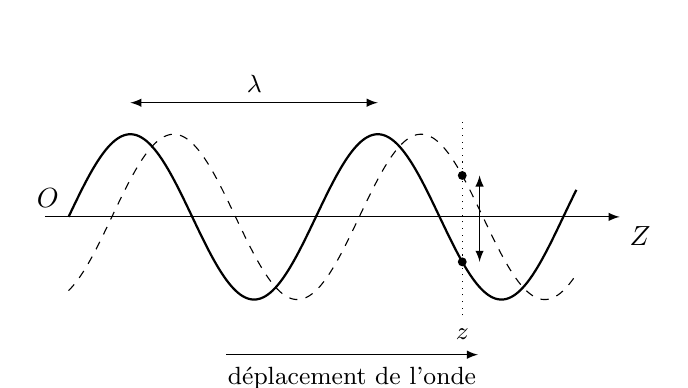
\begin{tikzpicture}[>=latex,scale=1.0]
    \draw[->] (-0.3,0) -- (7.0,0) node[below right]{$Z$};
    \node[above left] at (0,0) {$O$};
    \draw[thick,domain=0:12.9,samples=220,smooth,variable=\x]
      plot ({0.5*\x},{1.05*sin(deg(\x))});
    \draw[dashed,domain=0:12.9,samples=220,smooth,variable=\x]
      plot ({0.5*\x},{1.05*sin(deg(\x-1.1))});
    \draw[<->] (0.785,1.45) -- (3.927,1.45);
    \node[above] at (2.36,1.45) {\small $\lambda$};
    \draw[dotted] (5.0,-1.25) -- (5.0,1.25);
    \node[below] at (5.0,-1.3) {\small $z$};
    \fill (5.0,-0.571) circle (1.6pt);
    \fill (5.0,0.526) circle (1.6pt);
    \draw[<->] (5.22,-0.571) -- (5.22,0.526);
    \draw[->] (2.0,-1.75) -- (5.2,-1.75);
    \node[below] at (3.6,-1.78) {\small déplacement de l'onde};
  \end{tikzpicture}
  \caption*{\small En trait continu, l'évolution spatiale de l'onde à l'instant
  $t$ ; en pointillé, l'évolution spatiale de l'onde à l'instant
  $t + \Delta t$ avec $\Delta t < T$. The two dots are the amplitudes the
  observer at abscissa $z$ reads at the two instants: one period $\lambda$ in
  space, one period $T$ in time, the same wave.}
\end{figure}

\subsubsection{Vecteur d'onde $\v{k}$}

\begin{definition}[Vecteur d'onde (\textit{wave vector})]
  Le vecteur d'onde $\v{k}$ est un vecteur perpendiculaire au plan ou front
  d'onde et indique la direction de propagation. Sa norme correspond au
  \textbf{nombre d'onde} (\textit{wavenumber})
  \[
    \|\v{k}\| = k = \frac{2\pi}{\lambda}.
  \]
\end{definition}

De manière générale, le vecteur d'onde est défini par ses coordonnées
$\v{k}(k_x,k_y,k_z)$ exprimées dans un repère cartésien $(O,X,Y,Z)$. Dans ce
cas, on exprime la phase spatiale au point $\v{r}(x,y,z)$ :
\[
  \varphi(\v{r}) = \varphi_0 + \v{k}\cdot\v{r}
                 = \varphi_0 + \big(k_x x + k_y y + k_z z\big),
\]
où $\varphi_0$ représente la phase de l'onde à l'origine, choisie
arbitrairement car inconnue; the course sets $\varphi_0 = 0$.\\

Dans un milieu diélectrique parfait MLHI et pour une OPPM (TEM), on choisit
dans la suite du cours, par convention et simplification, une composante unique
de $\v{k}$ suivant l'axe $OZ$ :
\[
  \v{k}(0,0,k_z).
\]
Les champs $\v{E}$ et $\v{H}$ seront alors perpendiculaires entre eux et
perpendiculaires à $\v{k}$, le tout formant un trièdre direct.

\begin{conclusion}[OPPM dans un milieu MLHI se propageant selon $OZ$]
  \[
    \begin{aligned}
      \v{E}(z,t) &= \v{E}(z)\,e^{\,j(\omega t - k_z z)} \\
      \v{H}(z,t) &= \v{H}(z)\,e^{\,j(\omega t - k_z z)}
    \end{aligned}
  \]
\end{conclusion}

\subsection{Équations de Maxwell appliquées à une OPPM dans un milieu MLHI}

Les \textbf{équations de Maxwell} (\textit{Maxwell's equations}, 1864) sont des
lois fondamentales de la physique. Elles constituent la base de
l'électromagnétisme. Elles donnent ainsi un cadre mathématique précis au
concept fondamental de champ. On note $\rho$ la densité volumique de charge
électrique au point $\v{r}$ à l'instant $t$, et $\v{j}(\v{r},t)$ le vecteur
densité de courant --- attention à ne pas le confondre avec le $j$ issu des
nombres complexes.

\subsubsection{Définition des équations de Maxwell}

\begin{definition}[Maxwell--Faraday]
  L'équation de Maxwell--Faraday décrit comment la variation d'un champ
  magnétique peut induire un champ électrique. Ce courant induit est utilisé
  dans de nombreux générateurs électriques : un aimant en rotation crée un champ
  magnétique en mouvement qui génère un champ électrique dans un fil à
  proximité. Elle est définie ainsi :
  \[
    \curl \v{E} = -\frac{\del \v{B}}{\del t}
    \qquad\xrightarrow{\ \v{B} = \mu\v{H}\ }\qquad
    \curl \v{E} = -\mu\,\frac{\del \v{H}}{\del t}.
  \]
\end{definition}

\begin{definition}[Maxwell--Ampère]
  L'équation de Maxwell--Ampère énonce que les champs magnétiques peuvent être
  générés de deux manières : par les courants électriques (c'est le théorème
  d'Ampère) et par la variation d'un champ électrique (c'est l'apport de
  Maxwell sur cette loi) :
  \[
    \curl \v{H} = \v{j} + \frac{\del \v{D}}{\del t}
    \qquad\xrightarrow{\ \v{D} = \varepsilon\v{E}\ }\qquad
    \curl \v{H} = \v{j} + \varepsilon\,\frac{\del \v{E}}{\del t}.
  \]
  Dans le cas particulier d'un milieu diélectrique parfait MLHI de permittivité
  $\varepsilon$, la densité de courant est nulle, $\v{j} = \v{0}$, car il n'y a
  pas de charges électriques mobiles ou $\sigma = 0$, et on peut résumer cette
  équation par :
  \[
    \curl \v{H} = \varepsilon\,\frac{\del \v{E}}{\del t}.
  \]
\end{definition}

\begin{definition}[Maxwell--Gauss]
  Cette loi relie le flux électrique à travers n'importe quelle surface de Gauss
  fermée avec la charge électrique contenue dans le volume délimité par cette
  surface ; le champ électrique est orienté des charges positives vers les
  charges négatives :
  \[
    \div \v{D} = \rho
    \qquad\xrightarrow{\ \v{D} = \varepsilon\v{E}\ }\qquad
    \div \v{E} = \frac{\rho}{\varepsilon}.
  \]
  Dans le cas particulier d'un milieu diélectrique parfait MLHI, la densité
  volumique de charge électrique est nulle, $\rho = 0$ ; on peut alors
  simplifier l'équation par $\div \v{E} = 0$.
\end{definition}

\begin{definition}[Maxwell--Thomson]
  Le flux magnétique total à travers n'importe quelle surface de Gauss est nul :
  \[
    \div \v{B} = 0,
    \qquad\text{hence in a perfect MLHI dielectric}\qquad
    \div \v{H} = 0.
  \]
\end{definition}

\begin{remark}
  Les cas d'un diélectrique imparfait et d'un conducteur imparfait font
  apparaitre une densité de courant $\v{j}$ non nulle dans le milieu; the
  consequences for propagation --- attenuation, complex nombre d'onde --- are
  the subject of a later chapter.
\end{remark}

\begin{conclusion}[Équations de Maxwell généralisées et simplifiées]
  Les équations de Maxwell généralisées sont :
  \[
    \left\{
      \begin{aligned}
        \curl \v{E} &= -\mu\,\frac{\del \v{H}}{\del t} \\
        \curl \v{H} &= \v{j} + \varepsilon\,\frac{\del \v{E}}{\del t} \\
        \div \v{D}  &= \rho \\
        \div \v{B}  &= 0
      \end{aligned}
    \right.
  \]
  Pour une OPPM se propageant dans un milieu MLHI diélectrique parfait, de
  permittivité $\varepsilon = \varepsilon_0\varepsilon_r$ et de perméabilité
  $\mu_0$ ($\mu_r = 1$), les équations de Maxwell se simplifient ainsi :
  \[
    \left\{
      \begin{aligned}
        \curl \v{E} &= -\mu_0\,\frac{\del \v{H}}{\del t} \\
        \curl \v{H} &= \varepsilon_0\varepsilon_r\,\frac{\del \v{E}}{\del t} \\
        \div \v{E}  &= 0 \\
        \div \v{H}  &= 0
      \end{aligned}
    \right.
  \]
\end{conclusion}

\subsubsection{Opérateurs différentiels appliqués à une OPPM}

Les opérateurs vectoriels sont indépendants de la variable temporelle. On
pourra substituer les champs $\v{E}(z)$ et $\v{H}(z)$ aux champs $\v{E}(z,t)$ et
$\v{H}(z,t)$ pour simplifier l'écriture. Pour une onde monochromatique se
propageant selon $OZ$, differentiating the $e^{j\omega t}$ factor gives
\[
  \frac{\del \v{E}(z,t)}{\del t} = j\omega\,\v{E}(z)\,e^{j\omega t},
  \qquad
  \frac{\del \v{H}(z,t)}{\del t} = j\omega\,\v{H}(z)\,e^{j\omega t},
\]
and differentiating the $e^{-jk_z z}$ factor turns every $\grad$ into a
multiplication by $-j\v{k}$.

\begin{table}[h!]
  \centering
  \begin{tabular}{@{}ll@{}}
    \toprule
    \textbf{Pour $\v{E}(z)$} & \textbf{Pour $\v{H}(z)$} \\
    \midrule
    $\grad(E) = -jk\,\v{E}(z)$
      & $\grad(H) = -jk\,\v{H}(z)$ \\[4pt]
    $\div \v{E}(z) = -j\v{k}\cdot\v{E}(z) = 0$
      & $\div \v{H}(z) = -j\v{k}\cdot\v{H}(z) = 0$ \\[4pt]
    $\curl \v{E}(z) = -j\v{k}\wedge\v{E}(z)$
      & $\curl \v{H}(z) = -j\v{k}\wedge\v{H}(z)$ \\
    \bottomrule
  \end{tabular}
  \caption*{\small Opérateurs différentiels appliqués à une OPPM dans un milieu
  MLHI, avec $\v{k}(0,0,k_z)$. The two divergences vanish because $\v{k}$ is
  orthogonal to both fields --- this is exactly the TEM condition.}
\end{table}

\subsection{Équation de propagation et équation de dispersion d'une OPPM}

\subsubsection{Équation de propagation}

Start from Maxwell--Faraday in the diélectrique parfait and take the curl again:
\[
  \curl \v{E}(z,t) = -\mu_0\,\frac{\del \v{H}(z,t)}{\del t}
  \quad\Longrightarrow\quad
  \curl\big(\curl \v{E}(z,t)\big)
    = -\mu_0\,\frac{\del\big(\curl \v{H}(z,t)\big)}{\del t}
    = -\mu_0\varepsilon\,\frac{\del^2 \v{E}(z,t)}{\del t^2}.
\]
For an onde monochromatique $\del^2/\del t^2 \to (j\omega)^2 = -\omega^2$, so
\[
  \curl\big(\curl \v{E}(z,t)\big) = \omega^2\mu_0\varepsilon_0\varepsilon_r\,\v{E}(z,t).
\]
The vector identity
$\curl(\curl \v{E}) = \grad(\div \v{E}) - \Delta \v{E}$ then kills the first
term, since $\div \v{E}(z) = 0$, and leaves $-\Delta \v{E}$, with
$\Delta \v{E}(z) = \del^2\v{E}(z)/\del z^2$.

\begin{theorem}[Équation différentielle d'Helmholtz (\textit{Helmholtz differential equation})]
  \[
    \Delta\big(\v{E}(z,t)\big) + \omega^2\mu_0\varepsilon_0\varepsilon_r\,\v{E}(z,t) = 0.
  \]
  Dans le cas d'une OPPM où il n'y a aucune dépendance ou variation suivant les
  directions $OX$ et $OY$ ($\del/\del x = \del/\del y = 0$), this reduces to a
  second-order ordinary differential equation
  \[
    \frac{\del^2 \v{E}(z,t)}{\del z^2}
      + \omega^2\mu_0\varepsilon_0\varepsilon_r\,\v{E}(z,t) = 0.
  \]
\end{theorem}

\begin{prop}[Solution générale (\textit{general solution})]
  \[
    \v{E}(z,t) = \Big(
      \v{E}_+(z)\,e^{-j\omega\sqrt{\mu_0\varepsilon_0\varepsilon_r}\,z}
      + \v{E}_-(z)\,e^{+j\omega\sqrt{\mu_0\varepsilon_0\varepsilon_r}\,z}
    \Big)\,e^{j\omega t},
  \]
  où $\v{E}_+(z)$ et $\v{E}_-(z)$ sont colinéaires. De la même manière, nous
  définissons le champ magnétique :
  \[
    \v{H}(z,t) = \Big(
      \v{H}_+(z)\,e^{-j\omega\sqrt{\mu_0\varepsilon_0\varepsilon_r}\,z}
      + \v{H}_-(z)\,e^{+j\omega\sqrt{\mu_0\varepsilon_0\varepsilon_r}\,z}
    \Big)\,e^{j\omega t}.
  \]
\end{prop}

Cette solution générale indique que le champ électrique résulte de la somme
vectorielle de 2 champs électriques de même pulsation $\omega$ se déplaçant sur
le même axe de propagation, ici $OZ$, en sens opposé. On appelle, par
convention, $\v{E}_+(z)$ le \textbf{champ progressif} (\textit{progressive
field}) et $\v{E}_-(z)$ le \textbf{champ régressif} (\textit{regressive
field}). This decomposition is the seed of the whole chapter on lignes de
transmission, where the regressive wave is the one produced by a désadaptation
d'impédance.

\begin{conclusion}[Champs d'une OPPM se propageant selon $OZ$]
  Pour une OPPM associée au vecteur d'onde $\v{k}(0,0,k_z)$, se propageant dans
  un milieu MLHI diélectrique parfait, de permittivité
  $\varepsilon = \varepsilon_0\varepsilon_r$ et de perméabilité $\mu_0$, les
  champs s'écrivent :
  \[
    \begin{aligned}
      \v{E}(z,t) &= \v{E}_+(z)\,e^{\,j\omega\left(t - \sqrt{\mu_0\varepsilon_0\varepsilon_r}\,z\right)}
                  = \v{E}_+(z)\,e^{\,j(\omega t - k_z z)} \\
      \v{H}(z,t) &= \v{H}_+(z)\,e^{\,j\omega\left(t - \sqrt{\mu_0\varepsilon_0\varepsilon_r}\,z\right)}
                  = \v{H}_+(z)\,e^{\,j(\omega t - k_z z)}
    \end{aligned}
  \]
\end{conclusion}

\subsubsection{Équation de dispersion}

Avec la conclusion ci-dessus, on montre par identification --- matching the two
exponentials term by term, which is immediate --- que
\[
  k_z^{\,2} = \omega^2\mu_0\varepsilon_0\varepsilon_r.
\]

\begin{theorem}[Équation de dispersion (\textit{dispersion equation})]
  Pour une OPPM de pulsation $\omega = 2\pi f$ se propageant sur un axe $OZ$
  dans un milieu MLHI diélectrique parfait, de permittivité
  $\varepsilon = \varepsilon_0\varepsilon_r$ et de perméabilité $\mu_0$, on
  obtient l'équation de dispersion déterminant le nombre d'onde :
  \[
    \|\v{k}(0,0,k_z)\| = k_z = \frac{2\pi}{\lambda}
      = \omega\sqrt{\mu_0\varepsilon_0\varepsilon_r}.
  \]
\end{theorem}

This one relation determines everything else: it is called indifferently the
équation de dispersion or the équation de propagation, and it is what ties the
geometry of the wave ($\lambda$) to the medium ($\varepsilon_r$) and the source
($\omega$).

\subsubsection{Vitesse de propagation et longueur d'onde}

\begin{definition}[Vitesse de phase (\textit{phase velocity})]
  \[
    v_\varphi = \frac{dz}{dt} = \frac{\omega}{k}
      = \frac{1}{\sqrt{\mu_0\varepsilon_0\varepsilon_r}}
      = \frac{c}{\sqrt{\varepsilon_r}}.
  \]
  Pour une OPPM strictement monochromatique, cette vitesse est considérée comme
  la vitesse de propagation physique de l'énergie présente dans le plan d'onde.
\end{definition}

A real signal is never strictly monochromatic: une onde réelle,
quasi-monochromatique ou appelée à bande étroite (c'est le cas d'un signal
porteur d'une information à transmettre), est la superposition d'ondes planes
progressives monochromatiques (à fréquences différentes et donc de nombres
d'onde $k$ différents).

\begin{definition}[Vitesse de groupe (\textit{group velocity})]
  \[
    v_g = \frac{d\omega}{dk}.
  \]
  C'est la vitesse de propagation de l'enveloppe de l'onde réelle (ou paquet
  d'ondes). On montre qu'elle s'identifie généralement à la vitesse de
  propagation de l'énergie (ou de l'information).
\end{definition}

\begin{definition}[Milieux dispersifs et non dispersifs]
  On appellera \textbf{milieu non dispersif} (\textit{non-dispersive medium})
  les milieux où les conditions de propagation présentent l'égalité
  $v_g = v_\varphi$, c'est-à-dire où toutes les ondes se déplacent à la même
  vitesse. On appellera \textbf{milieu dispersif} (\textit{dispersive medium})
  --- fibre optique, guide d'ondes rectangulaire --- le cas où
  \[
    v_g \ne v_\varphi,
    \qquad\text{with}\qquad
    v_g < v_\varphi .
  \]
  Si un milieu diélectrique, de permittivité relative $\varepsilon_r$,
  constitue ce milieu dispersif, on peut relier la vitesse de la lumière $c$ à
  la vitesse de phase et de groupe par la relation suivante :
  \[
    \frac{c^2}{\varepsilon_r} = v_g\,v_\varphi .
  \]
\end{definition}

\begin{remark}
  The dispersive case can be stated either as $v_\varphi > c$ and $v_g < c$, or
  only as $v_g < v_\varphi$. The two are consistent with
  $c^2/\varepsilon_r = v_g v_\varphi$ when $\varepsilon_r$ is close to $1$, but
  the inequality between the two velocities is the safe one to quote: only
  $v_g$, the energy
  velocity, is bounded by $c$, and $v_\varphi$ exceeding $c$ violates nothing.
\end{remark}

Physically, au cours de la propagation, l'onde réelle --- somme d'ondes planes
sinusoïdales, sur une bande de fréquence couverte étroite mais pas nulle --- se
déforme car la vitesse de propagation dépend de la fréquence. C'est un problème
--- the limiting factor --- pour des débits de données élevés sur une longue
distance.

\begin{figure}[h!]
  \centering
  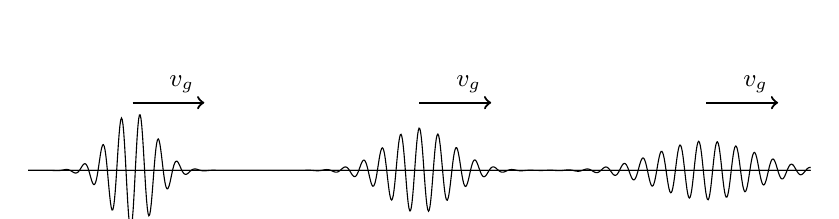
\begin{tikzpicture}
    \begin{axis}[
        width=0.95\textwidth, height=3.6cm,
        axis lines=none,
        xmin=0, xmax=12, ymin=-1.35, ymax=1.35,
        samples=1000, domain=0:12,
        clip=false,
      ]
      \addplot[black, thin] {exp(-((x-1.6)/0.5)^2)*cos(deg(22*x))};
      \addplot[black, thin] {0.72*exp(-((x-6.0)/0.72)^2)*cos(deg(22*x))};
      \addplot[black, thin] {0.50*exp(-((x-10.4)/1.05)^2)*cos(deg(22*x))};
      \draw[->,thick] (axis cs:1.6,1.15) -- (axis cs:2.7,1.15)
        node[above left]{\small $v_g$};
      \draw[->,thick] (axis cs:6.0,1.15) -- (axis cs:7.1,1.15)
        node[above left]{\small $v_g$};
      \draw[->,thick] (axis cs:10.4,1.15) -- (axis cs:11.5,1.15)
        node[above left]{\small $v_g$};
    \end{axis}
  \end{tikzpicture}
  \caption*{\small Déformation d'une onde réelle (quasi-monochromatique) dans un
  milieu dispersif: the packet travels at $v_g$ while spreading, because its
  components travel at different vitesses de phase.}
\end{figure}

\begin{definition}[Longueur d'onde]
  \[
    \lambda = \frac{2\pi}{k} = \frac{v_\varphi}{f},
    \qquad f = \frac{\omega}{2\pi}.
  \]
  Dans le cas où $\varepsilon_r = 1$, la vitesse de phase $v_\varphi = c$ et
  $\lambda = c/f$, which recovers the $\lambda = c/(f\sqrt{\varepsilon_r})$
  written earlier.
\end{definition}

\subsubsection{Impédance d'onde}

\begin{definition}[Impédance d'onde (\textit{wave impedance})]
  L'impédance d'onde $\eta$ est le rapport
  $\|\v{E}(z,t)\| \big/ \|\v{H}(z,t)\|$. Dans le cas d'une OPPM, cette
  impédance d'onde s'écrit :
  \[
    \eta = \frac{\|\v{E}_+(z)\|}{\|\v{H}_+(z)\|}
         = \frac{\omega\mu}{k}
         = \sqrt{\frac{\mu}{\varepsilon}}.
  \]
\end{definition}

Pour un milieu MLHI diélectrique avec $\mu_r = 1$ :
\[
  \eta = \sqrt{\frac{\mu_0}{\varepsilon_0\varepsilon_r}},
  \qquad\text{and for }\varepsilon_r = 1,\qquad
  \eta_0 = \sqrt{\frac{\mu_0}{\varepsilon_0}} = 120\pi\ \Omega \approx 377\ \Omega,
\]
$\eta_0$ étant l'impédance caractéristique de l'air assimilée au vide.

\begin{remark}
  One can go one step further and identify the impédance d'onde of an OPPM
  with the \textbf{impédance caractéristique du milieu de propagation}:
  \[
    Z_c = \eta = \sqrt{\frac{\mu_0}{\varepsilon_0\varepsilon_r}}.
  \]
  C'est une analogie avec la théorie des lignes de propagation autorisant un
  mode TEM --- the same $377\ \Omega$ that will reappear in the Friis bilan de
  liaison and in every antenne impedance discussion. Keep
  $377\ \Omega = 120\pi\ \Omega$ memorised; it is the single most quoted number
  of the module.
\end{remark}

\begin{example}
  In air, $\varepsilon_r \approx 1$, so $v_\varphi \approx c$ and at $f = 1$ GHz
  one gets $\lambda = 30$ cm, $k_z = 2\pi/0.30 \approx 20.9$
  $\text{rad}\cdot\text{m}^{-1}$ and $\eta \approx 377\ \Omega$.
\end{example}

\subsection{Puissance d'une OPPM dans un MLHI --- vecteur de Poynting}

\begin{definition}[Vecteur de Poynting (\textit{Poynting vector})]
  Le vecteur de Poynting, noté $\v{\Pi}$, est un vecteur dont la direction
  indique, dans un milieu MLHI, la direction de propagation d'une onde
  électromagnétique et dont l'intensité vaut la \textbf{densité de puissance}
  (\textit{power density}) véhiculée par cette onde. Le module de ce vecteur
  est donc une puissance par unité de surface ($\text{W}\cdot\text{m}^{-2}$).
  L'expression la plus générale du vecteur de Poynting est :
  \[
    \v{\Pi} = \v{E}(z,t) \wedge \v{H}(z,t).
  \]
\end{definition}

\begin{prop}[Moyenne temporelle en régime harmonique]
  Dans le cas d'une OPPM en régime harmonique, la \textbf{moyenne temporelle}
  (\textit{time average}) sur une période $T$ du vecteur de Poynting vaut :
  \[
    \langle \v{\Pi} \rangle_T
      = \tfrac{1}{2}\,\Re\!\big(\v{E}(z,t) \wedge \v{H}^{*}(z,t)\big),
  \]
  où $\v{H}^{*}(z,t)$ désigne le conjugué de $\v{H}(z,t)$.
\end{prop}

The factor $\tfrac{1}{2}$ is the usual one from averaging $\cos^2$ over a
period; the conjugation is what removes the $e^{2j\omega t}$ term and leaves a
time-independent real part.

\begin{theorem}[Puissance électromagnétique à travers une surface]
  Le flux du vecteur de Poynting à travers une surface $S$ (fermée ou non) est
  égal à la puissance véhiculée par l'onde à travers cette surface. On définit
  alors la \textbf{puissance électromagnétique} (\textit{electromagnetic power})
  de la manière suivante :
  \[
    \text{Puissance} = \iint_S \langle \v{\Pi} \rangle_T \cdot d\v{S}
      = \frac{1}{2}\,\Re\left(
          \iint_S \big(\v{E}(z,t) \wedge \v{H}^{*}(z,t)\big)\cdot d\v{S}
        \right).
  \]
\end{theorem}

Pour le cas d'une OPPM dont le champ électromagnétique est défini par les
champs établis plus haut et la définition de l'impédance d'onde $\eta$, on
écrit alors :
\[
  \v{E}(z,t) = E_+\,e^{\,j(\omega t - k_z z)}\,\v{u}_1,
  \qquad
  \v{H}(z,t) = \frac{E_+}{\eta}\,e^{\,j(\omega t - k_z z)}\,\v{u}_2,
  \qquad
  \v{u}_1 \perp \v{u}_2 \perp \v{k}_z,
\]
(rappel : pas de composante suivant $OZ$). Then
$\v{E}\wedge\v{H}^{*} = (E_+^{\,2}/\eta)\,\v{u}_1\wedge\v{u}_2$ is real and
directed along $OZ$, and

\begin{conclusion}[Puissance d'une OPPM sur une surface $S$]
  Sous condition d'onde plane sur $S$,
  \[
    \boxed{\ \text{Puissance} = \frac{E_+^{\,2}}{2\eta}\left(\iint_S d\v{S}\right)\ }
  \]
\end{conclusion}

\begin{remark}
  The two fields carry distinct unit vectors of the system $\v{u}$,
  $\v{u}_1 \perp \v{u}_2 \perp \v{k}_z$. The perpendicular pair is what makes
  the cross product non-zero and so yields the power formula above.
\end{remark}

\begin{remark}
  The form $E_+^{\,2}/2\eta$ is the field analogue of $V^2/2Z$ for an adapté
  line, and it is the quantity that the chapter on antennes integrates over a
  sphere to define puissance totale rayonnée, directivité and gain. Note that
  the power scales with the \emph{square} of the field amplitude and inversely
  with the impédance d'onde --- a medium with larger $\varepsilon_r$ has
  smaller $\eta$ and so carries more power for the same $E_+$.
\end{remark}

\subsection{La chaîne, de bout en bout}

\begin{conclusion}[What the whole part reduces to]
  Given a medium ($\varepsilon_r$, with $\mu_r = 1$, $\sigma = 0$, $\rho = 0$)
  and a source ($\omega = 2\pi f$), everything follows in one pass:
  \[
    \begin{array}{r@{\ }c@{\ }l@{\qquad}l}
      k_z &=& \omega\sqrt{\mu_0\varepsilon_0\varepsilon_r}
        & \text{dispersion equation} \\[4pt]
      v_\varphi &=& \dfrac{\omega}{k_z} = \dfrac{c}{\sqrt{\varepsilon_r}}
        & \text{phase velocity} \\[8pt]
      \lambda &=& \dfrac{2\pi}{k_z} = \dfrac{v_\varphi}{f}
                = \dfrac{c}{f\sqrt{\varepsilon_r}}
        & \text{wavelength} \\[8pt]
      \eta &=& \sqrt{\dfrac{\mu_0}{\varepsilon_0\varepsilon_r}}
             = \dfrac{\eta_0}{\sqrt{\varepsilon_r}},
             \quad \eta_0 = 120\pi \approx 377\ \Omega
        & \text{wave impedance} \\[10pt]
      \text{Puissance} &=& \dfrac{E_+^{\,2}}{2\eta}\displaystyle\iint_S d\v{S}
        & \text{power through } S
    \end{array}
  \]
  The fields themselves are $\v{E}(z,t) = \v{E}_+(z)e^{j(\omega t - k_z z)}$
  and $\v{H}(z,t) = \v{H}_+(z)e^{j(\omega t - k_z z)}$, transverse, mutually
  orthogonal, in a trièdre direct with $\v{k}$. A regressive term
  $e^{+jk_z z}$ appears only when something sends energy back --- which is
  exactly what a mismatched load on a ligne de transmission does.
\end{conclusion}

\section{Propagation sur les lignes de transmission}
Dans le cas des signaux basses fréquences (BF) utilisés dans les circuits
électroniques, la longueur d'onde $\lambda = c/f$ est extrêmement grande
($\lambda = 30$~km à 1~kHz). A circuit BF can therefore be treated as a set of
éléments localisés joined by ideal wires: dans l'approche de l'électronique BF,
la tension aux bornes de la charge est considérée égale à la tension de la
source de manière instantanée. At radio frequency this fails. Pour les signaux
radiofréquences (RF), la longueur d'onde est petite ($\lambda = 30$~cm à 1~GHz
et 3~mm à 100~GHz) et par conséquent, la taille des composants électroniques,
la longueur des pistes sur les circuits imprimés et la longueur des câbles
deviennent alors non négligeables par rapport à $\lambda$. L'importance de la
valeur relative de $\lambda$ (par rapport aux dimensions globales des circuits)
explique ainsi la raison pour laquelle les circuits RF ne peuvent pas être
traités de la même manière que les circuits BF en termes d'analyse, de
conception, de fabrication et de caractérisation. La théorie des lignes de
transmission s'applique alors aux pistes, aux câbles et plus généralement aux
circuits et systèmes RF.

\subsection{Définition d'une ligne de transmission}
\begin{definition}[Ligne de transmission (\textit{transmission line})]
  Le terme de \textbf{ligne de transmission} s'applique à certains éléments
  utilisés en ingénierie RF dont les dimensions sont du même ordre de grandeur
  que la longueur d'onde $\lambda$. Il existe différents types de lignes de
  transmission, qui se distinguent par le nombre de conducteurs métalliques
  qu'elles comportent (1, 2 ou 3 conducteurs métalliques).
\end{definition}

\subsubsection{Lignes de transmission à 1 conducteur métallique}
Les lignes comportant 1 unique conducteur métallique sont les \textbf{guides
d'ondes} (\textit{waveguide}) métalliques, qui peuvent être de forme
rectangulaire ou circulaire. Parmi les différents types de lignes de
transmission utilisées en ingénierie RF, les guides d'ondes présentent le plus
\emph{faible} affaiblissement et supportent la plus \emph{forte} puissance : ils
sont donc les mieux adaptés aux applications où l'affaiblissement des signaux
devient très élevé (typiquement, aux fréquences supérieures à 30~GHz), dans les
radars civils ou militaires, les communications satellites et les systèmes RF.
Les guides d'ondes sont de fait employés dans des situations qui ne seront pas
étudiées dans ce cours.

\subsubsection{Lignes de transmission à 2 conducteurs métalliques}
Les lignes comportant 2 conducteurs métalliques sont principalement les
\textbf{câbles coaxiaux} (\textit{coaxial cable}) et les lignes sur circuits
imprimés appelées \textbf{lignes microruban} (\textit{microstrip line}) ou
lignes microstrip. Les 2 conducteurs métalliques sont séparés par un matériau
diélectrique caractérisé par sa permittivité relative $\varepsilon_r$ (ou
constante diélectrique). La perméabilité relative est $\mu_r = 1$.

Pour un câble coaxial, le conducteur interne transporte le signal RF tandis que
le conducteur externe est la référence connectée à la masse (notée GND). Pour
une ligne microruban, c'est le conducteur supérieur qui transporte le signal RF
tandis que le conducteur inférieur constitue le \textbf{plan de masse}
(\textit{ground plane}). Les câbles coaxiaux et les lignes microruban sont les
lignes de transmission les plus fréquemment utilisées en ingénierie RF et par
conséquent, il est fondamental d'étudier leurs propriétés et caractéristiques.

\begin{example}[Diélectriques typiques]
  Un câble coaxial ayant pour matériau diélectrique du Téflon a
  $\varepsilon_r = 2{,}1$ ; le Téflon est en fait une marque déposée qui
  correspond au PolyTétraFluoroÉthylène (PTFE). Un filtre passe-bas (LPF)
  entièrement réalisé avec des lignes microruban gravées sur de l'Alumine a
  $\varepsilon_r = 9{,}8$. Dans ces 2 exemples, les conducteurs métalliques sont
  constitués de cuivre.
\end{example}

\paragraph{Câble coaxial}
Dans un câble coaxial, les champs $\v{E}$ et $\v{H}$ sont orthogonaux entre eux
et sont également orthogonaux à la direction de propagation : on retrouve alors
le mode de propagation TEM (transverse électrique et magnétique). Puisque les
champs se propagent uniquement \emph{à l'intérieur} du câble coaxial, le
rayonnement de puissance est fortement limité vers l'extérieur. Par défaut, on
dira qu'il est donc isolé d'un point de vue électromagnétique : c'est le
\textbf{blindage électromagnétique} (\textit{electromagnetic shielding}). Un
câble coaxial peut donc être facilement utilisé à proximité d'autres câbles
coaxiaux, d'un appareil de mesure, d'une surface métallique, être posé au sol,
tenu dans une main, sans interférences de la propagation du signal RF dans le
câble.

\paragraph{Ligne microstrip}
Pour les lignes microruban, les champs se propagent à la fois dans le matériau
diélectrique et dans l'air : le milieu de propagation est donc
\textbf{inhomogène} (\textit{inhomogeneous}). Les champs $\v{E}$ et $\v{H}$
possèdent une faible composante longitudinale (c'est-à-dire, le long de la
direction de propagation) : c'est le mode de propagation \textbf{quasi-TEM}.
Cependant, les composantes longitudinales des champs sont si faibles que l'on
peut considérer que le mode de propagation est TEM.

Puisque les champs se propagent en partie dans l'air, les lignes microruban ont
donc tendance à rayonner de la puissance vers l'extérieur, contrairement aux
câbles coaxiaux. Cette propriété peut être vue comme un avantage ou un
inconvénient. Le rayonnement des lignes microruban permet de les utiliser pour
concevoir des \emph{antennes} microruban ; mais pour les \emph{circuits} RF,
cela devient un inconvénient car la puissance rayonnée est alors diffusée dans
l'air, ce qui entraîne un affaiblissement plus important par rapport à un câble
coaxial de même longueur ainsi que la perturbation potentielle du fonctionnement
d'autres circuits situés à proximité.

\begin{figure}[h!]
  \centering
  \begin{tikzpicture}[scale=1.0]
    % coaxial cross-section
    \begin{scope}
      \fill[gray!10] (0,0) circle (1.3);
      \draw[very thick] (0,0) circle (1.3);
      \draw[very thick,fill=gray!50] (0,0) circle (0.3);
      \foreach \ang in {30,120,210,300}
        {\draw[->,thick] (\ang:0.32) -- (\ang:1.26);}
      \draw[dashed,gray] (0,0) circle (0.85);
      \draw[->,thick,gray] (75:0.85) arc (75:35:0.85);
      \draw[->,thick,gray] (255:0.85) arc (255:215:0.85);
      \draw[|<->|] (0,-1.6) -- node[below,font=\scriptsize,inner sep=1pt] {$b$} (-1.3,-1.6);
      \draw[|<->|] (0,-1.6) -- (0.3,-1.6);
      \node[font=\scriptsize,anchor=west,inner sep=2pt] at (0.34,-1.6) {$a$};
      \draw[gray,thin] (0,-1.3) -- (0,-1.68);
      \node[font=\scriptsize,anchor=west] at (1.45,0.75) {$\v{E}$ radial};
      \node[font=\scriptsize,anchor=west] at (1.45,0.25) {$\v{H}$ azimutal};
      \node[font=\scriptsize] at (0.62,-0.32) {$\varepsilon,\mu$};
      \node[font=\scriptsize,align=center] at (0,-2.4)
        {câble coaxial : TEM,\\ blindage électromagnétique};
    \end{scope}
    % microstrip cross-section
    \begin{scope}[xshift=6.6cm,yshift=-0.35cm]
      \fill[gray!10] (-1.7,0) rectangle (1.7,0.8);
      \draw (-1.7,0) rectangle (1.7,0.8);
      \draw[very thick,fill=gray!50] (-0.4,0.8) rectangle (0.4,0.96);
      \draw[very thick] (-1.7,0) -- (1.7,0);
      \draw[thick] (0.4,0.88) .. controls (1.0,0.88) and (1.1,0.5) .. (1.1,0);
      \draw[thick] (0.4,0.96) .. controls (1.35,1.25) and (1.6,0.6) .. (1.6,0);
      \draw[thick] (-0.4,0.88) .. controls (-1.0,0.88) and (-1.1,0.5) .. (-1.1,0);
      \draw[thick] (-0.4,0.96) .. controls (-1.35,1.25) and (-1.6,0.6) .. (-1.6,0);
      \node[font=\scriptsize] at (0,0.4) {$\varepsilon_r,\ \mu_r=1$};
      \node[font=\scriptsize,anchor=south] at (0,1.3) {air};
      \node[font=\scriptsize,anchor=south] at (0,1.0) {conducteur (signal RF)};
      \node[font=\scriptsize,anchor=north] at (0,-0.08) {plan de masse (GND)};
      \node[font=\scriptsize,align=center] at (0,-2.05)
        {ligne microruban : quasi-TEM,\\ milieu inhomogène, rayonnement};
    \end{scope}
  \end{tikzpicture}
  \caption*{\small Cross-sections of the two lignes à 2 conducteurs. In the
  câble coaxial the radial $\v{E}$ and the azimuthal $\v{H}$ are entirely
  confined between the conducteurs; in the ligne microruban part of the field
  closes through the air.}
\end{figure}

\subsection{Modèle électrique d'une ligne de transmission}
Une ligne microruban ou un câble coaxial peuvent être modélisés à l'aide d'un
circuit électrique équivalent composé d'éléments résistif $R$, inductif $L$,
conductif $G$ et capacitif $C$. Ce circuit équivalent, dit \textbf{modèle
électrique ou RLGC}, possède une longueur considérée comme quasi nulle,
$dz \to 0$, et par conséquent, une ligne de transmission de longueur $L$ est
modélisée par une infinité de circuits RLGC en cascade.

\begin{notation}
  Étant donné que $dz \to 0$, les éléments $R$, $L$, $G$, $C$ sont des
  \textbf{éléments distribués} (\textit{distributed elements}), par opposition
  à des \textbf{éléments localisés} (\textit{lumped elements}) : ils sont
  définis \emph{par unité de longueur}.
  \begin{center}
    \begin{tabular}{llll}
      \toprule
      $R$ & résistance par unité de longueur  & $\Omega/\mathrm{m}$ & pertes métalliques\\
      $L$ & inductance par unité de longueur  & $\mathrm{H}/\mathrm{m}$ & magnetic energy\\
      $G$ & conductance par unité de longueur & $\mathrm{S}/\mathrm{m}$ & pertes diélectriques\\
      $C$ & capacité par unité de longueur & $\mathrm{F}/\mathrm{m}$ & electric energy\\
      \bottomrule
    \end{tabular}
  \end{center}
\end{notation}

La résistance par unité de longueur $R$ est due à la conductivité $\sigma$ non
infinie (ou la résistivité $\rho = 1/\sigma$ non nulle) des conducteurs
métalliques de la ligne de transmission. L'inductance par unité de longueur $L$
modélise le fait qu'un courant qui circule dans un conducteur métallique crée
un champ magnétique. La capacité par unité de longueur $C$ s'explique par le
fait qu'il y a 2 conducteurs métalliques à un potentiel différent et séparés
par un matériau diélectrique : il existe donc un champ électrique entre les 2
conducteurs métalliques. Les matériaux diélectriques isolants ne sont pas
parfaitement isolants et ils présentent des pertes. Ces pertes dans les
matériaux diélectriques sont modélisées par la conductance par unité de
longueur $G$.

\begin{prop}[Ligne sans pertes (\textit{lossless line})]
  Les éléments $R$ et $G$ du modèle équivalent sont responsables des pertes
  (atténuation notée $\alpha$) dans les lignes microruban et les câbles
  coaxiaux : $R$ est à l'origine des pertes dans les conducteurs métalliques,
  tandis que $G$ est à l'origine des pertes dans le matériau diélectrique.
  Ainsi, il est souhaitable pour une ligne de transmission de présenter une
  faible résistance par unité de longueur $R$ et une faible conductance par
  unité de longueur $G$, et
  \[\text{\textbf{lossless (ideal) line}} \iff R = 0 \text{ and } G = 0.\]
\end{prop}

\begin{remark}[Why copper, and why Teflon or air]
  Le cuivre ($\sigma = 58{,}7\times 10^{6}$~S/m) et l'aluminium
  ($\sigma = 36{,}9 \times 10^{6}$~S/m), qui font partie des métaux ayant la
  conductivité la plus élevée, sont presque exclusivement utilisés comme
  conducteur métallique dans les lignes microruban et les câbles coaxiaux. L'or
  est également un très bon conducteur ($\sigma = 41 \times 10^{6}$~S/m) mais
  le prix est bien trop élevé pour être massivement utilisé dans les câbles et
  circuits RF. Quant au choix du matériau diélectrique, il est fonction de
  nombreux paramètres et n'est pas uniquement guidé par la recherche de pertes
  diélectriques minimales. Si en pratique ce choix est assez vaste pour les
  lignes microruban, il est beaucoup plus limité pour les câbles coaxiaux où le
  Téflon ($\tan\delta = 5\times 10^{-4}$) et l'air ($\tan\delta = 0$) sont
  principalement utilisés. L'air sec est ainsi le matériau diélectrique qui
  présente les plus faibles pertes et il est systématiquement présent dans les
  câbles coaxiaux fonctionnant à des fréquences supérieures à environ 25~GHz.
\end{remark}

\begin{figure}[h!]
  \centering
  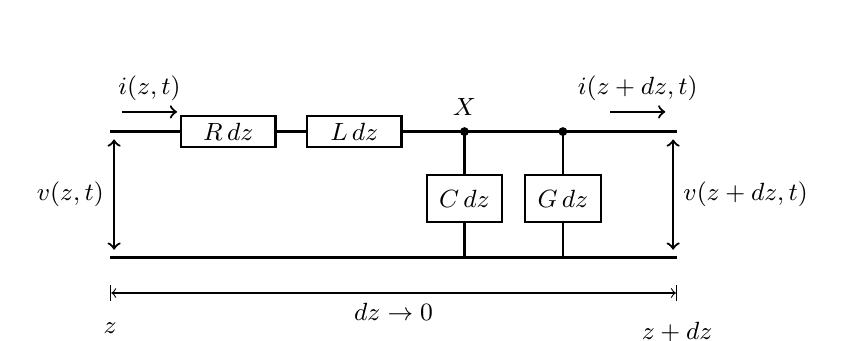
\begin{tikzpicture}[scale=1.0]
    % top wire with R dz and L dz
    \draw[thick] (-1.2,1.6) -- (-0.3,1.6);
    \draw[thick,fill=white] (-0.3,1.4) rectangle (0.9,1.8);
    \node[font=\small] at (0.3,1.6) {$R\,dz$};
    \draw[thick] (0.9,1.6) -- (1.3,1.6);
    \draw[thick,fill=white] (1.3,1.4) rectangle (2.5,1.8);
    \node[font=\small] at (1.9,1.6) {$L\,dz$};
    \draw[thick] (2.5,1.6) -- (6.0,1.6);
    % shunt branches
    \draw[thick] (3.3,1.6) -- (3.3,1.05);
    \draw[thick,fill=white] (2.82,0.45) rectangle (3.78,1.05);
    \node[font=\small] at (3.3,0.75) {$C\,dz$};
    \draw[thick] (3.3,0.45) -- (3.3,0.0);
    \draw[thick] (4.55,1.6) -- (4.55,1.05);
    \draw[thick,fill=white] (4.07,0.45) rectangle (5.03,1.05);
    \node[font=\small] at (4.55,0.75) {$G\,dz$};
    \draw[thick] (4.55,0.45) -- (4.55,0.0);
    \fill (3.3,1.6) circle (1.6pt);
    \fill (4.55,1.6) circle (1.6pt);
    \node[font=\small,anchor=south] at (3.3,1.68) {$X$};
    % bottom wire
    \draw[thick] (-1.2,0.0) -- (6.0,0.0);
    % ports
    \draw[->,thick] (-1.05,1.85) -- (-0.35,1.85);
    \node[font=\small,anchor=south] at (-0.7,1.87) {$i(z,t)$};
    \draw[->,thick] (5.15,1.85) -- (5.85,1.85);
    \node[font=\small,anchor=south] at (5.5,1.87) {$i(z+dz,t)$};
    \draw[<->,thick] (-1.15,1.5) -- node[left,font=\small] {$v(z,t)$} (-1.15,0.1);
    \draw[<->,thick] (5.95,1.5) -- node[right,font=\small] {$v(z+dz,t)$} (5.95,0.1);
    % axis
    \draw[|<->|] (-1.2,-0.45) -- node[below,font=\small] {$dz \to 0$} (6.0,-0.45);
    \node[font=\small,anchor=north] at (-1.2,-0.7) {$z$};
    \node[font=\small,anchor=north] at (6.0,-0.7) {$z+dz$};
  \end{tikzpicture}
  \caption*{\small The elementary RLGC cell. The loi des mailles is applied to
  the loop, the loi des nœuds to the nœud between the series and the shunt
  branch.}
\end{figure}

\subsubsection{Les éléments L et C pour un câble coaxial sans perte}
Pour un câble coaxial, les champs restent confinés à l'intérieur du câble et la
section droite du câble possède une symétrie circulaire. Pour ces raisons, les
éléments $L$ et $C$ peuvent être calculés analytiquement et les expressions
obtenues sont relativement simples. Ils dépendent à la fois de grandeurs
physiques $(\varepsilon,\mu)$ et de paramètres géométriques, avec $a$ le rayon
du conducteur interne et $b$ le rayon du conducteur externe :
\[
  L = \frac{\mu}{2\pi}\ln\!\left(\frac{b}{a}\right),
  \qquad
  C = \frac{2\pi\varepsilon}{\ln(b/a)}.
\]

\subsubsection{L et C pour une ligne microstrip sans pertes}
Pour une ligne microruban, les champs se propagent à la fois dans le matériau
diélectrique et dans l'air et de plus, la section droite de la ligne ne possède
aucune symétrie. Pour ces raisons, il n'existe \emph{pas} de relations
analytiques simples pour définir $R$, $L$, $G$, $C$ pour une ligne microruban.
Les éléments sont alors déterminés par mesures de caractérisation et on définit
ainsi le modèle électrique équivalent RLGC.

\subsection{Équation des télégraphistes}
Une ligne de transmission à 2 conducteurs peut être modélisée par une infinité
de circuits équivalents RLGC identiques mis en cascade ; il suffit alors d'en
analyser un seul pour en déduire les caractéristiques de l'ensemble de la ligne
de transmission. L'application de la théorie des circuits est utilisée.
Celle-ci est basée sur les 2 lois de Kirchhoff, aussi connues sous le nom de
\textbf{loi des mailles} (\textit{Kirchhoff's voltage law}) et de \textbf{loi
des nœuds} (\textit{Kirchhoff's current law}). La loi des mailles énonce que la
somme des tensions dans une maille $ABCD$ est nulle et la loi des nœuds énonce
que la somme des courants entrant et sortant au niveau d'un nœud $X$ est nulle.

Around the loop,
$v(z,t) - R\,dz\,i(z,t) - L\,dz\,\frac{\partial i(z,t)}{\partial t}
- v(z+dz,t) = 0$; at the nœud,
$i(z,t) - G\,dz\,v(z+dz,t) - C\,dz\,\frac{\partial v(z+dz,t)}{\partial t}
- i(z+dz,t) = 0$. Dividing by $dz$ and letting $dz \to 0$, on obtient les
\textbf{équations des télégraphistes} (\textit{telegrapher's equations}) en
régime général (in the time domain) :
\begin{align}
  -\frac{\partial v(z,t)}{\partial z}
    &= R\, i(z,t) + L\,\frac{\partial i(z,t)}{\partial t} \tag{1}\\
  -\frac{\partial i(z,t)}{\partial z}
    &= G\, v(z,t) + C\,\frac{\partial v(z,t)}{\partial t} \tag{2}
\end{align}

\begin{remark}
  The right-hand sides of (1) and (2) carry the time derivatives
  $\partial i/\partial t$ and $\partial v/\partial t$; the spatial derivatives
  $\partial i/\partial z$ and $\partial v/\partial z$ appear only on the
  left-hand sides. Every use made of the equations afterwards rests on the time
  derivatives.
\end{remark}

En \textbf{régime harmonique} (\textit{harmonic regime}), $v(z,t)$ et $i(z,t)$
sont définies par les fonctions sinusoïdales
\begin{align}
  v(z,t) &= \Re\!\left(V(z)\,e^{j\omega t}\right) \tag{3}\\
  i(z,t) &= \Re\!\left(I(z)\,e^{j\omega t}\right) \tag{4}
\end{align}
L'étude comportementale de la ligne de transmission en régime harmonique ne va
dépendre que de la dépendance spatiale de la ligne décrite par $V(z)$ et
$I(z)$, représentant la tension et le courant au point d'abscisse $z$ sur la
ligne. Le terme $e^{j\omega t}$ est toujours présent dans $v(z,t)$ et $i(z,t)$
mais inutile pour caractériser la ligne de transmission --- it is dropped from
here on.

En injectant (3) dans (1) et (4) dans (2), on obtient alors les équations des
télégraphistes en régime harmonique :
\begin{align}
  -\frac{dV(z)}{dz} &= (R + j\omega L)\, I(z) \tag{5}\\
  -\frac{dI(z)}{dz} &= (G + j\omega C)\, V(z) \tag{6}
\end{align}

Pour obtenir les équations de cette ligne de transmission, il faut exprimer (5)
et (6) en fonction d'une seule variable, en les dérivant une seconde fois en
fonction de $z$ : en dérivant (5) et en y introduisant (6), puis en dérivant
(6) et en y introduisant (5), on obtient
\[
  \frac{d^2V(z)}{dz^2} - (R+j\omega L)(G+j\omega C)\,V(z) = 0,
  \qquad
  \frac{d^2I(z)}{dz^2} - (R+j\omega L)(G+j\omega C)\,I(z) = 0 .
\]

\begin{theorem}[Équations des lignes de transmission]
  En posant $\gamma = \sqrt{(R+jL\omega)(G+jC\omega)}$, on peut écrire les
  \textbf{équations des lignes de transmission} (\textit{transmission-line
  equations}) :
  \[
    \boxed{\;\frac{d^2V(z)}{dz^2} - \gamma^2 V(z) = 0,
    \qquad
    \frac{d^2I(z)}{dz^2} - \gamma^2 I(z) = 0. \;}
  \]
\end{theorem}

\begin{remark}
  Mêmes équations différentielles mais adaptées aux courants et tensions ---
  the same equations as for an onde électromagnétique plane. Pour une onde EM,
  on utilisera $k$ ; pour une ligne de transmission, on utilise $\gamma$.
\end{remark}

\subsection{Constante de propagation complexe $\gamma$}
\begin{definition}[Constante de propagation complexe]
  La \textbf{constante de propagation complexe} (\textit{complex propagation
  constant}) d'une ligne de transmission s'écrit
  \[
    \gamma = \sqrt{(R+j\omega L)(G+j\omega C)} = \alpha + j\,\beta .
  \]
  Sa partie réelle $\alpha$ est appelée \textbf{constante d'atténuation}
  (\textit{attenuation constant}) : $V(z)$ et $I(z)$ sont atténués le long de
  la ligne de propagation. Sa partie imaginaire $\beta$ est appelée
  \textbf{constante de phase} (\textit{phase constant}) : $V(z)$ et $I(z)$
  subissent un \textbf{déphasage} (\textit{phase shift}) le long de la ligne de
  propagation.
\end{definition}

Separating real and imaginary parts, on identifie alors $\alpha$ et $\beta$ :
\[
  \alpha = \left[\tfrac{1}{2}\left\{
    \sqrt{\left[R^2 + (L\omega)^2\right]\left[G^2 + (C\omega)^2\right]}
    + RG - LC\omega^2 \right\}\right]^{1/2},
\]
\[
  \beta = \left[\tfrac{1}{2}\left\{
    \sqrt{\left[R^2 + (L\omega)^2\right]\left[G^2 + (C\omega)^2\right]}
    - RG + LC\omega^2 \right\}\right]^{1/2}.
\]

\begin{remark}
  The two lines differ only in the sign of the last term: $\beta$ carries
  $-(RG - LC\omega^2)$ where $\alpha$ carries $+(RG - LC\omega^2)$, i.e.\
  $-RG + LC\omega^2$ inside the $\beta$ line. Setting $R = G = 0$ in it
  recovers the lossless value $\beta = \omega\sqrt{LC}$ stated below. The two
  special cases used in this course are $\alpha = 0$ and
  $\beta = \omega\sqrt{LC}$.
\end{remark}

\begin{corollary}[Ligne sans pertes]
  Dans le cas d'une ligne de transmission sans pertes, $R = G = 0$, et donc
  \[
    \alpha = 0, \qquad \beta = \omega\sqrt{LC}, \qquad \gamma = j\beta .
  \]
\end{corollary}

Il est intéressant de remarquer que $\alpha$ et $\beta$ dépendent de la
pulsation $\omega$ et donc de la fréquence $f$, avec $\omega = 2\pi f$. For a
ligne sans pertes the constante de phase fixes the longueur d'onde on the line:
\[
  \beta = \omega\sqrt{LC} = \frac{2\pi}{\lambda},
  \qquad \lambda = \frac{c}{f\sqrt{\varepsilon_r}} .
\]
The longueur d'onde inside the line is therefore \emph{shorter} than in vacuum
by the factor $\sqrt{\varepsilon_r}$, which is why a $\lambda/4$ section of
câble coaxial with a Téflon diélectrique is physically shorter than a quarter of
the longueur d'onde in espace libre.

\subsection{Solutions générales des équations des télégraphistes}
Les équations des lignes de transmission sont des équations différentielles du
second ordre ayant respectivement pour variables la tension $V(z)$ et le
courant $I(z)$. Leurs solutions générales sont les suivantes :
\[
  V(z) = V^{+}e^{-\gamma z} + V^{-}e^{+\gamma z} = V^{+}(z) + V^{-}(z),
  \qquad
  I(z) = I^{+}e^{-\gamma z} + I^{-}e^{+\gamma z} = I^{+}(z) + I^{-}(z),
\]
où $V^{+}$, $V^{-}$, $I^{+}$, $I^{-}$ sont respectivement les amplitudes de
$V^{+}(z)$, $V^{-}(z)$, $I^{+}(z)$, $I^{-}(z)$.

\begin{definition}[Ondes incidentes et ondes réfléchies]
  Les solutions physiques des équations des lignes de transmission
  correspondent à des ondes de tension et de courant qui se propagent en sens
  \emph{opposés}. $V^{+}(z)$ et $I^{+}(z)$ se propagent dans le sens des
  $z > 0$ : on les appelle les \textbf{ondes incidentes} (\textit{incident
  wave}), du générateur vers l'impédance de charge $Z_L$. $V^{-}(z)$ et
  $I^{-}(z)$ se propagent dans le sens des $z < 0$ : ce sont les \textbf{ondes
  réfléchies} (\textit{reflected wave}), de la charge vers le générateur.
\end{definition}

Si on introduit l'expression de $\gamma = \alpha + j\beta$ dans les solutions
générales, on obtient les relations suivantes, where each term splits into a
real attenuation factor and a complex phase factor:
\[
  V(z) = V^{+}e^{-\alpha z}e^{-j\beta z} + V^{-}e^{\alpha z}e^{j\beta z},
  \qquad
  I(z) = I^{+}e^{-\alpha z}e^{-j\beta z} + I^{-}e^{\alpha z}e^{j\beta z}.
\]
Ces expressions montrent bien que les termes $e^{-\alpha z}$ et $e^{\alpha z}$
sont réels et tendent à réduire l'amplitude de $V(z)$ et $I(z)$, d'où le nom de
constante d'\emph{atténuation} donné à $\alpha$. Les termes $e^{-j\beta z}$ et
$e^{j\beta z}$ sont complexes et contribuent à la rotation de la phase de
$V(z)$ et $I(z)$, d'où le nom de constante de \emph{phase} donné à $\beta$.

\begin{remark}
  Si on relève simultanément les tensions $V(0)$, $V(z)$ et $V(L)$ sur une
  ligne de longueur $L$, l'amplitude sera différente et dépendante de l'endroit
  où la tension est mesurée. Pour une ligne \emph{sans pertes}, l'amplitude
  maximale par période $\lambda$ reste inchangée ; pour une ligne \emph{avec
  pertes}, cette amplitude maximale diminue aussi en fonction de $z$.
\end{remark}

\subsection{Impédance caractéristique $Z_C$ d'une ligne de propagation}
\begin{notation}
  Dans ce cours, nous prendrons par convention l'origine $z = 0$ à l'interface
  ligne de propagation/impédance de charge $Z_L$, so that the line occupies
  $z < 0$ and a point at distance $l$ back towards the generator is at
  $z = -l$.
\end{notation}

Les équations des lignes de transmission admettent pour solutions physiques la
forme générale suivante, avec $V_0^{+}, V_0^{-}$ la tension incidente et la
tension réfléchie au point $z = 0$ :
\[
  V(z) = V_0^{+}e^{-\gamma z} + V_0^{-}e^{+\gamma z},
  \qquad
  I(z) = I_0^{+}e^{-\gamma z} + I_0^{-}e^{+\gamma z}.
\]

\begin{proof}
  En dérivant $V(z)$, on obtient
  $-\dfrac{dV(z)}{dz} = \gamma V_0^{+}e^{-\gamma z} - \gamma V_0^{-}e^{\gamma z}$,
  et, à partir de l'équation (5), ce terme est égal à $(R+j\omega L)I(z)$. En
  remplaçant $\gamma$ par $\sqrt{(R+j\omega L)(G+j\omega C)}$, on obtient
  \[
    I(z) = \sqrt{\frac{G+j\omega C}{R+j\omega L}}\,V_0^{+}e^{-\gamma z}
         - \sqrt{\frac{G+j\omega C}{R+j\omega L}}\,V_0^{-}e^{\gamma z}
         = \frac{V_0^{+}}{Z_C}e^{-\gamma z} - \frac{V_0^{-}}{Z_C}e^{\gamma z},
  \]
  avec $Z_C = \sqrt{(R+j\omega L)/(G+j\omega C)}$. \qed
\end{proof}

\begin{definition}[Impédance caractéristique (\textit{characteristic impedance})]
  Pour une ligne d'impédance caractéristique $Z_C$, on prendra pour notation
  \[
    \boxed{\;
    V(z) = V_0^{+}e^{-\gamma z} + V_0^{-}e^{+\gamma z},
    \qquad
    I(z) = \frac{V_0^{+}}{Z_C}e^{-\gamma z} - \frac{V_0^{-}}{Z_C}e^{+\gamma z},
    \;}
  \]
  avec
  \[
    \boxed{\;
    Z_C = \sqrt{\frac{R+j\omega L}{G+j\omega C}}
        = \frac{V^{+}(z)}{I^{+}(z)} = -\,\frac{V^{-}(z)}{I^{-}(z)} .
    \;}
  \]
\end{definition}

$Z_C$ est définie comme étant le rapport entre les grandeurs
\emph{progressives} $V^{+}(z)$ et $I^{+}(z)$, ou l'\emph{opposé} du rapport
entre les ondes régressives $V^{-}(z)$ et $I^{-}(z)$ --- note the minus sign,
which is exactly what makes $Z_C$ a positive quantity for a backward-travelling
wave. Le terme $Z_C$ est bien une impédance. Étant donné que les éléments $R$,
$L$, $G$, $C$ sont constants sur toute la longueur de la ligne, $Z_C$ est une
valeur constante tout le long de la ligne (pour une fréquence de signal
donnée). Ceci constitue un résultat intéressant car bien que $V^{+}(z)$ et
$I^{+}(z)$ (respectivement, $V^{-}(z)$ et $I^{-}(z)$) varient en fonction de
$z$, leur rapport ne dépend pas de $z$.

\begin{corollary}[Ligne sans pertes]
  Pour une ligne sans pertes, $R = G = 0$ :
  \[
    Z_C = \sqrt{\frac{L}{C}} .
  \]
\end{corollary}

\begin{example}[Câble coaxial]
  En prenant l'exemple du câble coaxial sans pertes, its $L$ and $C$ are
  substituted into $Z_C = \sqrt{L/C}$ : $\mu_r = 1$ et
  $\sqrt{\mu_0/\varepsilon_0} \approx 377\ \Omega$, alors
  \[
    Z_C = \sqrt{\frac{L}{C}}
        = \frac{377}{2\pi\sqrt{\varepsilon_r}}\ln\!\left(\frac{b}{a}\right)
        \approx \frac{60}{\sqrt{\varepsilon_r}}\ln\!\left(\frac{b}{a}\right).
  \]
  Le Téflon ($\varepsilon_r = 2{,}1$) est souvent utilisé comme matériau
  diélectrique dans les câbles. Les dimensions utilisées sont telles que
  $a = 1{,}4$~mm et $b = 4{,}9$~mm, et l'on obtient une valeur approximative de
  50~ohms. The outer radius that lands exactly on the standard value is
  slightly smaller:
  \[
    Z_C = \frac{60}{\sqrt{2{,}1}}\ln\!\left(\frac{4{,}69}{1{,}4}\right)
        \approx 50\ \Omega .
  \]
  Note that $Z_C$ depends only on the \emph{ratio} $b/a$ and on
  $\varepsilon_r$, not on the absolute size of the cable.
\end{example}

\begin{remark}
  With $b = 4{,}9$~mm the formula gives $\approx 52\ \Omega$: the pair
  $a = 1{,}4$~mm, $b = 4{,}9$~mm yields $Z_C \approx 50\ \Omega$ only as a
  round figure. It is $4{,}69$ that lands on $50\ \Omega$, which is why the
  chain above carries $\ln(4{,}69/1{,}4)$ rather than the ratio for
  $b = 4{,}9$~mm.
\end{remark}

\subsubsection{Pourquoi le choix de 50 ohms ?}
Cette valeur d'impédance caractéristique, $Z_C = 50\ \Omega$, a été choisie par
la Commission Électrotechnique Internationale (IEC) comme valeur de référence
(ou valeur standardisée) pour les câbles coaxiaux, les circuits RF et les
appareils de test \& mesures RF.

Ce choix résulte de la recherche d'un \textbf{compromis} entre atténuation
minimale du signal RF et puissance maximale de ce signal RF dans un câble
coaxial. L'atténuation minimale d'un signal RF est obtenue pour un câble
coaxial avec $Z_C = 77\ \Omega$, tandis que la puissance maximale transportable
est obtenue pour $Z_C = 30\ \Omega$. La valeur $50\ \Omega$ correspond
approximativement à la valeur intermédiaire entre les deux, soit
$(30+77)/2 = 53{,}5\ \Omega \approx 50\ \Omega$ : un câble coaxial de
$50\ \Omega$ présente une atténuation 10~\% supérieure par rapport à un câble
de $77\ \Omega$ et une réduction de 10~\% de la puissance maximale
transportable par rapport à un câble de $30\ \Omega$. Ce choix constitue donc
un très bon compromis.

\begin{figure}[h!]
  \centering
  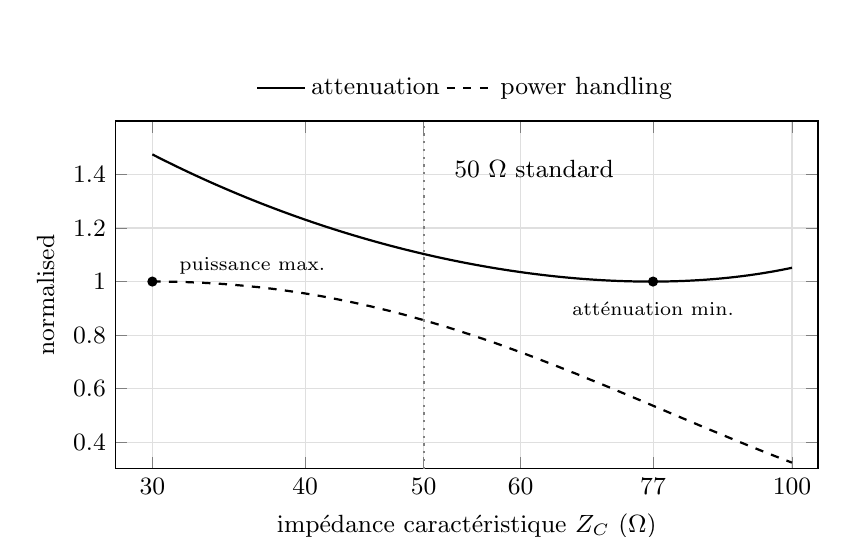
\begin{tikzpicture}
    \begin{axis}[
      width=10.5cm, height=6.0cm,
      xmode=log, log basis x=10,
      xlabel={impédance caractéristique $Z_C$ ($\Omega$)},
      ylabel={normalised},
      xmin=28, xmax=105, ymin=0.3, ymax=1.6,
      xtick={30,40,50,60,77,100},
      xticklabels={30,40,50,60,77,100},
      ytick={0.4,0.6,0.8,1.0,1.2,1.4},
      grid=both, grid style={gray!25},
      legend style={at={(0.5,1.03)},anchor=south,legend columns=2,
                    draw=none,font=\small},
      tick label style={font=\small}, label style={font=\small},
      ]
      \addplot[thick,domain=30:100,samples=90] {((1+exp(x/60))/(x/60))/3.5913};
      \addlegendentry{attenuation}
      \addplot[thick,dashed,domain=30:100,samples=90]
        {((x/60)*exp(-2*x/60))/0.18394};
      \addlegendentry{power handling}
      \draw[gray,dotted,thick] (axis cs:50,0.3) -- (axis cs:50,1.6);
      \node[font=\small,anchor=west] at (axis cs:52,1.42) {$50\ \Omega$ standard};
      \node[circle,fill=black,inner sep=1.3pt] at (axis cs:77,1.0) {};
      \node[font=\scriptsize,anchor=north] at (axis cs:77,0.96)
        {atténuation min.};
      \node[circle,fill=black,inner sep=1.3pt] at (axis cs:30,1.0) {};
      \node[font=\scriptsize,anchor=west] at (axis cs:31,1.06)
        {puissance max.};
    \end{axis}
  \end{tikzpicture}
  \caption*{\small The $50\ \Omega$ compromise for a câble coaxial:
  attenuation is minimum at $Z_C = 77\ \Omega$, power handling is maximum at
  $Z_C = 30\ \Omega$, and $50\ \Omega$ costs about 10~\% of each.}
\end{figure}

\begin{remark}[Physical meaning of $Z_C$ --- read this one twice]
  $Z_C$ n'est \emph{pas} une impédance « matérielle » mais un modèle décrivant
  la distribution de la puissance du signal progressif, à l'abscisse $z$, se
  propageant sur la ligne : cette puissance est distribuée sur la tension
  $V^{+}(z)$ et le courant $I^{+}(z)$ en fonction des dimensions transversales
  et des caractéristiques du matériau diélectrique de la ligne de propagation.
  Equivalently, $Z_C$ est l'impédance qui serait vue en $z = -l$ si la ligne
  était de longueur infinie --- ou fermée par une impédance de charge adaptée
  (c'est-à-dire qu'il n'y a pas de réflexion).
\end{remark}

\subsection{Facteur de réflexion, impédance ramenée, ondes stationnaires}
À noter que l'on va traiter exclusivement le cas de \emph{lignes sans pertes}
($\alpha = 0$, $\gamma = j\beta$) dans ce cours.

\begin{figure}[h!]
  \centering
  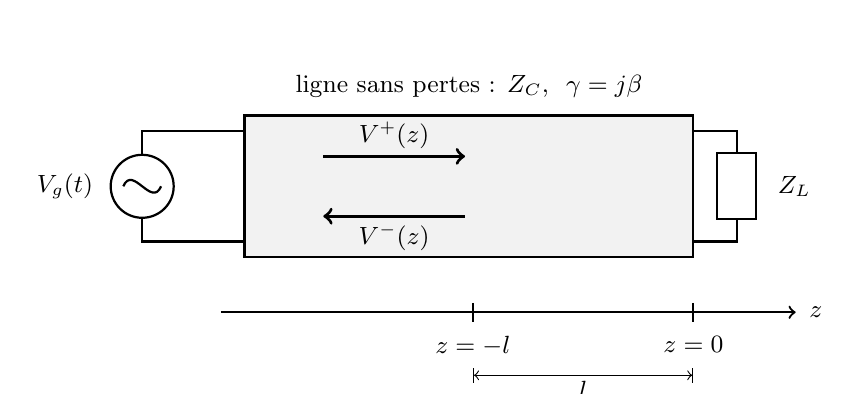
\begin{tikzpicture}[scale=1.0]
    % line body
    \fill[gray!10] (1.3,-0.9) rectangle (7,0.9);
    \draw[thick] (1.3,-0.9) rectangle (7,0.9);
    \node[font=\small,anchor=south] at (4.15,1.0)
      {ligne sans pertes : $Z_C$,\ \ $\gamma = j\beta$};
    \draw[->,very thick] (2.3,0.38) -- node[above,font=\small,inner sep=2pt]
      {$V^{+}(z)$} (4.1,0.38);
    \draw[<-,very thick] (2.3,-0.38) -- node[below,font=\small,inner sep=2pt]
      {$V^{-}(z)$} (4.1,-0.38);
    % generator
    \draw[thick] (0,0) circle (0.4);
    \draw[thick] (-0.24,0) .. controls (-0.12,0.28) and (0.12,-0.28) .. (0.24,0);
    \node[font=\small,anchor=east] at (-0.5,0) {$V_g(t)$};
    \draw[thick] (0,0.4) -- (0,0.7) -- (1.3,0.7);
    \draw[thick] (0,-0.4) -- (0,-0.7) -- (1.3,-0.7);
    % load
    \draw[thick,fill=white] (7.3,-0.42) rectangle (7.8,0.42);
    \node[font=\small,anchor=west] at (7.95,0) {$Z_L$};
    \draw[thick] (7,0.7) -- (7.55,0.7) -- (7.55,0.42);
    \draw[thick] (7,-0.7) -- (7.55,-0.7) -- (7.55,-0.42);
    % axis
    \draw[->,thick] (1.0,-1.6) -- (8.3,-1.6);
    \node[font=\small,anchor=west] at (8.35,-1.6) {$z$};
    \draw[thick] (7,-1.48) -- (7,-1.72);
    \node[font=\small,anchor=north] at (7,-1.78) {$z=0$};
    \draw[thick] (4.2,-1.48) -- (4.2,-1.72);
    \node[font=\small,anchor=north] at (4.2,-1.78) {$z=-l$};
    \draw[|<->|] (4.2,-2.4) -- node[below,font=\small,inner sep=2pt] {$l$} (7,-2.4);
  \end{tikzpicture}
  \caption*{\small The reference configuration. The origin sits at the load, so
  the line lives at $z<0$ and $z=-l$ is a distance $l$ back towards the
  generator.}
\end{figure}

\subsubsection{Facteur de réflexion}
En $z = 0$, la tension et le courant s'écrivent :
\[
  V(z=0) = V_0^{+} + V_0^{-}, \qquad
  I(z=0) = \frac{V_0^{+}}{Z_C} - \frac{V_0^{-}}{Z_C} .
\]
L'existence d'une tension et d'un courant réfléchis le long de la ligne est
dépendante d'une réflexion de l'onde incidente au niveau de l'interface
ligne/impédance de charge en $z=0$.

\begin{definition}[Facteur de réflexion]
  On peut exprimer le \textbf{facteur de réflexion} (\textit{reflection
  coefficient}) à la charge ainsi :
  \[
    \Gamma(z=0) = \frac{V_0^{-}}{V_0^{+}},
  \]
  avec $V_0^{+}$ l'amplitude de la tension incidente et $V_0^{-}$ l'amplitude
  de la tension réfléchie en $z=0$. En $z = -l$, où
  $V(z=-l) = V_0^{+}e^{-j\beta l} + V_0^{-}e^{+j\beta l}$ et
  $I(z=-l) = \left(V_0^{+}e^{-j\beta l} - V_0^{-}e^{+j\beta l}\right)/Z_C$,
  le facteur de réflexion s'écrit alors
  \[
    \Gamma(z=-l) = \frac{V_0^{-}e^{+j\beta l}}{V_0^{+}e^{-j\beta l}}
                 = \frac{V_0^{-}}{V_0^{+}}\,e^{+2j\beta l},
  \]
  et en tout point $z$ de la ligne sans pertes, on peut écrire :
  \[
    \boxed{\; \Gamma(z) = \frac{V_0^{-}}{V_0^{+}}\,e^{+2j\beta z}. \;}
  \]
\end{definition}

On notera le module $|\Gamma(z)| = |V_0^{-}|/|V_0^{+}|$ du facteur de
réflexion, constant along a ligne sans pertes; only the phase changes, and it
changes at twice the rate of a one-way trip --- the déphasage $2\beta z$
accounts for the round trip to the load and back.

\subsubsection{Expression de l'impédance le long d'une ligne ou impédance ramenée}
En $z=0$, l'impédance de charge est liée à la tension et au courant par :
\[
  Z_L = \frac{V(z=0)}{I(z=0)} = Z_C\,\frac{V_0^{+} + V_0^{-}}{V_0^{+} - V_0^{-}}
      = Z_C\,\frac{1+\Gamma(z=0)}{1-\Gamma(z=0)} .
\]

\begin{theorem}[Facteur de réflexion d'une impédance de charge]
  \[
    \boxed{\;
    \Gamma(z=0) = \frac{V_0^{-}}{V_0^{+}} = \frac{Z_L - Z_C}{Z_L + Z_C} .
    \;}
  \]
\end{theorem}

\begin{notation}[Quelques valeurs à retenir]
  Four limiting cases of $\Gamma$ at the load:
  \begin{itemize}
    \item Si $Z_L$ est un \textbf{court-circuit} (\textit{short circuit}, CC),
      $Z_L = 0$ : $\Gamma(z=0) = -1$.
    \item Si $Z_L$ est un \textbf{circuit ouvert} (\textit{open circuit}, CO),
      $Z_L = \infty$ : $\Gamma(z=0) = +1$.
    \item Si $Z_L$ est \textbf{adaptée} (\textit{matched}) à la ligne,
      $Z_L = Z_C$ : $\Gamma(z=0) = 0$ (pas de réflexion).
    \item $-1 \le \Gamma(z=0) \le 1$ (and $0 \le |\Gamma(z=0)| \le 1$ in the
      complex case).
  \end{itemize}
\end{notation}

Pour une ligne sans pertes de longueur $l$, on peut ainsi déterminer
l'\textbf{impédance ramenée} --- the impedance ``brought back'' to $z=-l$ ---
créée par l'impédance de charge $Z_L$ et le tronçon de ligne de propagation de
longueur $l$. The algebra is carried at an arbitrary abscissa $z$ and
specialised to $z=-l$ only at the very end:
\[
  Z(z) = \frac{V(z)}{I(z)}
       = Z_C\,\frac{V_0^{+}e^{-j\beta z} + V_0^{-}e^{+j\beta z}}
                   {V_0^{+}e^{-j\beta z} - V_0^{-}e^{+j\beta z}}
       = Z_C\,\frac{e^{-j\beta z} + \Gamma(z=0)\,e^{+j\beta z}}
                   {e^{-j\beta z} - \Gamma(z=0)\,e^{+j\beta z}} .
\]
En introduisant $\Gamma(z=0) = (Z_L-Z_C)/(Z_L+Z_C)$, l'expression ci-dessus
devient (after clearing the inner denominators) :
\[
  Z(z) = Z_C\,
  \frac{Z_L\left(e^{-j\beta z} + e^{+j\beta z}\right)
        + Z_C\left(e^{-j\beta z} - e^{+j\beta z}\right)}
       {Z_L\left(e^{-j\beta z} - e^{+j\beta z}\right)
        + Z_C\left(e^{-j\beta z} + e^{+j\beta z}\right)} .
\]
$Z(z) = Z_C\left(Z_L - jZ_C\tan(\beta z)\right)/\left(Z_C - jZ_L\tan(\beta z)\right)$
s'obtient en faisant apparaître l'expression des lignes trigonométriques ;
setting $z = -l$ --- which flips the sign of the sines --- gives the result to
remember.

\begin{theorem}[Impédance ramenée]
  Pour une ligne sans pertes d'impédance caractéristique $Z_C$ fermée sur une
  impédance de charge $Z_L$, l'impédance vue à l'abscisse $z = -l$ est
  \[
    \boxed{\;
    Z(z=-l) = Z_C\,
    \frac{Z_L + j\,Z_C\tan(\beta l)}{Z_C + j\,Z_L\tan(\beta l)} .
    \;}
  \]
\end{theorem}

\begin{remark}
  Carried directly in $l$, the collection step reads
  $Z_L(e^{+j\beta l} + e^{-j\beta l}) + Z_C(e^{+j\beta l} - e^{-j\beta l})$
  over $Z_L(e^{+j\beta l} - e^{-j\beta l}) + Z_C(e^{+j\beta l} + e^{-j\beta l})$:
  at $z = -l$ the two exponentials of the route in $z$ swap places, and the
  term in $Z_C$ enters the denominator with a plus sign. Both routes close on
  the box.
\end{remark}

\begin{corollary}[Ligne quart d'onde (\textit{quarter-wave line})]
  Ici $\beta = 2\pi/\lambda$, et une ligne de longueur $l = \lambda/4$ donne
  $\beta l = \pi/2$ et $\tan(\beta l) \to \infty$, d'où l'impédance ramenée
  \[
    \boxed{\; Z(z=-\lambda/4) = \frac{Z_C^{\,2}}{Z_L} . \;}
  \]
  Il s'agit d'un \textbf{transformateur d'impédance} (\textit{impedance
  transformer}). Ce cas particulier sera utilisé au chapitre suivant traitant
  de l'adaptation d'impédance --- it is the basis of the quarter-wave technique
  there.
\end{corollary}

\begin{corollary}
  Si $Z_L = Z_C$, l'impédance présentée en tout point de la ligne est égale à
  l'impédance caractéristique, $Z(z) = Z_C$ (pas d'ondes réfléchies). Le régime
  d'onde est alors appelé \textbf{régime d'onde progressif}
  (\textit{travelling-wave regime}).
\end{corollary}

\subsubsection{Ondes stationnaires}
Selon l'impédance de charge $Z_L$ fermant la ligne de propagation d'impédance
caractéristique $Z_C$, il peut y avoir sur la ligne une onde incidente et une
onde réfléchie. La ligne est parcourue par une onde incidente et une onde
réfléchie, ce qui se traduit par un \textbf{régime d'onde stationnaire}
(\textit{standing-wave regime}), avec la présence de maxima et de minima de
tension le long de la ligne. Quand l'onde incidente \emph{n'est pas} réfléchie
par l'impédance de charge, une simple onde progressive se propage sur la ligne
et la tension ne possède pas d'extremum.

La solution générale complète de la tension sinusoïdale, de pulsation
$\omega = 2\pi F$, se propageant sur la ligne s'écrit :
\[
  V(z,t) = V(z)\,e^{j\omega t}
         = \left(V^{+}(z) + V^{-}(z)\right)e^{j\omega t},
  \qquad
  V^{+}(z) = V^{+}e^{-j\beta z}, \quad V^{-}(z) = V^{-}e^{+j\beta z}.
\]
Le signal résultant provient de la superposition de la tension incidente se
propageant sur l'axe dans le sens des $z$ positifs et de la tension réfléchie
se propageant dans le sens des $z$ négatifs. Over one temporal period
$\Delta t$ the two components run past each other, but the envelope of their
sum is \emph{fixed in space}: the resultant is not a wave that travels, it is a
pattern that breathes in place.

\begin{definition}[Nœuds et ventres]
  Les minima de tension le long de la ligne sont appelés \textbf{nœuds}
  (\textit{node}) ; les maxima de tension sont appelés \textbf{ventres}
  (\textit{antinode}). Les uns et les autres sont \emph{fixes, dans le temps},
  sur l'axe de propagation $Oz$. La distance entre 2 nœuds ou 2 ventres
  successifs est égale à $\lambda/2$.
\end{definition}

\begin{figure}[h!]
  \centering
  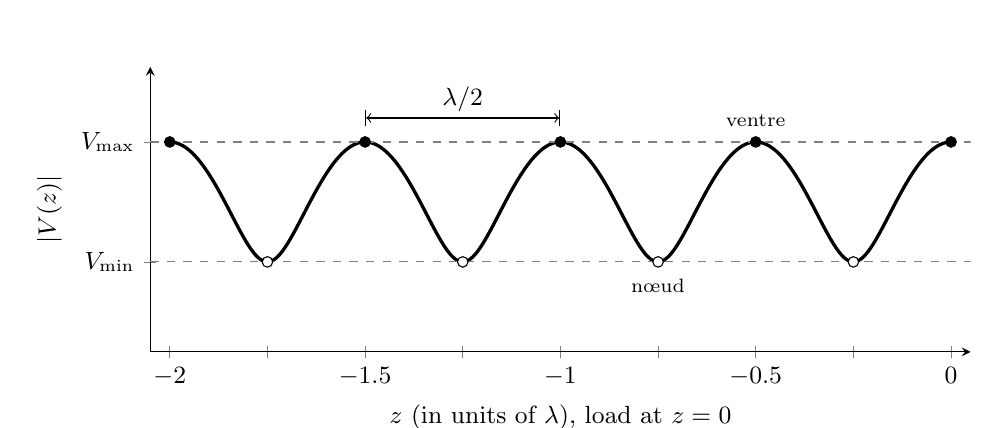
\begin{tikzpicture}
    \begin{axis}[
      width=12cm, height=5.2cm,
      xlabel={$z$ (in units of $\lambda$), load at $z=0$},
      ylabel={$|V(z)|$},
      xmin=-2.05, xmax=0.05, ymin=0, ymax=1.9,
      xtick={-2,-1.75,-1.5,-1.25,-1,-0.75,-0.5,-0.25,0},
      xticklabels={$-2$,,$-1.5$,,$-1$,,$-0.5$,,$0$},
      ytick={0.6,1.4}, yticklabels={$V_{\min}$,$V_{\max}$},
      grid=none, axis lines=left,
      tick label style={font=\small}, label style={font=\small},
      ]
      \addplot[very thick,domain=-2:0,samples=300]
        {sqrt(1.16 + 0.8*cos(720*x))};
      \addplot[only marks,mark=*,mark size=1.9pt]
        coordinates {(0,1.4) (-0.5,1.4) (-1,1.4) (-1.5,1.4) (-2,1.4)};
      \addplot[only marks,mark=*,mark size=1.9pt,fill=white]
        coordinates {(-0.25,0.6) (-0.75,0.6) (-1.25,0.6) (-1.75,0.6)};
      \draw[dashed,gray] (axis cs:-2.05,1.4) -- (axis cs:0.05,1.4);
      \draw[dashed,gray] (axis cs:-2.05,0.6) -- (axis cs:0.05,0.6);
      \draw[|<->|] (axis cs:-1.5,1.56) -- node[above,font=\small,inner sep=2pt]
        {$\lambda/2$} (axis cs:-1,1.56);
      \node[font=\scriptsize,anchor=north] at (axis cs:-0.75,0.55)
        {nœud};
      \node[font=\scriptsize,anchor=south] at (axis cs:-0.5,1.44)
        {ventre};
    \end{axis}
  \end{tikzpicture}
  \caption*{\small Enveloppe de la tension $V^{+}(z)+V^{-}(z)$ le long de la
  ligne de propagation, here for $|\Gamma| = 0{,}4$, so $V_{\max} = 1{,}4$,
  $V_{\min} = 0{,}6$ and $\mathrm{ROS} = 2{,}33$. Nœuds (open) and ventres
  (filled) are fixed in space and spaced by $\lambda/2$.}
\end{figure}

En un ventre, les tensions incidente et réfléchie sont \emph{en phase}, et
l'on a $V_{\max} = |V^{+}| + |V^{-}|$ ; en un nœud, elles sont en opposition de
phase, et l'on a $V_{\min} = |V^{+}| - |V^{-}|$.

\begin{definition}[Rapport d'onde stationnaire (ROS)]
  On caractérise ce phénomène de propagation par le \textbf{rapport d'onde
  stationnaire} (\textit{standing wave ratio}, ROS), VSWR (\textit{Voltage
  Standing Wave Ratio}) en anglais, défini par
  \[
    \mathrm{ROS} = \frac{V_{\max}}{V_{\min}}
                 = \frac{|V^{+}| + |V^{-}|}{|V^{+}| - |V^{-}|} .
  \]
\end{definition}

\begin{theorem}[ROS et $\Gamma$]
  On rencontre un phénomène de propagation par ondes stationnaires lorsque sur
  l'axe de propagation il existe une impédance de charge $Z_L$ différente de
  l'impédance caractéristique $Z_C$ de la ligne. Pour une ligne sans pertes,
  avec le module du facteur de réflexion
  $|\Gamma(z=0)| = |V_0^{-}|/|V_0^{+}| = \left|(Z_L-Z_C)/(Z_L+Z_C)\right|$,
  on peut écrire le ROS ainsi :
  \[
    \boxed{\;
    |\Gamma(z=0)| = \frac{\mathrm{ROS} - 1}{\mathrm{ROS} + 1},
    \qquad
    \mathrm{ROS} = \frac{1 + |\Gamma(z=0)|}{1 - |\Gamma(z=0)|} .
    \;}
  \]
\end{theorem}

À noter que $0 \le |\Gamma(z=0)| \le 1$ et naturellement
$1 \le \mathrm{ROS} < \infty$. Lorsque $\mathrm{ROS} \approx 1$, les impédances
$Z_L$ et $Z_C$ sont identiques : l'impédance de charge est alors adaptée à
l'impédance caractéristique de la ligne, et le maximum de puissance est transmis
et dissipé dans l'impédance de charge. Adaptation : $\mathrm{ROS} = 1$.

\subsubsection{Conséquences sur la puissance délivrée à l'impédance de charge}
Si un générateur RF fournit un signal de puissance de 1~mW à l'entrée d'une
ligne d'impédance caractéristique $Z_C = 50\ \Omega$, la puissance mesurée par
un wattmètre à la sortie, qui simule une impédance de charge, sera de 1~mW car
l'impédance d'entrée du wattmètre est aussi de $50\ \Omega$ : il y a alors
adaptation d'impédance entre l'impédance d'entrée du wattmètre et l'impédance
caractéristique du câble. Si maintenant on remplace la ligne par une ligne
d'impédance caractéristique $Z_C \ne 50\ \Omega$, la puissance mesurée par le
wattmètre sera inférieure à 1~mW, et d'autant plus inférieure que $Z_C$
s'éloigne de la valeur optimale de $50\ \Omega$ : il y a dans ce cas une
\emph{désadaptation d'impédance}.

\begin{example}[1~mW into a $50\ \Omega$ wattmètre through a lossless cable]
  \begin{center}
    \begin{tabular}{cc}
      \toprule
      $Z_C$ du câble & puissance mesurée par le wattmètre \\
      \midrule
      $10\ \Omega$  & $0{,}56$~mW \\
      $20\ \Omega$  & $0{,}82$~mW \\
      $\mathbf{50\ \Omega}$  & $\mathbf{1}$~\textbf{mW} \\
      $100\ \Omega$ & $0{,}89$~mW \\
      \bottomrule
    \end{tabular}
  \end{center}
  The full 1~mW arrives only for $Z_C = 50\ \Omega$.
\end{example}

\begin{remark}
  The rows are what $P = P_{inc}\left(1-|\Gamma_0|^2\right)$ with
  $\Gamma_0 = (50-Z_C)/(50+Z_C)$ predicts, to the digits shown: for the
  $20\ \Omega$ row, for instance, $|\Gamma_0| = 30/70$ gives
  $P = 0{,}82$~mW. The formula is the thing to reproduce.
\end{remark}

Pour une ligne avec pertes (réelle), il faudra ajouter l'atténuation $\alpha$
(on top of this désadaptation loss), mais ça ne sera pas étudié dans ce cours.

\subsection{Puissance transportée dans une ligne sans pertes}
Soit une ligne sans pertes, $\gamma = j\beta$, d'impédance caractéristique
$Z_C$, fermée sur une impédance de charge $Z_L$ quelconque et alimentée par un
générateur RF fournissant un signal $V_g(t)$ sinusoïdal. La tension et le
courant le long de cette ligne s'écrivent :
\[
  V(z) = V^{+}e^{-\gamma z} + V^{-}e^{+\gamma z},
  \qquad
  I(z) = \frac{1}{Z_C}\left(V^{+}e^{-\gamma z} - V^{-}e^{+\gamma z}\right).
\]
La puissance moyenne relevée à l'abscisse $z$ sur la ligne s'écrit :
\[
  P(z) = \Re\!\left[\tfrac{1}{2}\,V(z)\,I^{*}(z)\right].
\]

\begin{proof}
  Avec $\Gamma(z) = \dfrac{V_0^{-}}{V_0^{+}}e^{2j\beta z}$, on peut écrire
  (the voltage and current factorise)
  \[
    V(z) = V^{+}e^{-\gamma z}\left(1 + \Gamma(z)\right),
    \qquad
    I(z) = \frac{1}{Z_C}V^{+}e^{-\gamma z}\left(1 - \Gamma(z)\right),
  \]
  On obtient alors la puissance moyenne :
  \[
    P(z) = \frac{|V^{+}|^{2}}{2Z_C}\,
      \Re\!\left[e^{-(\gamma+\gamma^{*})z}
      \left(1+\Gamma(z)\right)\left(1-\Gamma^{*}(z)\right)\right].
  \]
  La ligne est sans pertes, $\gamma + \gamma^{*} = 0$ --- the exponential
  disappears --- alors :
  \[
    P(z) = \frac{|V^{+}|^{2}}{2Z_C}\,
      \Re\!\left[1 + \Gamma(z) - \Gamma^{*}(z) - \Gamma(z)\Gamma^{*}(z)\right].
  \]
  The middle two terms are purely imaginary and cancel under $\Re$ ; ce qui
  donne :
  \[
    P(z) = \frac{|V^{+}|^{2}}{2Z_C}\left[1 - |\Gamma(z)|^{2}\right]. \qed
  \]
\end{proof}

Le terme $\dfrac{|V^{+}|^{2}}{2Z_C}$ est donc la puissance moyenne transportée
par l'onde incidente. Dans le cas général d'une ligne sans pertes, sur laquelle
se propagent une onde incidente et une onde réfléchie, la puissance consommée
par l'impédance de charge dépend du seul module du facteur de réflexion
$|\Gamma(z=0)|$ :
\[
  P(z=0) = P_{inc}(z=0) - P_{ref}(z=0),
  \qquad
  P_{inc}(z=0) = \frac{|V_0^{+}|^{2}}{2Z_C},
  \qquad
  P_{ref}(z=0) = |\Gamma(z)|^{2}\,\frac{|V_0^{+}|^{2}}{2Z_C}.
\]
Si la ligne est sans pertes, la puissance incidente correspond à la puissance
délivrée par le générateur RF, et $|\Gamma(z)| = |\Gamma(z=0)| \equiv
|\Gamma_0|$ ne dépend pas de $z$.

\begin{theorem}[Bilan de puissance]
  Pour une ligne sans pertes d'impédance caractéristique $Z_C$ fermée sur une
  impédance de charge $Z_L$, la puissance moyenne réfléchie par la charge et la
  puissance moyenne absorbée par la charge s'écrivent
  \[
    \boxed{\;
    P_{ref} = |\Gamma_0|^{2}\,P_{inc},
    \qquad
    P = P_{inc}\left[1 - |\Gamma_0|^{2}\right],
    \qquad
    \Gamma_0 = \frac{Z_L - Z_C}{Z_L + Z_C},
    \;}
  \]
  avec $P_{inc}$ la puissance moyenne fournie par le générateur.
\end{theorem}

\begin{conclusion}
  A désadaptation costs power twice over: the fraction $|\Gamma_0|^2$ of the
  incident power never reaches the load at all, and the onde réfléchie that
  carries it back up the line disturbs the line and the functioning of the
  system feeding it. This is why the next chapter is about adaptation
  d'impédance.
\end{conclusion}

\subsection{Quelques références de valeur de puissance}
La puissance est exprimée en watts (W). Dans le domaine des systèmes RF et
hyperfréquences, on exprimera plus naturellement la puissance dans l'échelle
logarithmique, soit en dBm, soit en dBW.

\begin{definition}[dBm et dBW]
  \[
    P_{\mathrm{dBm}} = 10\log_{10}\left(P_{\mathrm{mW}}\right),
    \qquad
    P_{\mathrm{dBW}} = 10\log_{10}\left(P_{\mathrm{W}}\right),
  \]
  où $P_{\mathrm{mW}}$ est la puissance exprimée en milliwatts et
  $P_{\mathrm{W}}$ la puissance exprimée en watts. On utilise le dBm pour les
  communications sans fil terrestres à courtes et moyennes distances ($<2$ ou
  3~km), entraînant des puissances maximales de l'ordre du watt ; on utilise le
  dBW pour les communications par satellites ou les radars, pour des distances
  $>10$~km où de fortes puissances sont utilisées, de l'ordre de plusieurs
  dizaines de watts à centaines de kilowatts.
\end{definition}

\begin{center}
  \begin{tabular}{ccc}
    \toprule
    Puissance en W & Puissance en dBm & Puissance en dBW \\
    \midrule
    $0{,}1$~mW & $-10$~dBm & $-40$~dBW \\
    $1$~mW     & $0$~dBm   & $-30$~dBW \\
    $10$~mW    & $10$~dBm  & $-20$~dBW \\
    $20$~mW    & $13$~dBm  & $-17$~dBW \\
    $100$~mW   & $20$~dBm  & $-10$~dBW \\
    $1$~W      & $30$~dBm  & $0$~dBW \\
    \bottomrule
  \end{tabular}
\end{center}

On peut ainsi extrapoler facilement à plusieurs centaines de watts, et on
remarque aussi que
\[
  \boxed{\; P_{\mathrm{dBm}} = P_{\mathrm{dBW}} + 30\ \mathrm{dB}. \;}
\]

\begin{example}[Orders of magnitude for WiFi]
  À l'émission, la puissance maximale ne peut dépasser (norme standardisée)
  100~mW, soit 20~dBm. En réception, les valeurs de puissance sont comprises
  entre $-30$ et $-90$~dBm. À $-30$~dBm, la puissance de réception est
  excellente ; entre $-50$ et $-60$~dBm, la qualité du réseau sans fil est
  qualifiée de correcte et la puissance est suffisante pour une activité
  « normale » sur internet ; à $-90$~dBm, la connexion est réellement mauvaise,
  et il est probable que l'on ne pourra pas se connecter.
\end{example}

\subsection{Étude de la ligne coaxiale}
The same results can be established from the fields rather than from a circuit
model --- une démonstration du passage de la notion champ électrique/champ
magnétique à la notion tension/courant se propageant le long d'une ligne
coaxiale --- and the intermediate results are worth keeping. Les conducteurs
sont constitués de métal parfait supposé sans pertes ; le diélectrique
intérieur est supposé linéaire et isotrope, avec pour paramètres constitutifs
$\varepsilon = \varepsilon' - j\varepsilon''$ et $\mu$.

\begin{example}[From Maxwell in cylindrical coordinates to the équations des télégraphistes]
  \textbf{Mode TEM et symétrie azimutale.} Pour un mode TEM, les 2 champs sont
  transverses, ce qui implique $E_z = H_z = 0$ ; la symétrie azimutale rend les
  champs invariants selon la coordonnée $\varphi$ : $\partial/\partial\varphi = 0$.
  L'équation de Maxwell--Ampère, en l'absence de courant de conduction,
  s'écrit $\curl \v{H} = j\omega\varepsilon\v{E}$, et l'équation de
  Maxwell--Faraday $\curl \v{E} = -j\omega\mu\v{H}$ ; le rotationnel d'un
  vecteur quelconque, en coordonnées cylindriques, s'écrit
  \[
    \curl \v{V} =
      \left[\frac{1}{\rho}\frac{\del V_z}{\del \varphi}
            - \frac{\del V_\varphi}{\del z}\right]\unitv{u}_\rho
    + \left[\frac{\del V_\rho}{\del z}
            - \frac{\del V_z}{\del \rho}\right]\unitv{u}_\varphi
    + \frac{1}{\rho}\left[\frac{\del (\rho V_\varphi)}{\del \rho}
            - \frac{\del V_\rho}{\del \varphi}\right]\unitv{u}_z
  \]
  et, en projetant sur $\unitv{u}_z$, on obtient
  $\frac{1}{\rho}\frac{\del(\rho H_\varphi)}{\del\rho} = j\omega\varepsilon E_z = 0$
  et
  $\frac{1}{\rho}\frac{\del(\rho E_\varphi)}{\del\rho} = -j\omega\mu H_z = 0$,
  d'où
  \[
    \rho H_\varphi = g(z), \qquad \rho E_\varphi = f(z),
    \qquad \text{and, on } \unitv{u}_\rho, \quad \rho E_\rho = h(z).
  \]

  \textbf{Conditions de continuité des champs.} Le champ tangentiel est nul sur les parois
  du métal supposé parfait en $\rho = a$ et $\rho = b$ pour tout $z$, d'où
  $E_\varphi = f(z)/a = f(z)/b = 0$, donc $E_\varphi = 0$ et, d'après
  $\del E_\varphi/\del z = j\omega\mu H_\rho$, $H_\rho = 0$. What survives is a
  radial $\v{E}$ and an azimuthal $\v{H}$; finalement les équations de Maxwell
  s'écrivent :
  \[
    \frac{\del h(z)}{\del z} = -j\omega\mu\, g(z),
    \qquad
    \frac{\del g(z)}{\del z} = -j\omega\varepsilon\, h(z).
  \]

  \textbf{Équivalence de la description en champs avec la description en
  courant tension $V$ et $I$.} Dans le plan transverse, le potentiel
  vecteur n'a pas de composante transverse, donc on aura alors
  $\v{E} = -\grad V$ simplement, et
  \[
    V(z) = \int_a^b E_\rho\, d\rho = h(z)\ln\!\left(\frac{b}{a}\right),
    \qquad
    I(z) = \oint \v{H}\cdot d\v{l} = \int_0^{2\pi} H_\varphi\,\rho\, d\varphi
         = 2\pi\, g(z),
  \]
  la seconde en calculant la circulation sur un cercle de rayon $a$ (théorème
  d'Ampère). En injectant ces expressions dans les équations couplées, on
  obtient les équations des télégraphistes
  \[
    dV(z) = -j\omega L\, I(z)\, dz,
    \qquad
    dI(z) = -(G + j\omega C)\, V(z)\, dz,
  \]
  with exactly the éléments distribués the circuit model postulates:
  \[
    L = \frac{\mu\ln(b/a)}{2\pi},
    \qquad
    C = \frac{2\pi\varepsilon'}{\ln(b/a)},
    \qquad
    G = \frac{2\pi\omega\varepsilon''}{\ln(b/a)} .
  \]
\end{example}

\begin{remark}[What the derivation adds]
  Three things beyond the circuit model. First, $G$, qui représente les pertes
  diélectriques, is tied to the imaginary part $\varepsilon''$ of the
  permittivité, so ``pertes diélectriques'' and
  $\tan\delta = \varepsilon''/\varepsilon'$ are the same statement. Second, in
  the lossless case ($G=0$) the constante de propagation
  $\gamma = 0 + j\omega\sqrt{LC}$ obtained on the line est \emph{la même} que
  celle qui serait obtenue dans le diélectrique illimité --- the line does not
  change the physics of the medium, it only channels it. Third, the physical
  model is not unique: many models en éléments localisés reproduce the same
  equations, and dans le cas d'un métal à pertes, une résistance série
  viendrait s'ajouter avec l'inductance $L$.
\end{remark}

\begin{prop}[Vitesse de phase et longueur d'onde dans la ligne]
  \[
    v_\varphi = \frac{\omega}{\beta} = \frac{1}{\sqrt{\varepsilon\mu}},
    \qquad
    \lambda = v_\varphi T = \frac{2\pi}{\beta},
  \]
  valeurs qui sont aussi celles qui seraient obtenues dans le diélectrique
  illimité. L'impédance caractéristique s'obtient en dérivant les solutions
  générales et en identifiant :
  $Z_C = V_0^{+}/I_0^{+} = -V_0^{-}/I_0^{-} = \sqrt{L/C}$.
\end{prop}

\begin{remark}
  Quand il n'y a pas d'ondes réfléchies, $V_0^{-} = I_0^{-} = 0$, et dans ce
  cas l'impédance vue le long de la ligne est constante quel que soit $z$, et
  elle est égale à l'impédance caractéristique $Z_C$. This is the operational
  content of the ``physical meaning of $Z_C$'' remark: $Z_C$ is what an
  infinitely long line --- or one closed on a charge adaptée --- presents.
\end{remark}

\begin{remark}[Why $\Gamma$ and not $V$ is what gets measured]
  Il est extrêmement difficile et coûteux (voire impossible pour des fréquences
  supérieures à 100~GHz) de mesurer la tension pour des fréquences élevées. Le
  facteur de réflexion permet, dans la pratique, de caractériser des
  dispositifs sous test : sa mesure est basée sur la mesure de la puissance
  réfléchie à l'interface d'un dispositif (ou charge) et de la ligne de
  propagation amenant le signal. Cette méthode est réalisable, à relativement
  bas coût, jusqu'à des fréquences extrêmement élevées (quelques THz) --- which
  is why $\Gamma$, and the paramètres S built from it in the next chapter, is
  the currency of RF characterisation.
\end{remark}

\section{Adaptation d'impédance dans les lignes de transmission --- introduction aux paramètres S}
A ligne sans pertes of impédance caractéristique $Z_C$ closed on a load $Z_L \neq Z_C$
reflects part of the incident power back towards the generator. L'objectif de
l'adaptation d'impédance est de transmettre le maximum de puissance du générateur
vers le récepteur ou l'impédance de charge $Z_L$. It is done by inserting a lossless
reactive network between the line and the load.
The second half of the chapter answers the measurement question that follows: above
a gigahertz the voltages and currents a $Z$ matrix is built from cannot be measured,
so a multipôle is characterised instead by the matrice S, whose entries relate the
ondes de puissance entering the device to the ondes de puissance leaving it.

\begin{notation}
  $Z_C$ is the impédance caractéristique of the line, $Z_G$ the internal impedance of
  the generator, $Z_L$ the load, $Z_E$ the equivalent impedance seen looking into the
  matching network plus the load, and $Z_0$ the impédance de référence of the
  paramètres S. $\beta = 2\pi/\lambda$ is the constante de phase, $\Gamma$ the facteur
  de réflexion, $Y = 1/Z$ an admittance. Unless said otherwise every line in this
  chapter is a ligne sans pertes, so $\beta$ is real and $Z_C$ is real; in practice
  $Z_C = Z_0 = 50\ \Omega$.
\end{notation}

\subsection{Adaptation d'impédances dans les lignes de transmission : introduction}
L'impédance de charge $Z_L$ modélise l'accès du composant ou de la fonction
(amplificateurs, filtres, antennes\dots) suivante intervenant dans une chaîne de
transmission ou une chaîne de réception d'un système de communication. Il est d'autant
plus important d'optimiser et de maximiser ce transfert de puissance utile notamment
pour des systèmes autonomes (smartphones, tablettes, IoT\dots) afin de préserver les
batteries par exemple. Il est donc indispensable d'éviter toutes pertes de puissance
par réflexion due à une désadaptation d'impédance.

Le problème se pose et se résout à deux niveaux : au niveau du générateur et au niveau
de l'impédance de charge. Il faut que, d'une part, le générateur puisse transmettre à
la ligne le maximum de puissance (puissance disponible) et, d'autre part, que le
récepteur reçoive de la ligne le plus possible de cette puissance. \textbf{Dans ce
cours on supposera que le générateur présente une impédance interne adaptée à
l'impédance caractéristique des lignes utilisées}, $Z_G = Z_C$. Only the load end is
therefore ever worked on.

\begin{remark}
  Reflection is not only a loss of efficiency. Lorsqu'une onde est réfléchie, un
  régime d'onde stationnaire existe dans la ligne. La conséquence peut être dans le
  meilleur des cas un système fonctionnant mal et, dans le pire cas, la destruction de
  certains composants du système. It is the voltage maxima of the standing wave that
  destroy them.
\end{remark}

The matching device is a lossless quadripôle, written $Q_{\text{match}}$, inserted
between the line and the load. Un observateur situé à gauche du quadripôle
d'adaptation doit voir une impédance équivalente du système --- quadripôle +
impédance de charge --- égale à l'impédance caractéristique de la ligne, et donc
obtenir un facteur de réflexion, du système quadripôle + impédance de charge, nul.

\begin{figure}[h!]
  \centering
  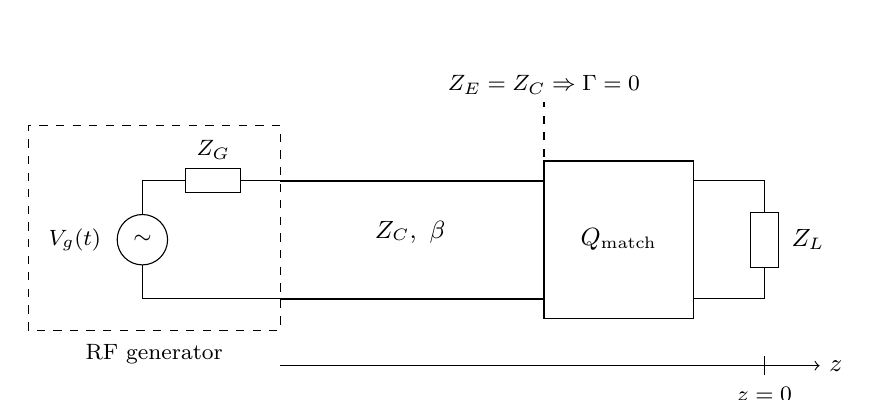
\begin{tikzpicture}[every node/.style={font=\small}]
    % generator
    \draw[dashed] (-1.45,-1.15) rectangle (1.75,1.45);
    \node[font=\footnotesize] at (0.15,-1.45) {RF generator};
    \draw (0,-0.32) -- (0,-0.75) -- (1.75,-0.75);
    \draw (0,0.32) -- (0,0.75) -- (0.55,0.75);
    \draw (0,0) circle (0.32);
    \node[font=\footnotesize] at (0,0) {$\sim$};
    \node[left,font=\footnotesize] at (-0.4,0) {$V_g(t)$};
    \draw (0.55,0.6) rectangle (1.25,0.9);
    \node[above,font=\footnotesize] at (0.9,0.9) {$Z_G$};
    \draw (1.25,0.75) -- (1.75,0.75);
    % line
    \draw[thick] (1.75,0.75) -- (5.1,0.75);
    \draw[thick] (1.75,-0.75) -- (5.1,-0.75);
    \node at (3.4,0.1) {$Z_C,\ \beta$};
    % matching network
    \draw (5.1,-1.0) rectangle (7.0,1.0);
    \node at (6.05,0) {$Q_{\text{match}}$};
    % load
    \draw (7.0,0.75) -- (7.9,0.75) -- (7.9,0.35);
    \draw (7.72,-0.35) rectangle (8.08,0.35);
    \node[right] at (8.12,0) {$Z_L$};
    \draw (7.9,-0.35) -- (7.9,-0.75) -- (7.0,-0.75);
    % axis and reference plane
    \draw[->] (1.75,-1.6) -- (8.6,-1.6) node[right] {$z$};
    \draw (7.9,-1.72) -- (7.9,-1.48);
    \node[below,font=\footnotesize] at (7.9,-1.75) {$z=0$};
    \draw[dashed] (5.1,1.05) -- (5.1,1.75);
    \node[above,font=\footnotesize] at (5.1,1.72) {$Z_E = Z_C \Rightarrow \Gamma = 0$};
  \end{tikzpicture}
  \caption*{Principe de l'adaptation d'impédance. The lossless network
  $Q_{\text{match}}$ turns $Z_L$ into $Z_C$ at its input plane, so nothing is reflected
  back down the line.}
\end{figure}

\begin{prop}[Condition d'adaptation (\textit{matching condition})]
  Written at the generator, the condition reads: adaptation si
  \[Z_C = Z_E^{*},\]
  $Z_E$ étant l'impédance équivalente à $Z_L$ + $Q_{\text{match}}$. Pour une
  ligne sans pertes $Z_C \in \reals$; the condition then reduces to
  \[\boxed{\,Z_E = Z_C\,}\]
  which is the form used everywhere below.
\end{prop}

Afin de limiter les pertes de puissance, il faut de plus que le quadripôle
d'adaptation soit sans pertes afin de ne pas perdre inutilement de la puissance utile.
Pour réaliser cette adaptation d'impédance, on ajoutera des éléments réactifs en série
ou en parallèle, ces éléments étant soit des éléments dits localisés (capacités,
inductances), soit des tronçons de lignes sans pertes. Éléments localisés : composants
réels mais qualité moindre avec les pertes; they are, however, easy to place.
Éléments distribués : réaliser les inductances et capacités avec des tronçons de lignes
(pas de --- ou moins de --- pertes, mais taille !).

\begin{remark}
  En électronique basse fréquence, on utilise aussi le terme d'adaptation
  d'impédance. Un oscilloscope ou un amplificateur, par exemple, possèdent une
  impédance d'entrée très grande pour éviter de diminuer la tension que l'oscilloscope
  doit mesurer ou que l'amplificateur doit amplifier. La source de tension au contraire
  doit posséder une impédance de sortie la plus faible possible. Contrairement à notre
  préoccupation, il ne s'agit pas là d'optimiser le transfert de puissance mais de
  s'arranger pour ne pas écraser la tension disponible.
\end{remark}

\begin{remark}[Warning]
  On ne peut pas adapter une impédance $Z_L$ purement réactive : il faut
  obligatoirement que $Z_L$ possède une partie résistive pour absorber la puissance
  incidente.
\end{remark}

Les dispositifs d'adaptation, que l'on va analyser, sont des dispositifs \textbf{à
bande passante étroite} (\textit{narrowband}) :
\begin{subpart}
  \item l'adaptation en série par une ligne quart d'onde ($\lambda/4$) ou
    transformateur d'impédance ;
  \item l'adaptation en parallèle par l'ajout d'une ligne sans pertes appelée
    \textit{stub} ;
  \item l'adaptation par éléments localisés (quadripôle en « L »).
\end{subpart}

\subsection{Adaptation d'impédance par une ligne quart d'onde ou transformateur d'impédance}
The starting point is the \textit{impédance ramenée} --- the impedance a load presents
after being carried back along a length of line --- established for a ligne sans pertes
as
\[Z(z = -l) = Z_C\,\frac{Z_L + j Z_C \tan(\beta l)}{Z_C + j Z_L \tan(\beta l)}.\]

\begin{prop}[Transformateur d'impédance]
  For $l = \lambda/4$ one has $\beta l = \pi/2$ and $\tan(\beta l) \to \infty$. On
  montre alors que l'impédance
  \[\boxed{\;Z_E = Z\!\left(z = -\lambda/4\right) = \frac{Z'^{\,2}_C}{Z_L}\;}\]
  avec $Z_L$ l'impédance de charge vue sur l'accès opposé de la ligne d'impédance
  caractéristique $Z'_C$, réelle et quelconque. The ligne quart d'onde inverts the load
  about $Z'_C$; this is what makes it a transformateur d'impédance.
\end{prop}

\begin{figure}[h!]
  \centering
  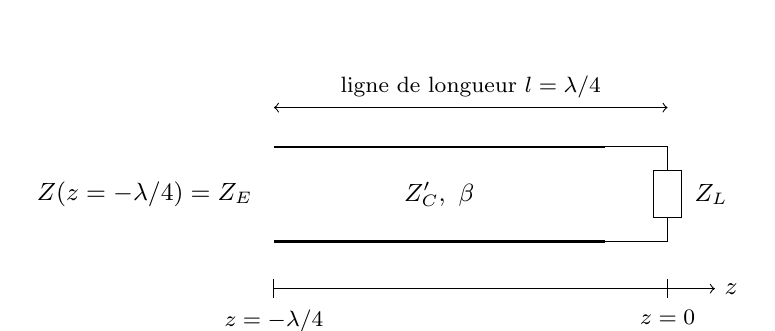
\begin{tikzpicture}[every node/.style={font=\small}]
    \draw[thick] (0,0.6) -- (4.2,0.6);
    \draw[thick] (0,-0.6) -- (4.2,-0.6);
    \node at (2.1,0) {$Z'_C,\ \beta$};
    \draw (4.2,0.6) -- (5.0,0.6) -- (5.0,0.3);
    \draw (4.82,-0.3) rectangle (5.18,0.3);
    \node[right] at (5.22,0) {$Z_L$};
    \draw (5.0,-0.3) -- (5.0,-0.6) -- (4.2,-0.6);
    \draw[<->] (0,1.1) -- (5.0,1.1);
    \node[above,font=\footnotesize] at (2.5,1.1) {ligne de longueur $l = \lambda/4$};
    \draw[->] (0,-1.2) -- (5.6,-1.2) node[right] {$z$};
    \draw (0,-1.32) -- (0,-1.08);
    \draw (5.0,-1.32) -- (5.0,-1.08);
    \node[below,font=\footnotesize] at (0,-1.35) {$z = -\lambda/4$};
    \node[below,font=\footnotesize] at (5.0,-1.35) {$z = 0$};
    \node[left] at (-0.15,0) {$Z(z=-\lambda/4) = Z_E$};
  \end{tikzpicture}
  \caption*{\textit{Impédance ramenée} sur une longueur $l = \lambda/4$.}
\end{figure}

\paragraph{Cas d'une impédance de charge réelle.} On cherche ici à obtenir
$Z_E = Z_C$ où $Z_C$ est l'impédance de référence (exclusivement $50\ \Omega$ dans ce
cours). Setting $Z'^{\,2}_C/Z_L = Z_C$ gives the result to remember: l'adaptation sera
réalisée en utilisant une ligne de longueur $\lambda/4$ d'impédance caractéristique
\[\boxed{\;Z'_C = \sqrt{Z_L Z_C}\;}\]

\begin{remark}[Warning]
  $\lambda$ est la longueur d'onde \emph{dans le matériau} --- tenir compte de la
  permittivité relative $\varepsilon_r$. So $\lambda = c/(f\sqrt{\varepsilon_r})$ and
  the physical length is $l = \lambda/4 = c/(4 f \sqrt{\varepsilon_r})$.
\end{remark}

\paragraph{Cas d'une impédance de charge complexe.} L'impédance caractéristique des
lignes utilisées est réelle afin de ne pas avoir de pertes durant la propagation; a
transformateur d'impédance built from such a line can only invert a real quantity.
Dans ce cas, pour utiliser un transformateur d'impédance, il faut absolument éliminer
la partie imaginaire de l'impédance de charge dans un premier temps :
\begin{subpart}
  \item soit en ajoutant une impédance purement imaginaire (ici $-jX$) pour compenser
    la partie imaginaire --- for a load $Z_L = R + jX$ this leaves $R$ ;
  \item soit en ajoutant un tronçon de ligne d'impédance caractéristique $Z_C$ et de
    longueur $l'$ à ajuster en fonction de la partie imaginaire $jX$ à éliminer ---
    again leaving a real $Z_L = R$ at the plane where the transformateur d'impédance
    starts.
\end{subpart}
Dans les 2 cas, on peut ajouter ensuite la ligne d'impédance caractéristique $Z'_C$ de
longueur $\lambda/4$ pour réaliser l'adaptation finale.

\subsection{Adaptation d'impédance par l'ajout d'un STUB}
\begin{definition}[Stub]
  Un \textit{stub} est un tronçon de ligne sans pertes, associé en parallèle à la ligne
  principale, et terminé par une impédance purement réactive, c'est-à-dire un circuit
  ouvert (CO) ou un court-circuit (CC). Hypothèses : $\beta$ et impédance
  caractéristique identiques à celles de la ligne principale.
\end{definition}

The stub is tapped at the abscissa $z = -d$ and has its own length $d'$. L'adaptation
est obtenue en calculant les longueurs $d$ et $d'$, différentes si on choisit un stub
CC ou un stub CO.

\begin{figure}[h!]
  \centering
  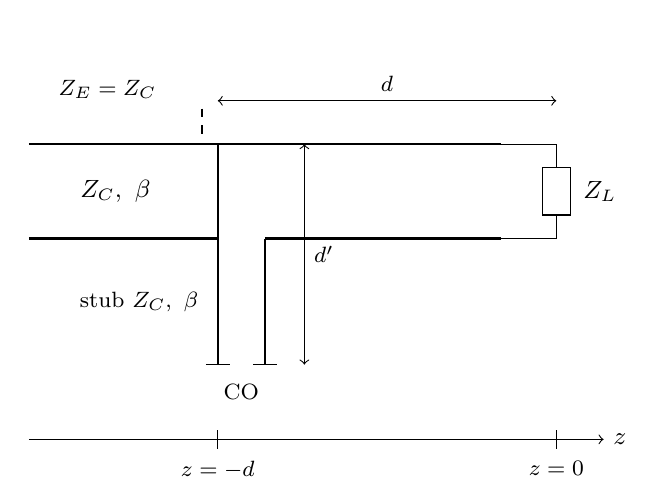
\begin{tikzpicture}[every node/.style={font=\small}]
    % main line
    \draw[thick] (0,0.6) -- (6.0,0.6);
    \draw[thick] (0,-0.6) -- (2.4,-0.6);
    \draw[thick] (3.0,-0.6) -- (6.0,-0.6);
    \node at (1.1,0) {$Z_C,\ \beta$};
    % load
    \draw (6.0,0.6) -- (6.7,0.6) -- (6.7,0.3);
    \draw (6.52,-0.3) rectangle (6.88,0.3);
    \node[right] at (6.92,0) {$Z_L$};
    \draw (6.7,-0.3) -- (6.7,-0.6) -- (6.0,-0.6);
    % stub branch, open-circuited
    \draw[thick] (2.4,0.6) -- (2.4,-2.2);
    \draw[thick] (3.0,-0.6) -- (3.0,-2.2);
    \draw (2.25,-2.2) -- (2.55,-2.2);
    \draw (2.85,-2.2) -- (3.15,-2.2);
    \node[font=\footnotesize] at (2.7,-2.55) {CO};
    \node[font=\footnotesize] at (1.4,-1.4) {stub $Z_C,\ \beta$};
    \draw[<->] (3.5,0.6) -- (3.5,-2.2);
    \node[right,font=\footnotesize] at (3.5,-0.8) {$d'$};
    % distances
    \draw[<->] (2.4,1.15) -- (6.7,1.15);
    \node[above,font=\footnotesize] at (4.55,1.15) {$d$};
    \draw[->] (0,-3.15) -- (7.3,-3.15) node[right] {$z$};
    \draw (2.4,-3.27) -- (2.4,-3.03);
    \draw (6.7,-3.27) -- (6.7,-3.03);
    \node[below,font=\footnotesize] at (2.4,-3.3) {$z = -d$};
    \node[below,font=\footnotesize] at (6.7,-3.3) {$z = 0$};
    \draw[dashed] (2.2,1.05) -- (2.2,0.7);
    \node[above,font=\footnotesize] at (1.0,1.05) {$Z_E = Z_C$};
  \end{tikzpicture}
  \caption*{Conditions d'adaptation par un STUB (ici fermé sur un CO).}
\end{figure}

\begin{prop}[Conditions d'adaptation par un STUB]
  Les conditions d'adaptation sont obtenues lorsque l'impédance globale $Z_E$, formée
  par l'association en \emph{parallèle} de l'impédance $Z_L$ ramenée d'une distance
  $d$ et du stub de longueur $d'$, vérifie $Z_E = Z_C$. Puisque le stub et l'impédance
  de charge ramenée sont en parallèle, on va raisonner en admittance :
  \[\boxed{\;Y_E = Y_C\;}\qquad Y_E = \frac{1}{Z_E},\quad Y_C = \frac{1}{Z_C},\]
  avec
  \[Y_E = \frac{1}{Z_E} = Y_{\text{STUB}} + Y_{Z_L}(z = -d), \qquad
    Y_{Z_L}(z = -d) = \frac{1}{Z(z=-d)}
      = Y_C\,\frac{Z_C + j Z_L \tan(\beta d)}{Z_L + j Z_C \tan(\beta d)}.\]
\end{prop}

En fonction de la terminaison du STUB, on détermine son admittance à partir de
l'expression de l'\textit{impédance ramenée} à l'abscisse $z = -d'$ :
\[
  \text{CO:}\quad Z_{CO} = \infty,\quad
  Y_{\text{STUB}}(z=-d') = \frac{j\tan(\beta d')}{Z_C};
  \qquad
  \text{CC:}\quad Z_{CC} = 0,\quad
  Y_{\text{STUB}}(z=-d') = \frac{1}{j Z_C \tan(\beta d')}.
\]
Equivalently, the stub closed on a circuit ouvert carries back
$Z'_{\text{STUB}} = -jZ_C\cot(\beta d')$.

\begin{remark}
  Each of these three admittances is the reciprocal of the \textit{impédance ramenée}
  $Z(z=-l) = Z_C (Z_L + jZ_C\tan\beta l)/(Z_C + jZ_L\tan\beta l)$ taken over the
  relevant length with the relevant termination (the load, a circuit ouvert or a
  court-circuit), so the tangent's argument is a real electrical length:
  $\tan(\beta d)$ on the load branch, $\tan(\beta d')$ on the stub. The constante de
  phase being real, these tangents are real and contribute no imaginary part of their
  own: on the load branch, for instance, $\tan(\beta d)$ only scales the terms it
  multiplies, and any imaginary part comes from an explicit $j$ or from a complex load.
\end{remark}

\begin{remark}
  Les longueurs $d$ et $d'$ sont déterminées «~modulo~» $\lambda/2$. Il existe donc
  une infinité de solutions, ce qui laisse la possibilité d'éloigner plus ou moins le
  stub de l'impédance de charge. En pratique, on essaie de limiter les longueurs $d$ et
  $d'$ car les lignes ne sont pas parfaites. On peut ainsi jouer sur le choix d'un STUB
  CO ou STUB CC qui permettra de trouver le meilleur compromis. \textbf{Dans ce cours,
  on vous donnera directement la terminaison du STUB pour l'adaptation.}
\end{remark}

\begin{example}[Stub fermé par un circuit ouvert, impédances réelles]
  Les impédances mises en jeu sont réelles. Writing $t = \tan(\beta d)$ and
  rationalising,
  \[Y_{Z_L}(z=-d) = Y_C\,\frac{Z_C Z_L (1+t^2) + j\,t\,(Z_L^2 - Z_C^2)}{Z_L^2 + Z_C^2 t^2},
    \qquad Y_{\text{STUB}} = j Y_C \tan(\beta d').\]
  Setting $Y_E = Y_C$ splits into a real and an imaginary equation. The real part gives
  $Z_C Z_L(1+t^2) = Z_L^2 + Z_C^2 t^2$, i.e.\ $t^2 Z_C(Z_L - Z_C) = Z_L(Z_L - Z_C)$, hence
  \[\boxed{\;\tan(\beta d) = \sqrt{\frac{Z_L}{Z_C}}\;}\]
  Substituting $t^2 = Z_L/Z_C$ into the imaginary part,
  $\tan(\beta d') = -t(Z_L^2-Z_C^2)/(Z_L^2 + Z_C^2 t^2)$, and since
  $Z_L^2 + Z_C^2 t^2 = Z_L(Z_L + Z_C)$,
  \[\boxed{\;\tan(\beta d') = \frac{Z_C - Z_L}{\sqrt{Z_L Z_C}}\;}\]
  Note that $d$ depends only on the ratio $Z_L/Z_C$: the tapping point is the abscissa
  at which the real part of the carried-back admittance is already $Y_C$, and the stub
  then cancels what is left of the susceptance.
\end{example}

\subsection{Adaptation par éléments localisés : quadripôle en « L »}
L'adaptation par éléments localisés consiste à insérer, entre la ligne de propagation
et l'impédance de charge $Z_L$, un quadripôle en forme de « L » constitué de deux
impédances purement imaginaires et matérielles, représentées par $jX_S$ (en série) et
$jX_P$ (en parallèle). Elles sont purement imaginaires afin de ne pas dissiper de
puissance inutilement : l'adaptation se fait avec des impédances qui ne dissipent pas
de puissance afin d'en conserver l'intégralité pour la dissiper dans $Z_L$.

\begin{prop}[Choix de la structure]
  Il y a deux structures possibles. Le choix de la structure dépend de la valeur de la
  partie réelle de l'impédance $Z_L$ à adapter par rapport à $Z_C$ :
  \begin{subpart}
    \item si $Z_L > Z_C$, on mettra en parallèle l'impédance de charge $Z_L$ avec
      l'impédance $jX_P$, le tout sera en série avec $jX_S$, soit
      $Z_E = jX_S + (Z_L \parallel jX_P)$ ;
    \item si $Z_L < Z_C$, on mettra en série l'impédance de charge $Z_L$ avec
      l'impédance $jX_S$, le tout en parallèle avec $jX_P$, soit
      $Z_E = jX_P \parallel (Z_L + jX_S)$.
  \end{subpart}
  Dans les deux cas, l'adaptation est obtenue quand l'impédance globale formée par
  $Z_L$, $jX_S$ et $jX_P$ est égale à $Z_C$.
\end{prop}

\begin{figure}[h!]
  \centering
  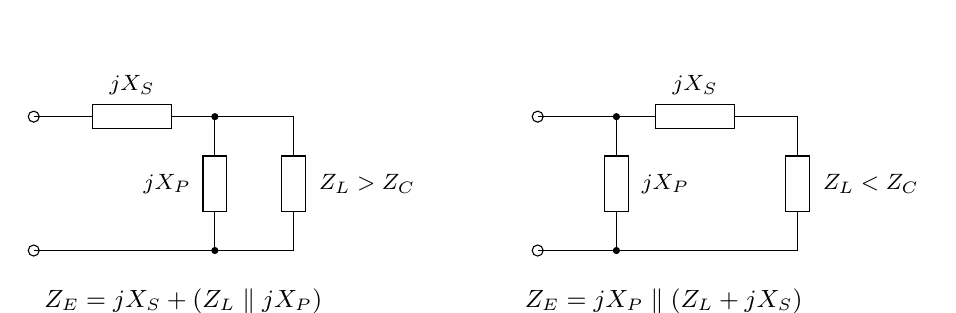
\begin{tikzpicture}[every node/.style={font=\small}]
    % LEFT : ZL > ZC
    \begin{scope}
      \draw (0,1.1) -- (0.75,1.1);
      \draw (0.75,0.95) rectangle (1.75,1.25);
      \node[above,font=\footnotesize] at (1.25,1.25) {$jX_S$};
      \draw (1.75,1.1) -- (3.3,1.1);
      \fill (2.3,1.1) circle (1.3pt);
      \draw (2.3,1.1) -- (2.3,0.6);
      \draw (2.15,-0.1) rectangle (2.45,0.6);
      \node[left,font=\footnotesize] at (2.12,0.25) {$jX_P$};
      \draw (2.3,-0.1) -- (2.3,-0.6);
      \draw (3.3,1.1) -- (3.3,0.6);
      \draw (3.15,-0.1) rectangle (3.45,0.6);
      \node[right,font=\footnotesize] at (3.5,0.25) {$Z_L > Z_C$};
      \draw (3.3,-0.1) -- (3.3,-0.6);
      \draw (0,-0.6) -- (3.3,-0.6);
      \fill (2.3,-0.6) circle (1.3pt);
      \draw (0,1.1) circle (0.07);
      \draw (0,-0.6) circle (0.07);
      \node at (1.9,-1.25) {$Z_E = jX_S + (Z_L \parallel jX_P)$};
    \end{scope}
    % RIGHT : ZL < ZC
    \begin{scope}[xshift=6.4cm]
      \draw (0,1.1) -- (1.5,1.1);
      \draw (1.5,0.95) rectangle (2.5,1.25);
      \node[above,font=\footnotesize] at (2.0,1.25) {$jX_S$};
      \draw (2.5,1.1) -- (3.3,1.1);
      \fill (1.0,1.1) circle (1.3pt);
      \draw (1.0,1.1) -- (1.0,0.6);
      \draw (0.85,-0.1) rectangle (1.15,0.6);
      \node[right,font=\footnotesize] at (1.2,0.25) {$jX_P$};
      \draw (1.0,-0.1) -- (1.0,-0.6);
      \draw (3.3,1.1) -- (3.3,0.6);
      \draw (3.15,-0.1) rectangle (3.45,0.6);
      \node[right,font=\footnotesize] at (3.5,0.25) {$Z_L < Z_C$};
      \draw (3.3,-0.1) -- (3.3,-0.6);
      \draw (0,-0.6) -- (3.3,-0.6);
      \fill (1.0,-0.6) circle (1.3pt);
      \draw (0,1.1) circle (0.07);
      \draw (0,-0.6) circle (0.07);
      \node at (1.6,-1.25) {$Z_E = jX_P \parallel (Z_L + jX_S)$};
    \end{scope}
  \end{tikzpicture}
  \caption*{The two ``L'' structures. Il y a 4 circuits possibles par structure suivant
  le choix des composants pour $jX_S$ et $jX_P$ (inductance-inductance,
  inductance-capacité, capacité-inductance et capacité-capacité). Le choix du type de
  composant se fait en fonction des valeurs réalisables.}
\end{figure}

\begin{example}[$Z_L = 200\ \Omega$ adapté to $Z_e = 50\ \Omega$ at $1\ \mathrm{GHz}$]
  Here $Z_L > Z_e$, so the first structure applies. Il faut débuter par
  $Z_e = jX_S + (Z_L \parallel jX_P)$ et développer la relation précédente. Taking
  $Z_L$ real, the development gives
  \[Z_e = \frac{Z_L X_P^2}{Z_L^2 + X_P^2}
        + j\left(X_S + \frac{Z_L^2 X_P}{Z_L^2 + X_P^2}\right).\]
  Ici $Z_e$ et $Z_L$ sont réelles, alors la partie imaginaire sera nulle. En séparant la
  partie réelle et imaginaire, on obtient alors 2 solutions possibles :
  \[X_P = \mp\, Z_L\sqrt{\frac{Z_e}{Z_L - Z_e}},
    \qquad X_S = \pm\sqrt{Z_e\,(Z_L - Z_e)}.\]
  Numerically, with $Z_L = 200\ \Omega$, $Z_e = 50\ \Omega$ and $F = 1\ \mathrm{GHz}$:
  \begin{center}
    \begin{tabular}{lrrll}
      \toprule
      & $X_P$ & $X_S$ & parallel branch & series branch \\
      \midrule
      Solution 1 & $-115\ \Omega$ & $+86\ \Omega$  & $C = 1.38$ pF & $L = 13.7$ nH \\
      Solution 2 & $+115\ \Omega$ & $-86\ \Omega$  & $L = 18$ nH   & $C = 1.85$ pF \\
      \bottomrule
    \end{tabular}
  \end{center}
  The identification of the component follows the sign of the reactance: une impédance
  imaginaire pure positive $jX = j L \omega$ est une inductance, donc $X = L\omega$ et
  $L = X/(2\pi F)$ ; une impédance imaginaire pure négative est une capacité, soit
  $jX = 1/(jC\omega) = -j/(C\omega)$ donc $X = -1/(C\omega)$ et
  $C = -1/(X\,2\pi F)$.
\end{example}

\begin{remark}
  Over a single denominator, the development above expresses the impédance d'entrée
  $Z_e$ in terms of the load $Z_L$ as
  $Z_e = \left(Z_L X_P^2 + j\left(Z_L^2(X_P + X_S) + X_P^2 X_S\right)\right)/(Z_L^2 + X_P^2)$.
  Since $Z_L$ and the target are both real, it is the bracket multiplying the imaginary
  unit in the numerator that must vanish.
\end{remark}

\begin{example}[$Z_L = 35\ \Omega$ adapté to $Z_e = 50\ \Omega$ at $1\ \mathrm{GHz}$]
  Now $Z_L < Z_e$, so the second structure applies. Il faut débuter par
  $Z_e = jX_P \parallel (Z_L + jX_S)$ ; en développant la relation précédente, on
  obtient
  \[Z_e = \frac{Z_L X_P^2}{Z_L^2 + (X_P + X_S)^2}
        + j\,\frac{X_P Z_L^2 + X_P X_S (X_P + X_S)}{Z_L^2 + (X_P + X_S)^2}.\]
  La partie imaginaire sera nulle ; on obtient alors 2 solutions possibles, with the
  roles of $Z_e$ and $Z_L$ exchanged relative to the previous case:
  \[X_P = \mp\, Z_e\sqrt{\frac{Z_L}{Z_e - Z_L}},
    \qquad X_S = \pm\sqrt{Z_L\,(Z_e - Z_L)}.\]
  \begin{center}
    \begin{tabular}{lrrll}
      \toprule
      & $X_P$ & $X_S$ & parallel branch & series branch \\
      \midrule
      Solution 1 & $-76\ \Omega$ & $+23\ \Omega$ & $C = 2.09$ pF  & $L = 3.66$ nH \\
      Solution 2 & $+76\ \Omega$ & $-23\ \Omega$ & $L = 12.1$ nH  & $C = 6.92$ pF \\
      \bottomrule
    \end{tabular}
  \end{center}
\end{example}

\begin{remark}
  The eight component values in the two tables follow from $L = X_S/(2\pi F)$ and
  $C = -1/(X_S\,2\pi F)$ at $F = 1\ \mathrm{GHz}$, and likewise for the parallel
  branch, applied to the rounded reactances of the tables. That rounding limits their
  precision: for the series inductance $L = 13.7$ nH of the first table,
  $X_S/(2\pi F)$ gives $13.69$ nH with the rounded $X_S = 86\ \Omega$, and $13.78$ nH
  with the unrounded $X_S = \sqrt{7500} = 86.6\ \Omega$.
\end{remark}

\begin{conclusion}
  The three devices answer the same equation $Z_E = Z_C$ with different hardware. The
  $\lambda/4$ transformateur d'impédance needs a real load and a line whose impédance
  caractéristique is a free design parameter; the stub needs only lines identical to
  the main one but two lengths to tune; the ``L'' network needs two reactive
  components and no line at all, at the cost of real components that have losses,
  where line sections have fewer losses but cost size. All three are à bande passante
  étroite, since each relies on a reactance or an electrical length that is correct at
  one frequency only.
\end{conclusion}

\subsection{Introduction aux paramètres S}
\subsubsection{La matrice Z en hyperfréquence}
Un \textbf{quadripôle} (\textit{two-port}) est un dispositif à 2 accès qui modélise le
transfert des grandeurs électriques, tension $V$ et courant $i$, au niveau de chaque
accès. Un \textbf{accès} (\textit{access}) est défini par 2 conducteurs simples séparés
par un diélectrique (par exemple une ligne de transmission) ; il est appelé
\textbf{dipôle} (\textit{one-port}). Un quadripôle est entièrement caractérisé par sa
matrice $Z$,
\[\begin{pmatrix} V_1 \\ V_2 \end{pmatrix}
  = Z \begin{pmatrix} i_1 \\ i_2 \end{pmatrix},
  \qquad
  \begin{cases} V_1 = Z_{11} i_1 + Z_{12} i_2 \\ V_2 = Z_{21} i_1 + Z_{22} i_2 \end{cases}\]
whose entries are obtained one at a time by opening one accès. For instance
\[Z_{11} = \left.\frac{V_1}{i_1}\right|_{i_2 = 0},\]
mesuré en fermant l'accès 2 sur un circuit ouvert ($i_2 = 0$), en connectant une
source de courant à l'accès 1 et en mesurant la tension $V_1$. For a T-shaped
resistive attenuator of arms $R_1, R_2, R_3$ this gives $Z_{11} = R_1 + R_2$,
$Z_{12} = Z_{21} = R_2$, $Z_{22} = R_2 + R_3$.

\begin{remark}[Measurement at hyperfréquences]
  Dans le cadre des fréquences très élevées (> GHz) : \textbf{hyperfréquences}
  (\textit{microwave}), microondes, mmW. There this procedure breaks down on three
  counts:
  \begin{subpart}
    \item les court-circuits et circuits ouverts sont difficiles à réaliser sur une
      large bande de fréquences, because the longueur d'onde becomes comparable with
      the dimensions of the lines and components, so the \textit{impédance ramenée} of
      a nominal short is not a short at the plane of interest;
    \item la mesure de la tension est complexe voire impossible (nécessite des ADCs
      ultra rapides) ;
    \item la réalisation des sources de courant est ardue.
  \end{subpart}
  La seule grandeur facilement mesurable en hyperfréquence est la \textbf{puissance}.
  La matrice $Z$ est très pratique mais très difficile à utiliser pour des fréquences
  très élevées.
\end{remark}

La \textbf{matrice S} (\textit{scattering matrix}) est un outil essentiel de
caractérisation de multipôles (dispositifs à $N$ accès) en hyperfréquence. Les facteurs de cette matrice, appelés \textbf{paramètres
S} (\textit{scattering parameter}), lient les puissances entrantes dans un multipôle
aux puissances sortantes, et sont basés uniquement sur des mesures de puissance. The
motivation is not academic: les puissances mises en jeu dans la majorité des
applications en hyperfréquence sont très faibles (pour la 5G, le seuil de détection
est fixé à une puissance de réception de $-102\ \mathrm{dBm}$, soit environ
$10^{-10}\ \mathrm{mW}$ ou $10^{-13}\ \mathrm{W}$). Connaître la distribution de la
puissance utile dans un dispositif est donc incontournable si on veut optimiser le
fonctionnement afin de limiter la consommation électrique et donc naturellement
prolonger l'autonomie des dispositifs sans fil.

\subsubsection{Notion d'onde de puissance}
Un multipôle linéaire à $N$ accès possède $2N$ pôles. On choisira une
\textbf{impédance de référence} (\textit{reference impedance}) des paramètres S,
réelle, que l'on notera $Z_0$. It is fixed once and for all. On note les tensions
incidentes $V_k^{+}$ et les courants incidents $I_k^{+}$ associés, dans le plan de
référence de l'accès $k$ ($k = 1 \dots N$), ainsi que les tensions réfléchies $V_k^{-}$
et les courants réfléchis $I_k^{-}$ associés. On écrit alors la tension totale et le
courant total à l'accès $k$ :
\[V_k = V_k^{+} + V_k^{-},
  \qquad I_k = I_k^{+} + I_k^{-} = \frac{1}{Z_0}\left(V_k^{+} - V_k^{-}\right),\]
equivalently $V_k^{+} = \tfrac{1}{2}(V_k + Z_0 I_k)$ and
$V_k^{-} = \tfrac{1}{2}(V_k - Z_0 I_k)$.

\begin{remark}
  The current relation is written here with the minus sign, as above: the incident and
  reflected currents are both counted along a single reference direction, towards the
  load, so the reflected current enters the total current with a minus sign. Another
  convention writes «~$V^{+} = Z_0 I^{+}$ et $V^{-} = Z_0 I^{-}$~», drawing
  $I^{-}$ as an arrow pointing back towards the source, i.e.\ $I^{-}$ taken as a
  magnitude along the reverse direction. The two conventions differ only in that
  reference direction for the reflected current: both give $\Gamma = V^{-}/V^{+}$ and
  the same power expressions below. These notes use the single reference direction
  throughout.
\end{remark}

La puissance des ondes incidentes ($P_k^{+}$) et réfléchies ($P_k^{-}$) sur l'accès $k$
s'exprime comme
\[P_k^{+} = \frac{1}{2}\Re\!\left(V_k^{+} I_k^{+*}\right)
          = \frac{1}{2}\Re\!\left(\frac{V_k^{+} V_k^{+*}}{Z_0}\right)
          = \frac{\left|V_k^{+}\right|^2}{2 Z_0},
  \qquad
  P_k^{-} = \frac{\left|V_k^{-}\right|^2}{2 Z_0}.\]
On pourrait caractériser le multipôle en reliant les puissances $P_k^{+}$ et $P_k^{-}$,
mais la phase des tensions et des courants disparaît --- mesure scalaire (perte de
l'information de la phase). On préfère donc définir des \textbf{ondes de puissance}
(\textit{power wave}) $a_k$ (entrantes) et $b_k$ (sortantes) :

\begin{definition}[Ondes de puissance]
  \[\boxed{\;
    a_k = \frac{V_k + Z_0 I_k}{2\sqrt{Z_0}} = \frac{V_k^{+}}{\sqrt{Z_0}},
    \qquad
    b_k = \frac{V_k - Z_0 I_k}{2\sqrt{Z_0}} = \frac{V_k^{-}}{\sqrt{Z_0}},
    \qquad k = 1 \dots N,\;}\]
  avec $Z_0$ l'impédance de référence. They carry the powers
  \[P^{+} = \frac{1}{2}\left|a\right|^2, \qquad P^{-} = \frac{1}{2}\left|b\right|^2.\]
\end{definition}

\begin{remark}
  Les ondes de puissance $a$ et $b$ dépendent de $V$ et $I$, qui sont définies par
  l'équation des télégraphistes et sont des grandeurs complexes (module et phase). Il
  est donc important de connaître \emph{l'endroit} où on mesure $a$ et $b$, car la
  phase associée sera affectée si le plan de mesure n'est pas fixé.
\end{remark}

\subsubsection{Définition de la matrice S}
\begin{definition}[Matrice S]
  On appelle \textit{matrice S} la matrice qui lie, dans un multipôle, le vecteur ondes
  entrantes $(a)$ au vecteur ondes sortantes $(b)$. Ceci s'exprime de la manière
  suivante :
  \[(b) = S\,(a), \qquad
  \begin{pmatrix} b_1 \\ b_2 \\ \vdots \\ b_{N-1} \\ b_N \end{pmatrix}
  =
  \begin{pmatrix}
    S_{11}    & S_{12}    & \dots & S_{1N} \\
    S_{21}    & S_{22}    & \dots & S_{2N} \\
    \vdots    & \vdots    & \ddots& \vdots \\
    S_{N-1\,1}& S_{N-1\,2}& \dots & S_{N-1\,N} \\
    S_{N1}    & S_{N2}    & \dots & S_{NN}
  \end{pmatrix}
  \begin{pmatrix} a_1 \\ a_2 \\ \vdots \\ a_{N-1} \\ a_N \end{pmatrix},\]
  soit $b_k = S_{k1} a_1 + S_{k2} a_2 + \dots + S_{kN} a_N$ pour chaque $k$. La matrice
  S permet donc de calculer les ondes sortantes $b_k$ d'un accès $k$ connaissant les
  ondes $a$ à tous les accès du multipôle.
\end{definition}

\begin{remark}[Properties to remember]
  \begin{subpart}
    \item La matrice S caractérise un multipôle \emph{linéaire} en régime
      \emph{harmonique}.
    \item Les paramètres S sont des nombres complexes.
    \item Les paramètres S dépendent généralement de la fréquence.
    \item Les paramètres S dépendent du plan de référence choisi et de l'impédance de
      référence $Z_0$. La plupart du temps, on utilise une impédance de référence $Z_0$
      égale à l'impédance caractéristique des lignes $Z_C$, qui sera généralement
      $50\ \Omega$, afin d'uniformiser sur une valeur internationale commune.
  \end{subpart}
\end{remark}

\subsubsection{Cas du dipôle}
Dans le cas d'un dipôle (une antenne par exemple), on a un seul accès et 2 ondes $a_1$
et $b_1$. On a alors $b_1 = S_{11} a_1$, soit
\[\boxed{\;S_{11} = \frac{b_1}{a_1} = \frac{V_1^{-}}{V_1^{+}} = \Gamma_1\;}\]
qui est donc le facteur de réflexion à l'accès du dipôle. A dipôle carries reflection
information and nothing else.

\subsubsection{Cas du quadripôle}
Dans le cas d'un quadripôle, les ondes entrante et sortante sont reliées par la
relation
\[\begin{cases} b_1 = S_{11} a_1 + S_{12} a_2 \\ b_2 = S_{21} a_1 + S_{22} a_2. \end{cases}\]
Afin de déterminer chaque paramètre S, il faut alimenter le quadripôle par l'accès 1 et
fermer l'accès 2 par une impédance de charge adaptée (c'est-à-dire l'impédance de
référence $Z_0$). L'onde $a_2$ est donc par définition nulle puisqu'il n'y a pas de
réflexion sur l'impédance de charge qui est adaptée. On a alors $b_1 = S_{11} a_1$,
$b_2 = S_{21} a_1$, et on obtient
\[\boxed{\;
  \begin{cases}
    S_{11} = \dfrac{b_1}{a_1} = \Gamma_1 \\[2ex]
    S_{21} = \dfrac{b_2}{a_1} = Tr_{21}
  \end{cases}
  \quad \text{for } a_2 = 0.\;}\]

\begin{remark}
  Ceci n'est valable \emph{que} si $a_2$ est nulle ! Forgetting the termination is the
  classical error: with $a_2 \neq 0$ the ratio $b_1/a_1$ is not $S_{11}$.
\end{remark}

$S_{11}$ est donc le facteur de réflexion $\Gamma_1$ sur l'accès 1 quand aucune onde ne
rentre par l'autre accès, c'est-à-dire lorsqu'aucune cause extérieure au quadripôle
n'est responsable d'un retour d'onde. $S_{21}$ est le \textbf{facteur de transmission
direct} (\textit{direct transmission factor}) $Tr_{21}$, c'est-à-dire de l'accès 1 vers
l'accès 2, lorsqu'aucune onde ne rentre par l'accès 2, c'est-à-dire «~qu'aucun obstacle
extérieur ne vient diminuer l'onde transmise~».

Pour obtenir $S_{12}$ et $S_{22}$, on procède de manière symétrique : il faut alimenter
le quadripôle par l'accès 2 et fermer l'accès 1 par une impédance de charge adaptée ;
dans ce cas $a_1 = 0$ et
\[\boxed{\;
  \begin{cases}
    S_{12} = \dfrac{b_1}{a_2} = Tr_{12} \\[2ex]
    S_{22} = \dfrac{b_2}{a_2} = \Gamma_2
  \end{cases}
  \quad \text{for } a_1 = 0,\;}\]
$S_{22}$ étant le facteur de réflexion $\Gamma_2$ sur l'accès 2 et $S_{12}$ le
\textbf{facteur de transmission inverse} (\textit{reverse transmission factor}),
c'est-à-dire de l'accès 2 vers l'accès 1.

\begin{figure}[h!]
  \centering
  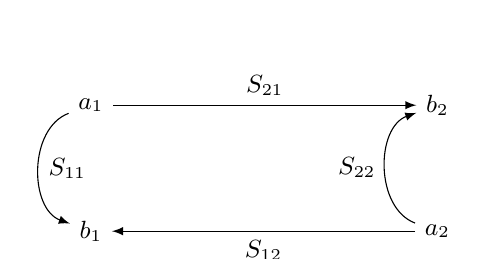
\begin{tikzpicture}[>=latex,every node/.style={font=\small}]
    \node (a1) at (0,1.6) {$a_1$};
    \node (b2) at (4.4,1.6) {$b_2$};
    \node (b1) at (0,0) {$b_1$};
    \node (a2) at (4.4,0) {$a_2$};
    \draw[->] (a1) -- node[above] {$S_{21}$} (b2);
    \draw[->] (a2) -- node[below] {$S_{12}$} (b1);
    \draw[->] (a1) to[bend right=70] node[right,pos=0.5] {$S_{11}$} (b1);
    \draw[->] (a2) to[bend left=70] node[left,pos=0.5] {$S_{22}$} (b2);
  \end{tikzpicture}
  \caption*{The \textbf{graphe de fluence} (\textit{signal-flow graph}) of a
  quadripôle.}
\end{figure}

\begin{prop}[Quelques caractéristiques]
  Un quadripôle est
  \begin{subpart}
    \item \textbf{adapté} si $S_{ii} = 0$ ;
    \item \textbf{réciproque} (\textit{reciprocal}) si $S_{ij} = S_{ji}$ ;
    \item \textbf{symétrique} (\textit{symmetric}) si $S_{ii} = S_{jj}$ \emph{et}
      $S_{ij} = S_{ji}$ ;
    \item \textbf{passif} (\textit{passive}) si tous les paramètres S vérifient
      $|S| \le 1$ ;
    \item \textbf{actif} (\textit{active}) si au moins un des paramètres S est
      supérieur à $1$.
  \end{subpart}
\end{prop}

\subsubsection{Mesure des paramètres S}
Pour caractériser un multipôle par ses paramètres S, il faut alimenter, par un
générateur avec une impédance interne adaptée, l'un des accès qui servira de référence
et fermer les autres accès par une impédance de charge adaptée. Sweeping which accès is
fed and which are terminated fills the matrix column by column. En pratique on réalise
la mesure à l'aide d'un analyseur de réseaux vectoriel (VNA), which is vectorial
precisely because it recovers the phase of $a$ and $b$ that a scalar wattmètre would
throw away.

\subsection{Adaptation d'impédance et paramètres S}
This example chains everything in the chapter: the measured $S_{11}$ of an antenne is
read as a facteur de réflexion, converted into an impedance, modelled by éléments
localisés, cancelled by a parallel reactance and finally transformed by a $\lambda/4$
line.

\begin{figure}[h!]
  \centering
  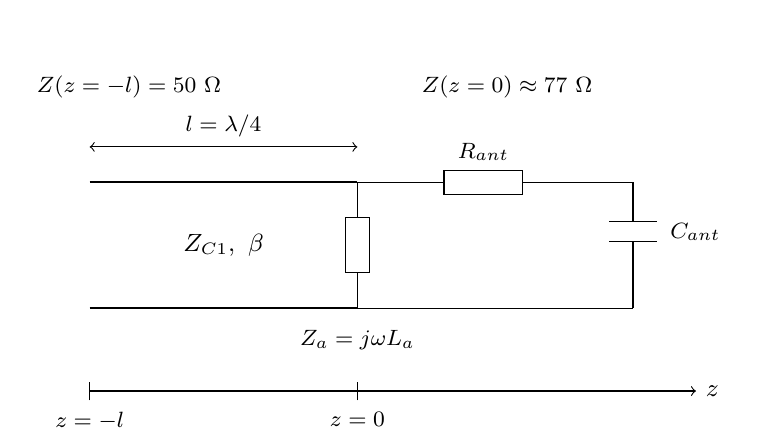
\begin{tikzpicture}[every node/.style={font=\small}]
    % quarter-wave line
    \draw[thick] (0,0.8) -- (3.4,0.8);
    \draw[thick] (0,-0.8) -- (3.4,-0.8);
    \node at (1.7,0) {$Z_{C1},\ \beta$};
    \draw[<->] (0,1.25) -- (3.4,1.25);
    \node[above,font=\footnotesize] at (1.7,1.25) {$l = \lambda/4$};
    % shunt inductance at z = 0
    \draw (3.4,0.8) -- (3.4,0.35);
    \draw (3.25,-0.35) rectangle (3.55,0.35);
    \draw (3.4,-0.35) -- (3.4,-0.8);
    \node[font=\footnotesize] at (3.4,-1.2) {$Z_a = j\omega L_a$};
    % antenna model
    \draw (3.4,0.8) -- (4.5,0.8);
    \draw (3.4,-0.8) -- (6.9,-0.8);
    \draw (4.5,0.65) rectangle (5.5,0.95);
    \node[above,font=\footnotesize] at (5.0,0.95) {$R_{ant}$};
    \draw (5.5,0.8) -- (6.9,0.8) -- (6.9,0.3);
    \draw (6.6,0.3) -- (7.2,0.3);
    \draw (6.6,0.05) -- (7.2,0.05);
    \node[right,font=\footnotesize] at (7.25,0.17) {$C_{ant}$};
    \draw (6.9,0.05) -- (6.9,-0.8);
    % axis
    \draw[->] (0,-1.85) -- (7.7,-1.85) node[right] {$z$};
    \draw (0,-1.97) -- (0,-1.73);
    \draw (3.4,-1.97) -- (3.4,-1.73);
    \node[below,font=\footnotesize] at (0,-2.0) {$z = -l$};
    \node[below,font=\footnotesize] at (3.4,-2.0) {$z = 0$};
    \node[above,font=\footnotesize] at (0.5,1.75) {$Z(z=-l) = 50\ \Omega$};
    \node[above,font=\footnotesize] at (5.3,1.75) {$Z(z=0) \approx 77\ \Omega$};
  \end{tikzpicture}
  \caption*{The quadripôle d'adaptation $Q$: the parallel inductance $L_a$ makes $Z(z=0)$
  real, and the $\lambda/4$ section of impedance $Z_{C1}$ then transforms
  $77\ \Omega$ into $50\ \Omega$. La longueur entre $Z_{ant}$ et l'accès en sortie du
  quadripôle $Q$ est nulle.}
\end{figure}

\begin{example}[Antenne à $1\ \mathrm{GHz}$, $S_{11} = 0.3\,e^{-j60^{\circ}}$, $Z_0 = 50\ \Omega$]
  \textbf{L'antenne est-elle adaptée ?} Le module $|S_{11}| = 0.3 \neq 0$. L'antenne
  n'est donc pas adaptée et une partie de la puissance sera perdue par réflexion.

  \medskip
  \textbf{Impédance d'entrée.} L'antenne est un dispositif à un seul accès, on peut
  donc dire que $\Gamma_{ant} = S_{11}$ avec comme impédance de référence
  $Z_0 = 50\ \Omega$, et
  \[\Gamma_{ant} = S_{11} = \frac{Z_{ant} - Z_0}{Z_{ant} + Z_0}
    \quad\Longrightarrow\quad
    Z_{ant} = Z_0\,\frac{1 + S_{11}}{1 - S_{11}}.\]
  Avec $S_{11} = 0.3\,e^{-j60^{\circ}} = 0.15 - j\,0.26$, on obtient alors
  \[Z_{ant} = R_{ant} + j X_{ant} = 58 - j\,32.9\ \Omega.\]
  La réactance en série est négative, ce qui signifie ici que le composant est une
  capacité, $X_{ant} = -1/(C_{ant}\omega)$, d'où
  \[C_{ant} = \frac{1}{32.9 \times 2\pi \times 10^{9}} = 4.83\ \mathrm{pF}.\]
  Par conséquent l'antenne est modélisée par une résistance $R_{ant} = 58\ \Omega$ en
  série avec une capacité $C_{ant} = 4.83\ \mathrm{pF}$ pour une fréquence de
  fonctionnement fixée à $1\ \mathrm{GHz}$.

  \medskip
  \textbf{Pourquoi il faut ajouter une réactance $Z_a$.} Cette réactance va permettre
  d'annuler la partie imaginaire de $Z_{ant}$ : l'impédance
  $Z(z=0) = Z_{ant} \parallel Z_a$ sera donc réelle, ce qui est obligatoire pour
  réaliser une adaptation par transformateur d'impédance réalisé grâce à une ligne sans
  pertes de longueur $\lambda/4$. Pour éliminer l'effet capacitif de l'antenne, on doit
  donc connecter en parallèle un élément inductif, $Z_a = jX = j\omega L_a$.
  L'admittance formée par l'association en parallèle est égale à
  \[Y(z=0) = Y_{ant} + Y_a
    = \frac{1}{R_{ant} + 1/(j\omega C_{ant})} + \frac{1}{j\omega L_a}
    = \frac{1}{1 + \omega^2 R_{ant}^2 C_{ant}^2}
      \left(\omega^2 R_{ant} C_{ant}^2
        + j\,\frac{L_a C_{ant}\omega^2 - 1}{\omega L_a}\right).\]
  On doit annuler la partie imaginaire, c'est-à-dire que $L_a C_{ant}\omega^2 = 1$,
  soit
  \[L_a = \frac{1}{C_{ant}\,\omega^2} = 5.24\ \mathrm{nH}.\]

  \medskip
  \textbf{Le transformateur d'impédance $\lambda/4$.} Après l'ajout de cette
  inductance, l'admittance $Y(z=0)$ sera purement réelle et
  \[Z(z=0) = \frac{1}{Y(z=0)}
    = \frac{1 + \omega^2 R_{ant}^2 C_{ant}^2}{\omega^2 R_{ant} C_{ant}^2}
    \approx 77\ \Omega.\]
  Le tronçon de ligne ajouté, sans pertes, de longueur $l = \lambda/4$, aura une
  impédance caractéristique choisie de telle sorte que l'impédance ramenée soit
  $Z(z=-l) = Z_{C1}^2/Z(z=0) = 50\ \Omega$, d'où
  \[\begin{cases}
      Z_{C1} = \sqrt{Z(z=0)\,Z(z=-l)} = \sqrt{77 \times 50} = 62\ \Omega \\[1ex]
      l = \dfrac{\lambda}{4} = \dfrac{c}{4 f \sqrt{\varepsilon_r}} = 7.5\ \mathrm{cm}
    \end{cases}\]
  pour une permittivité relative $\varepsilon_r = 1$ de la ligne ajoutée. The complete
  quadripôle d'adaptation $Q$ is thus a $5.24\ \mathrm{nH}$ inductance in parallel at
  $z = 0$, followed by $7.5\ \mathrm{cm}$ of $62\ \Omega$ line.
\end{example}

\begin{remark}
  L'impédance d'entrée de l'antenne est modélisée par une résistance $R_{ant}$ et une
  réactance $jX_{ant}$ placées en série à l'abscisse $z = 0$ ; ceci est un modèle où les
  longueurs de ligne entre elles et le plan d'accès sont nulles. That idealisation is
  what makes $Z_{ant} = Z_0(1+S_{11})/(1-S_{11})$ directly usable: as soon as a length of line
  sits between the components and the reference plane, the phase of $S_{11}$ --- and
  with it the extracted $R$ and $X$ --- changes, which is the «~les paramètres S
  dépendent du plan de référence choisi~» caveat made concrete.
\end{remark}

\section{Antennes, rayonnement, bilan de liaison}
Une antenne assure la conversion d'une onde électromagnétique \emph{guidée} en
une onde électromagnétique \emph{rayonnée} et inversement. Everything upstream
of it --- the generator, the line, the matching network --- has been engineered
so that the power arrives at the terminals of the antenne; une antenne à
l'émission doit répartir dans l'espace toute la puissance tirée du générateur,
en respectant une loi d'éclairement et une orientation des champs donnée. Three
quantities describe it completely enough to read a datasheet. On définit ainsi
trois caractéristiques essentielles pour l'antenne à l'émission :
l'\textbf{impédance d'entrée} (\textit{input impedance}) que présente l'antenne
au générateur et qui conditionne l'adaptation en puissance indispensable pour
extraire du générateur toute la puissance disponible ; le \textbf{diagramme de
rayonnement} (\textit{radiation pattern}), qui définit la répartition spatiale
de la puissance rayonnée ; la \textbf{polarisation}, qui spécifie l'orientation
du champ rayonné et son évolution en fonction du temps. The chapter closes with
the \emph{bilan de liaison}, which is the one calculation in this part the
course insists must be manipulated fluently.

\subsection{Le point sur les unités}

\begin{definition}[Décibel]
  Par définition, le \textbf{décibel} (dB) permet de quantifier un
  \emph{rapport de puissances} en échelle logarithmique,
  \[ G_{\mathrm{dB}} = 10 \log \frac{P_2}{P_1}. \]
  Il est utilisé pour exprimer le gain d'un amplificateur, l'atténuation d'un
  milieu, le gain d'une antenne --- of anything dimensionless.
\end{definition}

\begin{example}[Amplifier]
  An amplifier takes $P_1 = 2$~mW to $P_2 = 1$~W. Gain de l'amplificateur :
  $G = P_2/P_1 = 500$, sans unité ; gain de l'amplificateur en dB :
  $G_{\mathrm{dB}} = 10 \log 500 = 27$~dB.
\end{example}

\begin{definition}[dBm et dBW]
  Une puissance peut être exprimée en dBW ou dBm. Dans ce cas, la puissance est
  définie par rapport à une puissance de référence $P_{\mathrm{ref}}$ :
  \[ P_{\mathrm{dBm}} = 10 \log \frac{P}{1\ \mathrm{mW}}, \qquad
     P_{\mathrm{dBW}} = 10 \log \frac{P}{1\ \mathrm{W}}. \]
  Exemples : $1$~mW, soit $0$~dBm et $-30$~dBW ; $2$~mW, soit $3$~dBm et
  $-27$~dBW ; $1$~W, soit $0$~dBW.
\end{definition}

Since a dB is a ratio and a dBm is a power, only some combinations are legal.
This is exam bookkeeping and is worth memorising as a table rather than
re-deriving each time.

\begin{center}
  \begin{tabular}{@{}ll@{}}
    \toprule
    Opération & Résultat \\
    \midrule
    dB $+$ dB, \quad dB $-$ dB & dB \\
    dBm $+$ dB & dBm \\
    dBm $-$ dB & dBm \\
    dBm $-$ dBm & dB \\
    \midrule
    dBm $+$ dBm & pas possible \\
    dB $-$ dBm & pas possible \\
    \bottomrule
  \end{tabular}
\end{center}

\subsection{D'où vient le rayonnement ?}

\begin{definition}[Antenne]
  Une \textbf{antenne} (\textit{antenna}) est un dispositif qui assure la
  conversion d'une onde électromagnétique guidée en une onde électromagnétique
  rayonnée et inversement.
\end{definition}

Une antenne est donc reliée physiquement à un dispositif de guidage des ondes.
Il peut s'agir d'un câble coaxial, d'une ligne imprimée (ligne coplanaire,
ligne microruban, \ldots) ou d'un guide d'ondes.\\

On peut montrer qu'il existe des champs électriques et magnétiques produits en
un point $M$ de l'espace libre, par des répartitions de courants et de charges
localisées dans un volume $V'$. Les mouvements accélérés des charges sur
l'antenne créent un champ électromagnétique. Ainsi, \emph{seules les sources
(densités de courant) variables dans le temps rayonnent}. Le champ
électromagnétique se propage à la vitesse de la lumière (dans l'air ou le
vide) : $c = 3 \times 10^8$~m$\cdot$s$^{-1}$.

\begin{figure}[h!]
  \centering
  \begin{tikzpicture}[>=latex,scale=1.0]
    \draw[->] (0,0) -- (0,1.9) node[left] {$z$};
    \draw[->] (0,0) -- (2.4,0) node[below] {$y$};
    \draw[->] (0,0) -- (-1.05,-0.95) node[below] {$x$};
    \draw[thick] (5.0,0.9) ellipse (1.05 and 0.78);
    \node at (5.0,-0.15) {\small $V'$ --- antenne};
    \fill (4.85,0.95) circle (1.3pt);
    \node[below] at (4.9,0.92) {\small $M'$};
    \node[right] at (6.15,1.15) {\small $\v{j}(\v{r}',t),\ \rho(\v{r}',t)$};
    \fill (5.9,3.1) circle (1.3pt);
    \node[above right] at (5.9,3.1) {\small $M$};
    \node[left] at (5.85,3.2) {\small $\v{E}(\v{r},t),\ \v{H}(\v{r},t)$};
    \draw[->] (0,0) -- (5.84,3.06) node[pos=0.62,above,sloped] {\small $\v{r}$};
    \draw[->] (0,0) -- (4.80,0.93) node[pos=0.6,below,sloped] {\small $\v{r}'$};
    \draw[->] (4.85,0.95) -- (5.86,3.06) node[pos=0.55,right] {\small $\v{r}-\v{r}'$};
  \end{tikzpicture}
\end{figure}

\begin{remark}[Retarded time]
  Le champ électromagnétique en $M$ à l'instant $t$ dépend de l'état des
  sources à l'instant \emph{antérieur}
  \[ t' = t - \frac{\|\v{r} - \v{r}'\|}{c}, \]
  which is what makes the radiated field a propagating object rather than an
  instantaneous one.
\end{remark}

Les équations de Maxwell permettent de relier le champ électromagnétique et les
courants/charges. The course writes them with $\operatorname{rot}$ and
$\operatorname{div}$:
\[
  \curl \v{E} = -\frac{\del \v{B}}{\del t}, \qquad
  \curl \v{H} = \v{j} + \frac{\del \v{D}}{\del t}, \qquad
  \div \v{D} = \rho, \qquad \div \v{B} = 0,
\]
dans le vide : $\v{B} = \mu_0 \v{H}$ et $\v{D} = \epsilon_0 \v{E}$. La
connaissance des courants sur l'antenne permet donc le calcul du champ
électromagnétique rayonné : $\{\v{j}, \rho\} \lra \{\v{E}, \v{H}\}$.

\begin{remark}[Design constraints]
  Electrical performance is only one constraint. Pour qu'une antenne présente
  de « bonnes » performances, ses dimensions sont de l'ordre de la
  demi-longueur d'onde --- pour les fréquences LTE autour de 700~MHz, la
  longueur d'onde est égale à 43~cm, so $\lambda/2 \approx 21.5$~cm, which is
  why small multiband terminal antennes are hard. Les antennes doivent être
  discrètes et petites pour des raisons esthétiques, mais parfois aussi pour
  des raisons aérodynamiques. Une antenne doit parfois, si son environnement
  l'exige, être capable de fonctionner sur une grande gamme de température
  (typiquement $-120$ à $+120\,^\circ$C sur un satellite) et/ou supporter de
  fortes puissances (kW sur un radar d'aéroport).
\end{remark}

\subsection{Impédance d'entrée de l'antenne}

L'impédance d'entrée de l'antenne est une grandeur complexe :
$Z_{\mathrm{ant}} = R_{\mathrm{ant}} + j X_{\mathrm{ant}}$. L'impédance de
sortie de l'émetteur, $50\ \Omega$, is the usual reference.

\begin{definition}[Facteur de réflexion à l'entrée de l'antenne]
  Le \textbf{facteur de réflexion} du signal à l'entrée de l'antenne est
  \[ \Gamma_{\mathrm{ant}} = \frac{Z_{\mathrm{ant}} - Z_C}{Z_{\mathrm{ant}} + Z_C}, \]
  où $Z_C$ est l'impédance caractéristique de la ligne d'accès à l'antenne
  (câble coaxial, guide d'ondes, \ldots). $\Gamma_{\mathrm{ant}}$ est une
  grandeur complexe ; c'est le rapport entre la tension réfléchie et la
  tension incidente à l'entrée de l'antenne.
\end{definition}

Lorsque $Z_{\mathrm{ant}} = Z_C$, il n'y a pas de réflexion à l'entrée de
l'antenne. C'est le cas idéal. Malheureusement, l'impédance $Z_{\mathrm{ant}}$
dépend de la fréquence ; d'autre part, les caractéristiques d'une antenne et
donc son impédance d'entrée dépendent de l'environnement. On ne peut donc
obtenir un facteur de réflexion nul sur toute la bande souhaitée quel que soit
l'environnement. Néanmoins, le travail du concepteur d'antenne consiste à le
minimiser.\\

Because $\Gamma$ is a voltage ratio, le rapport entre la puissance réfléchie et
la puissance incidente (c'est-à-dire la puissance issue du générateur si on
considère une ligne d'accès sans pertes) s'écrit
$|\Gamma_{\mathrm{ant}}|^2 = P_{\mathrm{refl}} / P_{\mathrm{gen}}$. La
puissance transmise à l'antenne est donc

\[ \boxed{P_{\mathrm{ant}} = \bigl(1 - |\Gamma_{\mathrm{ant}}|^2\bigr) P_{\mathrm{gen}}.} \]

$P_{\mathrm{ant}}$ n'est \emph{pas} la puissance rayonnée : il existe d'autres
pertes au niveau de l'antenne (pertes métalliques, diélectriques, \ldots).

\begin{definition}[Efficacité de rayonnement]
  Avec $e_{\mathrm{ray}}$ l'\textbf{efficacité de rayonnement}
  (\textit{radiation efficiency}), $0 < e_{\mathrm{ray}} < 1$, la puissance
  rayonnée par l'antenne s'écrit
  \[ P_{\mathrm{ray}} = e_{\mathrm{ray}} P_{\mathrm{ant}}, \qquad
     P_{\text{dissipée}} = (1 - e_{\mathrm{ray}}) P_{\mathrm{ant}}. \]
\end{definition}

\begin{figure}[h!]
  \centering
  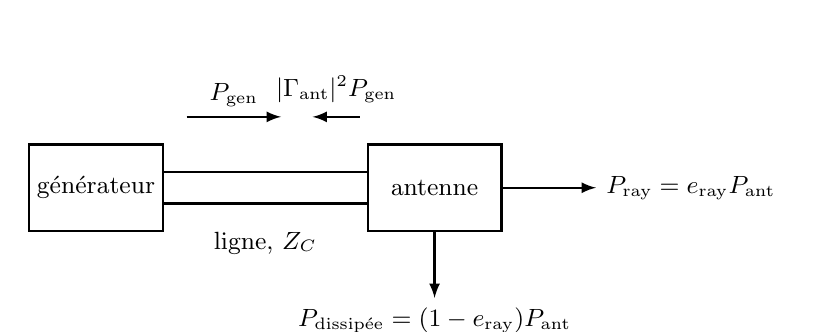
\begin{tikzpicture}[>=latex,scale=1.0]
    \draw[thick] (0,0) rectangle (1.7,1.1);
    \node[align=center] at (0.85,0.55) {\small générateur};
    \draw[thick] (1.7,0.75) -- (4.3,0.75);
    \draw[thick] (1.7,0.35) -- (4.3,0.35);
    \node[align=center] at (3.0,-0.15) {\small ligne, $Z_C$};
    \draw[thick] (4.3,0) rectangle (6.0,1.1);
    \node[align=center] at (5.15,0.55) {\small antenne};
    \draw[->,thick] (2.0,1.45) -- (3.2,1.45) node[midway,above] {\small $P_{\mathrm{gen}}$};
    \draw[<-,thick] (3.6,1.45) -- (4.2,1.45);
    \node[above] at (3.9,1.5) {\small $|\Gamma_{\mathrm{ant}}|^2 P_{\mathrm{gen}}$};
    \draw[->,thick] (6.0,0.55) -- (7.2,0.55) node[right] {\small $P_{\mathrm{ray}} = e_{\mathrm{ray}} P_{\mathrm{ant}}$};
    \draw[->,thick] (5.15,0) -- (5.15,-0.85) node[below] {\small $P_{\text{dissipée}} = (1-e_{\mathrm{ray}})P_{\mathrm{ant}}$};
  \end{tikzpicture}
\end{figure}

\subsubsection{Bande passante}

Les caractéristiques d'une antenne et donc son facteur de réflexion
$\Gamma_{\mathrm{ant}}$ dépendent de la fréquence. Il est donc nécessaire
d'observer les performances d'une antenne sur la ou les bandes de fréquences
d'utilisation. En échelle logarithmique,
\[ |\Gamma_{\mathrm{ant}}|_{\mathrm{dB}} = 20 \log |\Gamma_{\mathrm{ant}}|, \]
the factor $20$ being there because le facteur de réflexion $\Gamma$ est un
rapport de tension et non de puissance.

\begin{remark}[Voltage ratio, not power ratio]
  The factor $20$ is what a voltage ratio calls for; were $\Gamma$ a ratio of
  powers, its expression in dB would carry a factor ten instead.
\end{remark}

\begin{definition}[Bande passante en adaptation]
  Il existe de nombreuses définitions de la bande passante. La plus commune est
  la \textbf{bande passante en adaptation} (\textit{matching bandwidth}), où le
  module du facteur de réflexion de l'antenne $|\Gamma_{\mathrm{ant}}|$ est
  inférieur à un certain niveau (généralement $-10$~dB).
\end{definition}

\begin{example}[Antenne de téléphonie mobile]
  For one commercial antenne, en prenant comme critère
  $|\Gamma_{\mathrm{ant}}|_{\mathrm{dB}} < -6$~dB, valeur typique pour des
  antennes de téléphone mobile, les bandes passantes mesurées sont
  $[700 - 960]$~MHz, $[1.75 - 2.3]$~GHz, $[2.56 - 2.65]$~GHz et
  $[3.1 - 4.38]$~GHz. Cette antenne couvre donc les standards GSM900/1800,
  PCS1900, UMTS2100 et LTE700/2300/2600/3400/3600.
\end{example}

\subsubsection{Rapport d'ondes stationnaires}

\begin{definition}[ROS / VSWR]
  Pour caractériser une antenne en adaptation, au lieu d'étudier
  $|\Gamma_{\mathrm{ant}}|_{\mathrm{dB}}$ dans la bande de fréquences souhaitée,
  on utilise parfois le rapport d'onde stationnaire (ROS) ou VSWR (Voltage
  Standing Wave Ratio) :
  \[ \mathrm{ROS} = \mathrm{VSWR} = \frac{1 + |\Gamma_{\mathrm{ant}}|}{1 - |\Gamma_{\mathrm{ant}}|},
     \qquad\text{equivalently}\qquad
     |\Gamma_{\mathrm{ant}}| = \frac{\mathrm{ROS} - 1}{\mathrm{ROS} + 1}. \]
  Un ROS de $2$ correspond à $|\Gamma_{\mathrm{ant}}|_{\mathrm{dB}} = -9.5$~dB.
\end{definition}

\begin{problem}[Critère d'adaptation d'une antenne]
  Vous recherchez une antenne adaptée dans la bande $3.1 - 5$~GHz. Le système
  sur lequel vous voulez l'intégrer requiert un $\mathrm{ROS} < 2$. Un
  constructeur vous propose une antenne et vous fournit la courbe du module du
  facteur de réflexion $|\Gamma|$ en fonction de la fréquence. Cette antenne
  répond-elle à vos besoins ? Supposons que votre chaîne de transmission
  requiert un $\mathrm{ROS} < 1.4$ : mêmes questions.
\end{problem}

\begin{proof}
  Convert the criterion into a level on the supplied curve. On calcule la
  valeur du module du facteur de réflexion correspondant à un
  $\mathrm{ROS} = 2$ :
  \[ |\Gamma| = \frac{2-1}{2+1} = \frac{1}{3}, \qquad
     |\Gamma|_{\mathrm{dB}} = 20 \log \tfrac{1}{3} = -9.5\ \mathrm{dB}. \]
  La bande passante de l'antenne est l'intervalle de fréquences dans lequel
  $|\Gamma|_{\mathrm{dB}} \le -9.5$~dB. On the supplied curve, la bande passante
  de l'antenne est donc $[3.1 - 5]$~GHz soit $1.9$~GHz. L'antenne répond au
  cahier des charges pour la bande passante.\\

  On suppose un $\mathrm{ROS} = 1.4$ : $|\Gamma| = 0.4/2.4 = 1/6$ et
  $|\Gamma|_{\mathrm{dB}} = -15.6$~dB. Avec le nouveau critère, la bande
  passante est de $500$~MHz comprise dans l'intervalle $[4.25 - 4.75]$~GHz, ce
  qui ne convient donc plus au cahier des charges demandé. \qed
\end{proof}

\subsection{Diagramme de rayonnement}

Le diagramme de rayonnement est une représentation graphique de la répartition
spatiale de la puissance rayonnée par l'antenne.

\subsubsection{Champ lointain et coordonnées sphériques}

\begin{definition}[Champ lointain]
  Pour tracer un diagramme de rayonnement, on s'intéresse au rayonnement en
  \textbf{champ lointain} (\textit{far field}), c'est-à-dire loin des sources
  (antenne). En général, la zone de champ lointain est située au-delà d'une
  distance, appelée \textbf{distance de Fraunhofer}
  (\textit{Fraunhofer distance}),
  \[ r > \frac{2 D^2}{\lambda}, \]
  $D$ étant la plus grande dimension de l'antenne et $\lambda$ la longueur
  d'onde.
\end{definition}

Dans la zone de champ lointain, les ondes électromagnétiques se propageant sont
des ondes \emph{sphériques}. L'amplitude des champs $\v{E}$ et $\v{H}$ varie en
$1/r$. Localement, l'onde pourra être considérée comme plane, so that the ratio
of the field magnitudes is the impédance d'onde du vide
\[ \frac{E}{H} = \eta_0 = \sqrt{\frac{\mu_0}{\epsilon_0}} = 120\pi = 377\ \Omega. \]
Les coordonnées sphériques $(r, \theta, \varphi)$ sont souvent utilisées pour
tracer le diagramme de rayonnement, $\theta$ being the angle from $Oz$ and
$\varphi$ the azimuth in $xOy$.

\subsubsection{Densité surfacique de puissance et puissance rayonnée}

La puissance d'une onde électromagnétique s'exprime par le vecteur de Poynting.
La moyenne temporelle du vecteur de Poynting en régime harmonique en $M$
s'écrit
\[ \v{\Pi}(r,\theta,\varphi) = \frac{\Re\bigl(\v{E} \wedge \v{H}^{*}\bigr)}{2}, \]
and its norm $p(r,\theta,\varphi) = \|\v{\Pi}(r,\theta,\varphi)\|$, en
W$/$m$^2$, représente la \textbf{densité de puissance surfacique} au point
$M$.

\begin{definition}[Puissance totale rayonnée]
  La \textbf{puissance totale rayonnée} (\textit{total radiated power}) est
  égale au flux du vecteur de Poynting à travers une sphère de rayon $r$
  entourant l'antenne :
  \[ P_{\mathrm{ray}} = \oint\!\!\!\!\oint_{\text{sphère}} \v{\Pi} \cdot \mathrm{d}\v{S}
     = \int_{\theta=0}^{\pi} \int_{\varphi=0}^{2\pi}
       p(r,\theta,\varphi)\, r^2 \sin\theta \,\mathrm{d}\theta\, \mathrm{d}\varphi. \]
\end{definition}

\subsubsection{Directivité et gain d'une antenne}

Pour quantifier l'aptitude d'une antenne à rayonner l'énergie dans une
direction donnée, on la compare à l'\textbf{antenne isotrope}
(\textit{isotropic antenna}), c'est-à-dire à une antenne qui rayonne toute son
énergie de manière uniforme dans tout l'espace. La densité surfacique de
puissance de l'antenne isotrope est donc
\[ p_{\mathrm{iso}}(r) = \frac{P_{\mathrm{ray}}}{4\pi r^2}. \]

\begin{definition}[Directivité et gain]
  La \textbf{directivité} (\textit{directivity}) et le \textbf{gain} d'une
  antenne sont définis par
  \[ D(\theta,\varphi) = \frac{p(r,\theta,\varphi)}{p_{\mathrm{iso}}(r)}
     = \frac{p(r,\theta,\varphi)}{P_{\mathrm{ray}}}\, 4\pi r^2,
     \qquad
     G(\theta,\varphi) = \frac{p(r,\theta,\varphi)}{P_{\mathrm{ant}}}\, 4\pi r^2
     = e_{\mathrm{ray}} D(\theta,\varphi). \]
  La directivité s'exprime généralement en dBi ($i$ : isotrope),
  $D(\theta,\varphi)_{\mathrm{dBi}} = 10 \log D(\theta,\varphi)$ ; le gain
  s'exprime plutôt en dB, ou en dBi.
\end{definition}

\begin{remark}
  The directivité is normalised by construction: la directivité d'une antenne
  \emph{ne peut} être supérieure à $1$ dans toutes les directions. Une
  directivité élevée dans une direction donnée est obtenue au détriment des
  autres directions. The distinction between $D$ and $G$ is exactly the
  efficacité de rayonnement, qui représente les pertes dans l'antenne (pertes
  métalliques et diélectriques).
\end{remark}

\subsubsection{Les différentes représentations graphiques du diagramme de rayonnement}

Le \emph{diagramme en 3D}, plotting $D$ or $G$ in dB over the sphere, apporte
une information essentiellement qualitative sur les directions de rayonnement
ou d'absence de rayonnement. Afin d'obtenir une information plus quantitative,
on réalise des \textbf{plans de coupe} (\textit{cutting plane}) à partir du
diagramme 3D, for instance $\varphi = 0$ ; le diagramme dans un plan peut être
tracé en coordonnées polaires ou cartésiennes.

\begin{figure}[h!]
  \centering
  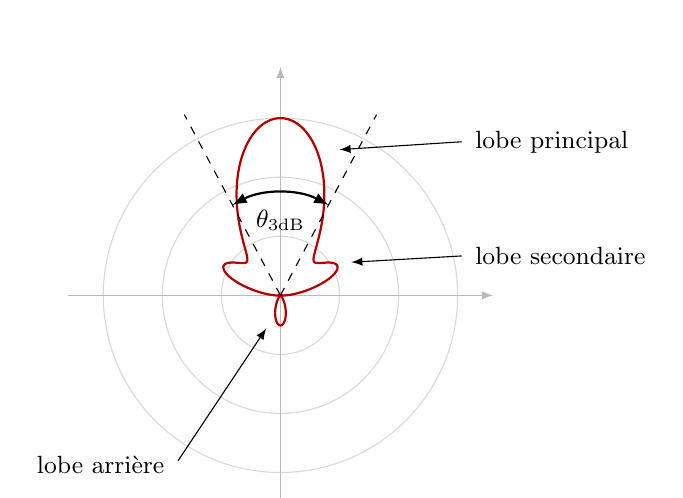
\begin{tikzpicture}[>=latex,scale=1.0]
    \foreach \rr in {0.75,1.5,2.25} { \draw[gray!30] (0,0) circle (\rr); }
    \draw[gray!55,->] (-2.7,0) -- (2.7,0);
    \draw[gray!55,->] (0,-2.7) -- (0,2.9);
    \draw[thick,red!70!black,samples=361,domain=-180:180,smooth]
      plot ({\x+90}:{2.25*(exp(-((\x)/34)^2) + 0.33*exp(-((\x-64)/17)^2)
        + 0.33*exp(-((\x+64)/17)^2) + 0.17*exp(-((\x-180)/24)^2)
        + 0.17*exp(-((\x+180)/24)^2))});
    \draw[dashed] (0,0) -- (62:2.6);
    \draw[dashed] (0,0) -- (118:2.6);
    \draw[<->,thick] (62:1.3) arc (62:118:1.3);
    \node at (0,0.95) {\small $\theta_{3\mathrm{dB}}$};
    \node[align=center,right] at (2.35,1.95) {\small lobe principal};
    \draw[->] (2.3,1.95) -- (0.75,1.85);
    \node[align=center,right] at (2.35,0.5) {\small lobe secondaire};
    \draw[->] (2.3,0.5) -- (0.9,0.42);
    \node[align=center,left] at (-1.35,-2.15) {\small lobe arrière};
    \draw[->] (-1.3,-2.1) -- (-0.18,-0.42);
  \end{tikzpicture}
\end{figure}

Le \textbf{lobe principal} (\textit{main lobe}) est défini entre les deux
minima de chaque côté du maximum. Des maxima secondaires apparaissent de chaque
côté. Ils constituent les \textbf{lobes secondaires} (\textit{side lobe}), the
one opposite the main beam being the \textbf{lobe arrière}
(\textit{back lobe}).

\begin{definition}[Ouverture à $-3$~dB]
  L'\textbf{ouverture à $-3$~dB} (\textit{beamwidth}), notée
  $\theta_{3\mathrm{dB}}$, est la plage angulaire sur laquelle
  $G_{\mathrm{dB}} \ge G_{\max,\mathrm{dB}} - 3$~dB. On parle également
  d'ouverture à mi-puissance (HPBW).
\end{definition}

Un diagramme 2D (représentation polaire ou cartésienne) peut également être
\emph{normalisé} par rapport à la directivité (ou gain) maximale. Dans ce cas,
le maximum de la courbe est $0$~dB. On perd alors l'information du gain
maximal $G_{\max}$, mais la lecture des niveaux relatifs entre les lobes est
directe.

\begin{example}[Reading a diagramme de rayonnement]
  A simulated diagramme de rayonnement at $2.18$~GHz, cut at
  $\varphi = 0^\circ$, reports: lobe principal magnitude $5.9$~dBi, lobe
  principal direction $65.0^\circ$, angular width ($3$~dB) $145.8^\circ$, lobe
  secondaire level $-11.2$~dB relative to the peak. The simulator readout
  gives the bare number ``Frequency $= 2.18$'' with no unit; GHz is inferred
  from the context.
\end{example}

\subsection{Polarisation}

La polarisation du champ électromagnétique rayonné par une antenne est donnée
par la \emph{direction du champ électrique}. On considère une propagation
suivant $Oz$ ; de façon générale, le champ électrique s'écrit
\[ \v{E} = \v{E}_x + \v{E}_y, \qquad
   \v{E}_x = E_{0x}\, e^{j(\omega t - kz)}\, \unitv{e}_x, \qquad
   \v{E}_y = E_{0y}\, e^{j(\omega t - kz + \varphi)}\, \unitv{e}_y. \]
The three cases are distinguished entirely by the déphasage $\varphi$ between
the components and by the two amplitudes.

\begin{definition}[Polarisation rectiligne]
  \textbf{Polarisation rectiligne} (\textit{rectilinear polarisation}) ou
  linéaire : la direction du vecteur $\v{E}$ ne varie pas lors de la
  propagation. Au cours du temps, l'extrémité du vecteur décrit une droite dans
  un plan orthogonal à l'axe de propagation. Le déphasage entre les composantes
  est $\varphi = 0$ ou $\varphi = \pi$.
\end{definition}

\begin{definition}[Polarisation circulaire]
  \textbf{Polarisation circulaire} (\textit{circular polarisation}) : la
  direction du vecteur $\v{E}$ varie lors de la propagation. Au cours du temps,
  l'extrémité du vecteur décrit un cercle dans un plan orthogonal à l'axe de
  propagation. This requires
  \[ \varphi = \pm \frac{\pi}{2} \qquad\text{and}\qquad E_{0x} = E_{0y}. \]
  Si $\varphi = -\pi/2$ : \textbf{polarisation circulaire droite}
  (\textit{right-handed}) ; si $\varphi = +\pi/2$ : \textbf{polarisation
  circulaire gauche} (\textit{left-handed}).
\end{definition}

\begin{remark}[The handedness convention]
  Par convention, la polarisation est dite « droite » pour l'observateur qui
  voit \emph{s'éloigner} l'onde, le champ électrique tourne alors dans le sens
  des aiguilles d'une montre (anti-trigonométrique). Elle est dite « gauche »
  dans le cas contraire. The convention is stated with respect to the
  observer, so it must be quoted with its reference or it is meaningless.
\end{remark}

\begin{definition}[Polarisation elliptique]
  \textbf{Polarisation elliptique} (\textit{elliptical polarisation}) : au
  cours du temps, l'extrémité du vecteur $\v{E}$ décrit une ellipse dans un
  plan orthogonal à l'axe de propagation. Le déphasage entre les composantes
  $\varphi$ est quelconque. Polarisation rectiligne and polarisation circulaire
  are its two degenerate cases.
\end{definition}

\begin{definition}[Polarisation croisée (\textit{cross-polarisation})]
  L'antenne peut présenter des défauts et rayonner un champ électrique avec une
  polarisation dégradée. On appelle \textbf{composante principale ou copolaire}
  (\textit{co-polar component}) la composante de champ désirée et
  \textbf{composante croisée} (\textit{cross-polar component}) celle non
  voulue. La composante croisée doit donc être la plus faible possible.
\end{definition}

\begin{example}[Antenne quasi-Yagi]
  For the quasi-Yagi antenne, la polarisation souhaitée est une polarisation
  linéaire suivant la direction des brins, $Ox$, with propagation along $Oz$ ;
  le champ $\v{E}$ est transverse (plan $xOy$). The component along $Ox$ is the
  composante principale ou copolaire, the residual component along $Oy$ is the
  composante croisée.
\end{example}

\subsection{Quelques antennes usuelles}

\subsubsection{Antennes filaires}

Les \textbf{antennes filaires} (\textit{wire antennas}) sont composées d'un ou
plusieurs conducteurs linéaires de diamètre faible. Le diagramme de rayonnement
est calculé à partir de la densité de courant sur l'antenne. Les antennes de
base sont les dipôles, les monopôles, les boucles ; des structures plus
évoluées sont les hélices, les antennes Yagi, les log-périodiques.

\paragraph{Antenne dipôle} Un dipôle est une antenne filaire composée de deux
brins conducteurs et alimentée au centre. La forme la plus courante est le
\textbf{dipôle demi-onde} (\textit{half-wave dipole}) ; la longueur de chaque
brin est dans ce cas égale à $\lambda/4$. La répartition de l'intensité du
courant le long du dipôle demi-onde est
\[ i(z,t) = I_0 \cos\!\left(\frac{2\pi z}{\lambda}\right) e^{j \omega t}, \]
maximal at the feed point and vanishing at the two ends. La polarisation d'un
dipôle est linéaire et le champ électrique $\v{E}$ est parallèle au dipôle.
L'impédance d'entrée du dipôle demi-onde est
\[ Z_{\mathrm{in}} = 73 + j\,42\ \Omega. \]

À grande distance (champ lointain), le champ rayonné peut être calculé :
\[ E_\theta(r,\theta) = -j \frac{60}{r} I_0
     \frac{\cos\left(\frac{\pi}{2}\cos\theta\right)}{\sin\theta}\,
     e^{j(\omega t - kr)},
   \qquad H_\varphi(r,\theta) = \frac{E_\theta(r,\theta)}{Z_0}, \]
avec $Z_0 = 377\ \Omega$ l'impédance d'onde du vide. On peut noter que les
champs sont transverses et que leur amplitude décroît en $1/r$ ; et que les
champs ne dépendent pas de l'angle $\varphi$, ce qui est cohérent avec la
symétrie cylindrique de l'antenne.

\begin{prop}[Directivité du dipôle demi-onde]
  \[ D(\theta) = 1.64 \left(\frac{\cos\left(\frac{\pi}{2}\cos\theta\right)}{\sin\theta}\right)^{2}. \]
  Pour $\theta = \pi/2$, la directivité est maximale :
  $D_{\max} = 1.64$ soit $2.15$~dBi. Pour $\theta = 0$ ou $\pi$, la directivité
  est nulle : un dipôle ne rayonne pas suivant son axe.
\end{prop}

\begin{remark}
  La directivité étant maximale et identique sur un plan (ici le plan $xOy$),
  le rayonnement est dit \textbf{omnidirectionnel} (\textit{omnidirectional})
  --- à ne pas confondre avec \emph{isotrope}. Omnidirectionnel means uniform
  in one plane; isotrope would mean uniform over the whole sphere, and no real
  antenne is isotrope.
\end{remark}

\begin{figure}[h!]
  \centering
  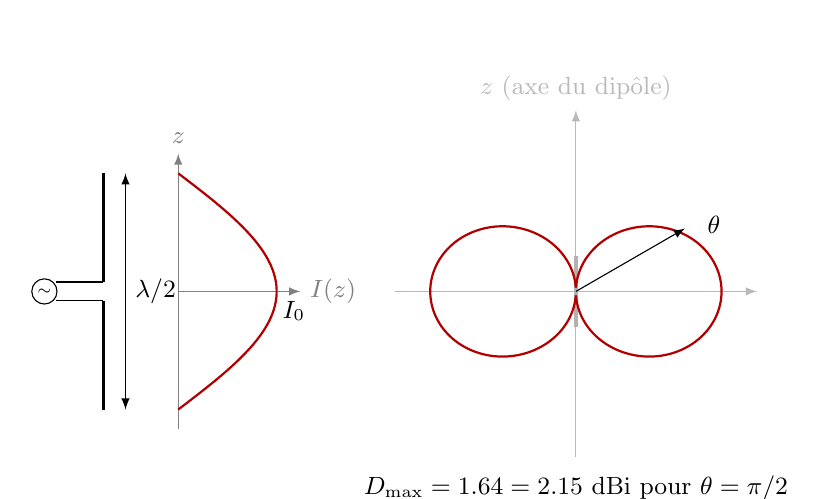
\begin{tikzpicture}[>=latex,scale=1.0]
    % left panel: current distribution
    \begin{scope}[xshift=0cm]
      \draw[very thick] (0,0.12) -- (0,1.5);
      \draw[very thick] (0,-0.12) -- (0,-1.5);
      \draw (0,0.12) -- (-0.45,0.12);
      \draw (0,-0.12) -- (-0.45,-0.12);
      \draw (-0.45,0.12) -- (-0.6,0.12);
      \draw (-0.45,-0.12) -- (-0.6,-0.12);
      \draw (-0.75,0) circle (0.16);
      \node at (-0.75,0) {\tiny $\sim$};
      \draw[<->] (0.28,-1.5) -- (0.28,1.5) node[midway,right] {\small $\lambda/2$};
      \draw[->,gray] (0.95,-1.75) -- (0.95,1.75) node[above] {\small $z$};
      \draw[->,gray] (0.95,0) -- (2.5,0) node[right] {\small $I(z)$};
      \draw[thick,red!70!black,samples=60,domain=-1:1,smooth]
        plot ({0.95+1.25*cos(90*\x)},{1.5*\x});
      \node[below right] at (2.15,0) {\small $I_0$};
    \end{scope}
    % right panel: pattern
    \begin{scope}[xshift=6.0cm]
      \draw[gray!55,->] (0,-2.1) -- (0,2.3) node[above] {\small $z$ (axe du dipôle)};
      \draw[gray!55,->] (-2.3,0) -- (2.3,0);
      \draw[very thick,gray!60] (0,-0.45) -- (0,0.45);
      \draw[thick,red!70!black,samples=180,domain=2:178,smooth]
        plot ({90-\x}:{1.85*abs(cos(90*cos(\x))/sin(\x))});
      \draw[thick,red!70!black,samples=180,domain=2:178,smooth]
        plot ({90+\x}:{1.85*abs(cos(90*cos(\x))/sin(\x))});
      \node[right] at (1.55,0.85) {\small $\theta$};
      \draw[->] (0,0) -- (30:1.6);
      \node at (0,-2.5) {\small $D_{\max} = 1.64 = 2.15$ dBi pour $\theta = \pi/2$};
    \end{scope}
  \end{tikzpicture}
\end{figure}

\paragraph{Antenne monopôle quart d'onde} Une antenne \textbf{monopôle quart
d'onde} (\textit{quarter-wave monopole}) est constituée d'un seul brin de
l'antenne dipôle demi-onde, de longueur $\lambda/4$ et situé au-dessus d'un
plan conducteur qui joue le rôle de réflecteur. Si le plan réflecteur est un
conducteur électrique parfait de dimensions infinies, on peut appliquer le
\emph{principe des images} : le rayonnement dans le demi-espace supérieur est
identique à celui d'un dipôle demi-onde. On note néanmoins que la directivité
augmente de $3$~dB compte-tenu que toute la puissance se trouve uniquement dans
le demi-espace supérieur. Lorsque le plan réflecteur est de dimensions finies
(say a disque de rayon $2\lambda$), la forme du diagramme de rayonnement change
mais la symétrie cylindrique est conservée.

\begin{figure}[h!]
  \centering
  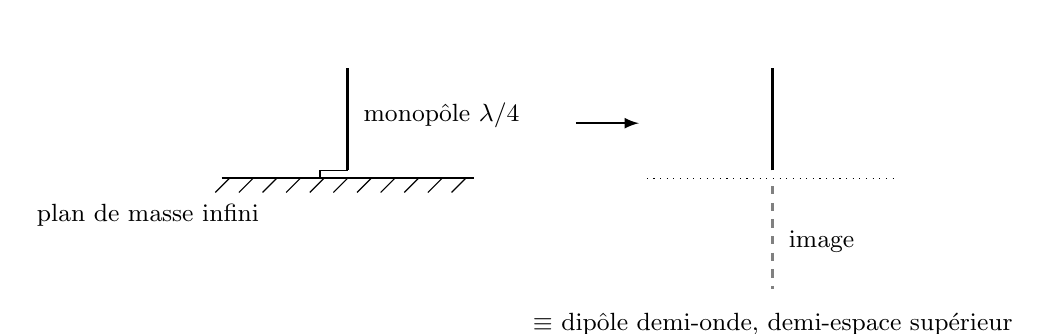
\begin{tikzpicture}[>=latex,scale=1.0]
    \draw[very thick] (0,0.1) -- (0,1.4);
    \node[right] at (0.08,0.8) {\small monopôle $\lambda/4$};
    \draw[thick] (-1.6,0) -- (1.6,0);
    \foreach \x in {-1.5,-1.2,...,1.55} { \draw (\x,0) -- (\x-0.18,-0.18); }
    \node[below left] at (-1.0,-0.2) {\small plan de masse infini};
    \draw (0,0.1) -- (-0.35,0.1) -- (-0.35,0.0);
    \draw[->,thick] (2.9,0.7) -- (3.7,0.7);
    \begin{scope}[xshift=5.4cm]
      \draw[very thick] (0,0.1) -- (0,1.4);
      \draw[very thick,dashed,gray] (0,-0.1) -- (0,-1.4);
      \draw[dotted] (-1.6,0) -- (1.6,0);
      \node[right] at (0.08,-0.8) {\small image};
      \node at (0,-1.85) {\small $\equiv$ dipôle demi-onde, demi-espace supérieur};
    \end{scope}
  \end{tikzpicture}
\end{figure}

\paragraph{Applications des antennes demi-ondes et quart d'ondes} Compte-tenu
de leur rayonnement omnidirectionnel, les antennes demi-ondes et quart d'ondes
sont utilisées pour la diffusion (TNT, radio) et pour les communications
point-multipoints (WiFi, etc.).

\paragraph{Antenne dipôle replié} L'antenne \textbf{dipôle replié}
(\textit{folded dipole}) est constituée de deux dipôles demi-ondes connectés
entre eux aux extrémités et espacés d'une distance très inférieure à la
longueur d'onde. Le dipôle replié a les mêmes caractéristiques que le dipôle
mais une impédance d'entrée plus élevée et une bande passante supérieure ; the
exact increase depends on the diameter of the dipôles and on their spacing. A
VHF example is the DigiTek antenne around $200$~MHz.

\paragraph{Effet d'éléments parasites} Si on place un dipôle \emph{non
alimenté} proche du dipôle initial, on alimente celui-ci par couplage. En
choisissant des tailles légèrement différentes de ces parasites, on peut créer
des comportements \textbf{réflecteur} (\textit{reflector}) ou
\textbf{directeur} (\textit{director}). For example, with a $30$~mm dipôle
actif and a $15$~mm spacing, a $26$~mm parasite acts as a directeur (shorter
than the driven element, beam pulled towards it), a $34$~mm parasite as a
réflecteur (longer, beam pushed away from it). It is thus the $34$~mm element
that gives the comportement réflecteur, and its diagramme de rayonnement is
that of a réflecteur.

\paragraph{Antenne Yagi} L'antenne \textbf{Yagi} (ou Yagi-Uda) comporte un
élément actif (usually a dipôle replié), un réflecteur et un ensemble de
directeurs, dipôles passifs colinéaires. L'objectif est d'obtenir une antenne
large bande et directive. Elle est couramment employée pour la réception de la
télévision.

\begin{center}
  \begin{tabular}{@{}ll@{}}
    \toprule
    Impédance d'entrée & $75\ \Omega$ (grand public) \\
    Gain & $4$~dB pour un directeur, $20$~dB pour 20 directeurs \\
    $\theta_{3\mathrm{dB}}$ & de $60^\circ$ (faible gain) à $25^\circ$ (grand gain) \\
    Rapport avant/arrière & en général $> 25$~dB \\
    \bottomrule
  \end{tabular}
\end{center}

Le \textbf{rapport avant/arrière} (\textit{front-to-back ratio}, AV/AR) est la
différence de niveau de puissance captée par le dipôle pour un signal de même
intensité, en provenance de l'avant et de l'arrière de l'antenne. Une antenne
Yagi commerciale pour la réception TNT, $[470 - 790]$~MHz, quotes
$\theta_{3\mathrm{dB}} = 40^\circ$, $G_{\max} = 15$~dB and AV/AR $= 23$~dB ;
on remarquera que le réflecteur est constitué d'une grille repliée afin de
maximiser l'effet réflecteur et augmenter davantage la directivité.

\subsubsection{Antenne à ouverture rayonnante}

Une \textbf{ouverture rayonnante} (\textit{radiating aperture}) plane est une
ouverture de surface quelconque dans un plan conducteur, illuminé par une onde
incidente. Selon le principe de Huygens, le champ rayonné en un point $P$ est
la superposition du rayonnement de sources secondaires réparties sur
l'ouverture.

\begin{prop}[Directivité maximale d'une ouverture rayonnante]
  En première approximation, il est possible à partir des champs calculés en
  $P$, situé très loin de l'ouverture, d'établir l'expression de la directivité
  maximale de l'ouverture rayonnante :
  \[ D_{\max} = \frac{4 \pi A}{\lambda^2}, \]
  $A$ étant la surface de l'ouverture.
\end{prop}

\paragraph{Antenne cornet} L'\textbf{antenne cornet} (\textit{horn antenna})
est une antenne métallique constituant une transition progressive d'un guide
d'ondes vers l'espace libre. La connaissance du champ dans l'ouverture permet
le calcul du champ lointain. Les avantages des antennes cornets sont un grand
gain, de faibles pertes et une large bande passante --- antenne cornet Hemera,
$[28 - 40]$~GHz, $G = 20$~dB.

\paragraph{Antenne à réflecteur} Une \textbf{antenne à réflecteur}
(\textit{reflector antenna}) est constituée d'une source située au foyer du
réflecteur et d'un réflecteur. Les antennes à réflecteur sont très utilisées
dans les applications nécessitant une antenne directive : liaisons point à
point, réception TV par satellite. Elles présentent plusieurs avantages : un
gain élevé qui augmente avec la surface de l'ouverture du réflecteur,
$D_{\max} = 4\pi A/\lambda^2$ ; la possibilité d'obtenir une couverture ad-hoc
en déformant le réflecteur ; la possibilité d'obtenir plusieurs spots en
plaçant plusieurs sources au niveau du foyer. L'inconvénient majeur de ce type
d'antennes est l'encombrement.

La \textbf{parabole centrée} (\textit{centred parabola}) est constituée d'une
source au foyer et d'un réflecteur parabolique. L'inconvénient majeur est le
masquage d'une partie du faisceau réfléchi par la source et son système
d'alimentation, ce qui détériore l'efficacité de l'antenne et la forme du
diagramme de rayonnement. La \textbf{parabole offset}
(\textit{offset parabola}), ou à foyer décalé, est constituée d'une source
placée au foyer d'un réflecteur qui est une portion de paraboloïde au contour
elliptique. Par rapport à la parabole centrée, le rendement est amélioré,
surtout pour les petites antennes comme celles qui sont utilisées par le grand
public pour la réception de la télévision par satellite. D'autre part, dans
cette géométrie, le réflecteur peut conserver une position quasi verticale même
pour les satellites placés assez haut dans le ciel. Pour rendre plus compacte
une antenne de grande focale, on utilise le montage à double réflecteur de type
\emph{Cassegrain}, qui est commun dans les télescopes : le cornet
d'alimentation se trouve au centre du réflecteur principal et envoie les ondes
vers un réflecteur secondaire hyperbolique convexe --- dont le point focal
arrière coïncide avec le point focal du réflecteur primaire parabolique --- qui
les retourne vers le réflecteur principal. On ajoute ainsi un deuxième
réflecteur, ce qui permet d'augmenter la directivité du système antennaire.

\begin{example}[Parabolic dish at $11$~GHz]
  Pour un réflecteur parabolique, l'ouverture est un disque de rayon $r_d$,
  so $A = \pi r_d^2$ and $D_{\max} = 4\pi A/\lambda^2$. En supposant que
  l'efficacité est de $60\%$, on en déduit les valeurs du gain maximal ;
  enfin, l'ouverture à 3~dB est donnée par la relation
  $\theta_{3\mathrm{dB}} = 70 \lambda / D_o$ (en degrés), avec $D_o$ le
  diamètre de l'ouverture.
  \begin{center}
    \begin{tabular}{@{}lccc@{}}
      \toprule
      Diamètre & $D_{\max}$ & $G_{\max}$ & $\theta_{3\mathrm{dB}}$ \\
      \midrule
      $1.8$~m & $46.3$~dBi & $44.1$~dB & $1^\circ$ \\
      $1.2$~m & $42.8$~dBi & $40.6$~dB & $1.6^\circ$ \\
      \bottomrule
    \end{tabular}
  \end{center}
  Doubling the aperture area buys $3$~dB, and the beam narrows in proportion to
  $\lambda/D_o$: a $1.8$~m dish at $11$~GHz must be pointed to within about a
  degree.
\end{example}

Les antennes à réflecteur sont principalement utilisées sur les satellites,
pour les \textbf{faisceaux hertziens} (\textit{point-to-point microwave links})
terrestres (liaisons point à point), pour la réception TV par satellite ---
parabole offset, $[10.7 - 12.75]$~GHz --- et pour les stations sol
d'émission-réception pour les communications satellitaires, such as the
station sol de O3B, a parabole Cassegrain covering $[17.7 - 20.2]$~GHz.

\subsubsection{Antennes réseaux}

\begin{definition}[Antenne réseau]
  Une \textbf{antenne réseau} (\textit{array antenna}), ou réseau d'antennes,
  est une association de plusieurs éléments rayonnants disposés et excités de
  façon à augmenter le gain dans certaines directions et le réduire dans
  d'autres.
\end{definition}

Les éléments peuvent être alimentés de la même façon ou avec une amplitude et
une phase différente afin de \textbf{dépointer} (\textit{steer}) le faisceau.
Pour créer les lois d'amplitudes et phases voulues, on peut utiliser un réseau
de distribution fixe ou reconfigurable, made of the sources, of
\textbf{déphaseurs} (\textit{phase shifters}) and of atténuateurs ou diviseurs
de puissance, shared between émetteur and récepteur. On distingue les
\textbf{antennes à faisceaux conformés} (\textit{shaped-beam antennas}), les
\textbf{antennes à balayage électronique}
(\textit{electronically scanned antennas}) et les antennes adaptatives.\\

For instance: une antenne réseau planaire à $16$ éléments à faisceau conformé
(système d'alimentation fixe) ; une antenne réseau plan pour un balayage
électronique (un déphaseur par élément rayonnant) ; une antenne réseau avec
sources déphasées individuellement, dépointage dans les 2 plans, with no moving
part. Contemporary examples are a réseau d'antennes en bande Ka around
$30$~GHz, the Satixfy in-flight connectivity terminal using Electronically
Steered Multibeam Antenna (ESMA) technology, and the first-generation Starlink
user terminal.

\subsubsection{Antennes planaires}

\begin{definition}[Antenne microruban]
  Une \textbf{antenne microruban} (\textit{microstrip antenna}), ou antenne
  patch, est constituée d'un élément rayonnant métallique, d'un substrat
  diélectrique et d'un plan de masse.
\end{definition}

La technologie imprimée est intéressante car elle présente un faible coût, un
faible encombrement, une faible masse, la possibilité d'être conformée sur un
support de forme quelconque et une compatibilité avec l'intégration de
composants actifs. Elle a néanmoins des limitations en termes de bande passante
(elle est en général faible), de puissance maximale (celle-ci est limitée à
cause des phénomènes de claquage dans le diélectrique) et de gain, qui est
relativement faible, of the order of $6$~dB. Une antenne microruban peut être
alimentée par une ligne microruban ou un connecteur coaxial.\\

Le \textbf{monopôle imprimé} (\textit{printed monopole}) supprime le plan de
masse sous l'antenne : le rayonnement sera alors comparable à celui d'une
antenne filaire. Le monopôle est alimenté par une ligne microruban constituée
d'un ruban conducteur et d'un plan de masse sur la deuxième face --- il n'y a
pas de plan de masse sur la face en regard de l'antenne ---, et un connecteur
coaxial est soudé sur la ligne microruban, la masse du connecteur étant reliée
au plan de masse de la ligne. Dans cette configuration, le plan de masse de la
ligne microruban agit comme un réflecteur pour le monopôle, et le diagramme de
rayonnement est omnidirectionnel dans le plan orthogonal.

\subsection{Bilan de liaison}

\begin{definition}[Bilan de liaison]
  Le \textbf{bilan de liaison} (\textit{link budget}) is the power accounting
  of a wireless link. Il est indispensable afin de dimensionner une liaison sans
  fil émetteur--récepteur : puissance requise à l'émission, taille des
  antennes, portée.
\end{definition}

Par exemple, on souhaite établir une liaison ayant un signal reçu avec un
\textbf{taux d'erreur binaire} (\textit{bit error rate}) donné. Ce taux dépend
entre autres de la puissance reçue, du bruit au niveau du récepteur, du
traitement de signal effectué et des brouillages éventuels. Dans ce cours, nous
nous intéressons à la puissance reçue $P_R$. Si $P_R$ est inférieure à une
certaine valeur $P_{R,\min}$, appelée \textbf{sensibilité du récepteur}
(\textit{receiver sensitivity}), alors il est impossible d'exploiter le signal
utile. Le calcul de $P_R$ s'effectue à partir des paramètres du système :
caractéristiques du signal à transmettre, caractéristiques de l'émetteur et du
récepteur, milieu environnant.

\subsubsection{Surface équivalente d'une antenne}

Throughout the derivation of the équation de Friis, on suppose que le signal
entre l'antenne d'émission et l'antenne de réception se propage \emph{dans le
vide (ou dans l'air) sans obstacle}. On considère que les deux antennes sont
espacées d'une distance $d$.

\begin{definition}[Surface équivalente d'antenne]
  Une antenne de réception présente au rayonnement provenant de l'antenne
  d'émission une certaine surface $S$ --- par exemple l'ouverture de l'antenne
  parabolique ---, appelée \textbf{surface équivalente d'antenne}
  (\textit{equivalent surface}) ou \textbf{surface de captation}
  (\textit{capture surface}). La puissance reçue est alors donnée par
  \[ P_{R\,[\mathrm{W}]} = p(r,\theta,\varphi)_{[\mathrm{W/m^2}]} \times S_{[\mathrm{m^2}]}, \]
  la direction de la liaison étant définie par les angles $(\theta,\varphi)$.
\end{definition}

Pour une antenne à ouverture rayonnante, sa surface équivalente est
\emph{inférieure ou égale} à la surface de son ouverture. Il existe une
relation qui lie le gain de l'antenne de réception dans la direction de la
liaison à sa surface équivalente :
\[ G_r = \frac{4\pi}{\lambda^2} S. \]

\subsubsection{Équation des télécommunications}

\begin{theorem}[Équation de Friis (\textit{Friis equation}) / Équation des télécommunications]
  Soit $P_e$ la puissance de l'émetteur, $G_e$ le gain de l'antenne d'émission
  dans la direction de la liaison et $G_r$ le gain de l'antenne de réception
  dans la direction de la liaison, les deux antennes étant espacées d'une
  distance $d$ en espace libre. Alors
  \[ \boxed{P_r = P_e\, G_e\, G_r \left(\frac{\lambda}{4 \pi d}\right)^{2}.} \]
\end{theorem}

\begin{proof}
  La densité surfacique de puissance de l'antenne isotrope à la distance $d$
  est $p_{\mathrm{iso}}(d) = P_e / 4\pi d^2$. En reprenant la définition du
  gain d'une antenne et en supposant que l'efficacité de rayonnement
  $e_{\mathrm{ray}} = 1$, the density actually sent towards the récepteur is
  \[ p(r,\theta,\varphi) = p_{\mathrm{iso}}(d)\, G_e(\theta,\varphi)
     = \frac{P_e\, G_e}{4\pi d^2}. \]
  La puissance reçue est égale à $P_r = p \cdot S$, avec
  $S = G_r \lambda^2 / 4\pi$ ; en combinant les équations précédentes, on peut
  écrire
  \[ P_r = \frac{P_e G_e}{4 \pi d^2} \cdot \frac{\lambda^2}{4\pi} G_r
         = P_e G_e G_r \left(\frac{\lambda}{4\pi d}\right)^2. \qed \]
\end{proof}

\begin{definition}[Affaiblissement en espace libre]
  Le terme
  \[ L_{FS} = \left(\frac{4\pi d}{\lambda}\right)^{2}, \qquad
     L_{FS,\mathrm{dB}} = 20 \log \frac{4 \pi d}{\lambda} \]
  représente l'\textbf{affaiblissement en espace libre}, ou affaiblissement de
  propagation PL (Path Loss). Écriture de l'équation des télécommunications en
  dBW ou dBm :
  \[ \boxed{P_{r,\mathrm{dBW\ ou\ dBm}} = P_{e,\mathrm{dBW\ ou\ dBm}}
      + G_{e,\mathrm{dB}} + G_{r,\mathrm{dB}} - L_{FS,\mathrm{dB}}.} \]
\end{definition}

\begin{remark}[Watch the sign]
  Friis may equally be written with $+ 20\log\left(\lambda / 4\pi d\right)$,
  which is the \emph{same} quantity with the opposite sign, since
  $20\log(\lambda/4\pi d) = -L_{FS,\mathrm{dB}}$. Attention au signe, the
  classic slip: an affaiblissement en espace libre is subtracted when written
  as $L_{FS}$ and added when written as $\lambda/4\pi d$.
\end{remark}

\begin{definition}[PIRE / EIRP]
  Dans l'équation des télécommunications apparaît le produit $P_e G_e$. Ce
  produit caractérise la partie émission de la liaison, independently of the
  receiving side. Il
  est appelé la \textbf{puissance isotrope rayonnée équivalente}
  (\textit{equivalent isotropically radiated power}, PIRE) ou EIRP ; on exprime
  souvent la PIRE en dBW :
  \[ \mathrm{PIRE} = P_e \times G_e \quad [\mathrm{W}], \qquad
     \mathrm{PIRE}_{\mathrm{dBW}} = 10 \log (P_e G_e). \]
  Écriture en dB :
  $P_{R,\mathrm{dBW}} = \mathrm{PIRE}_{\mathrm{dBW}} + G_{r,\mathrm{dB}} - L_{FS,\mathrm{dB}}$.
\end{definition}

\begin{remark}
  Les normes des systèmes de télécommunications précisent la puissance
  d'émission des systèmes avec la PIRE max admissible, not through $P_e$ alone
  --- a low-power émetteur behind a very directive antenne is regulated exactly
  like a strong one behind an antenne isotrope.
\end{remark}

\begin{figure}[h!]
  \centering
  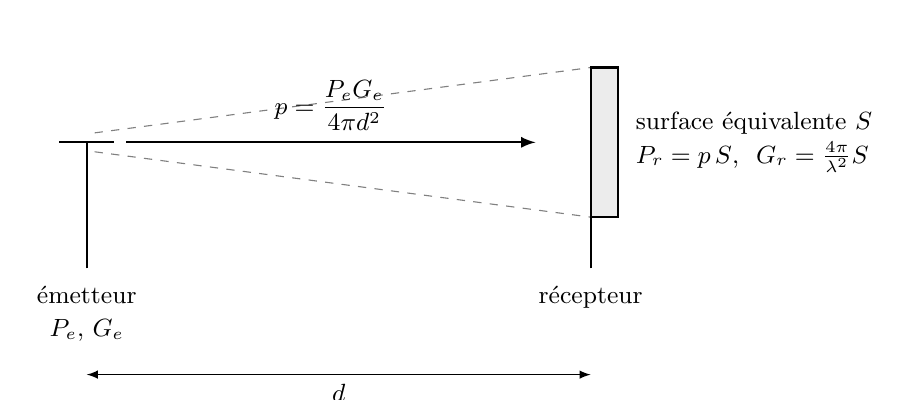
\begin{tikzpicture}[>=latex,scale=1.0]
    % transmitter
    \draw[thick] (0,0) -- (0,1.6);
    \draw[thick] (-0.35,1.6) -- (0.35,1.6);
    \node[align=center,below] at (0,-0.1) {\small émetteur\\ \small $P_e$, $G_e$};
    % beam
    \draw[gray,dashed] (0.1,1.72) -- (6.4,2.55);
    \draw[gray,dashed] (0.1,1.48) -- (6.4,0.65);
    \draw[->,thick] (0.5,1.6) -- (5.7,1.6);
    \node[above] at (3.1,1.62) {\small $p = \dfrac{P_e G_e}{4\pi d^2}$};
    \draw[<->] (0,-1.35) -- (6.4,-1.35) node[midway,below] {\small $d$};
    % receiver
    \draw[thick] (6.4,0) -- (6.4,1.6);
    \draw[thick,fill=gray!15] (6.4,0.65) rectangle (6.75,2.55);
    \node[right,align=left] at (6.85,1.6) {\small surface équivalente $S$\\ \small $P_r = p\,S$, \ $G_r = \frac{4\pi}{\lambda^2}S$};
    \node[align=center,below] at (6.4,-0.1) {\small récepteur};
  \end{tikzpicture}
\end{figure}

\subsubsection{Bilan de liaison d'un satellite géostationnaire}

\begin{problem}[Bilan de liaison d'un satellite géostationnaire]
  On désire établir une communication entre un satellite, placé en orbite
  géostationnaire à une distance $d = 36\,000$~km de la Terre, au moyen d'un
  signal porteur de fréquence $f = 12$~GHz et de puissance $P_E = 100$~W.
  L'antenne d'émission installée sur le satellite possède un gain
  $G_E = 42$~dB. Le système de réception au sol donne un taux d'erreur binaire
  de $10^{-6}$ si la puissance disponible en son entrée --- c'est-à-dire
  \emph{après} l'antenne de réception --- est égale à
  $P_R = 2 \times 10^{-11}$~W, soit $-107$~dBW. Calculer la surface
  équivalente $\Sigma$ de l'antenne de réception au sol et en déduire le gain
  $G_R$ de cette antenne en dB ; déterminer ensuite en dB l'affaiblissement de
  propagation PL.
\end{problem}

\begin{proof}
  On calcule la puissance isotrope rayonnée équivalente (PIRE) par le
  satellite :
  \[ P_{\mathrm{PIRE}} = P_E G_E = 100 \times 10^{4.2} = 1\,584\,893\ \mathrm{W}
     \equiv 62\ \mathrm{dBW}. \]
  On calcule ensuite la densité de puissance reçue sur terre :
  \[ p = \frac{P_{\mathrm{PIRE}}}{4 \pi d^2}
       = \frac{1\,584\,893}{4 \pi \left(36 \times 10^{6}\right)^{2}}
       = 0.973 \times 10^{-10}\ \mathrm{W/m^2}, \]
  avec $d$ en mètres. La relation permettant de calculer la surface
  équivalente de l'antenne au sol --- the surface needed to collect the target
  power --- est la suivante :
  \[ \Sigma = \frac{P_{\text{récep}}}{p}
     = \frac{2 \times 10^{-11}}{0.973 \times 10^{-10}} = 0.205\ \mathrm{m^2}, \]
  et, avec $\lambda = c/f = 2.5$~cm à $12$~GHz, le gain de l'antenne en
  réception au sol vaut
  \[ G_R = \frac{4\pi}{\lambda^2}\Sigma = 4121, \qquad G_{R,\mathrm{dB}} = 36\ \mathrm{dB}. \]
  En regroupant les termes de $P_R = p \Sigma$, cela donne l'équation de Friis,
  et l'on définit l'affaiblissement de propagation par
  \[ \mathrm{PL}_{\mathrm{dB}} = 20 \log \frac{4 \pi d}{\lambda}
     = 20 \log \frac{4\pi \times 36 \times 10^6}{0.025} \approx 205\ \mathrm{dB}. \qed \]
\end{proof}

\begin{remark}
  The budget closes on itself as a check:
  $P_{R,\mathrm{dBW}} = 20 + 42 + 36 - 205 = -107$~dBW, which is the specified
  sensibilité du récepteur. Note the orders of magnitude: $205$~dB of
  affaiblissement en espace libre against $78$~dB of combined gain of the
  antennes, and a received power of $20$~pW.
\end{remark}

\subsubsection{Propagation en visibilité directe}

Par analogie avec l'optique, on pourrait penser que seule l'absence d'obstacles
sur la ligne de visée séparant des antennes d'émission et de réception est
nécessaire pour assurer une \textbf{visibilité directe} (\textit{line of sight})
et appliquer ainsi la formule de Friis. Mais bien que les ondes lumineuses et
radio soient des ondes électromagnétiques et donc soumises aux mêmes lois
(équations de Maxwell), leurs domaines de fréquence sont très différents et les
phénomènes de diffraction ne présentent pas les mêmes ordres de grandeur. Ainsi,
si un obstacle est situé \emph{à proximité} de la ligne de visée entre deux
antennes, celui-ci va causer une diffraction. L'onde diffractée va
s'additionner ou se soustraire avec l'onde transmise en visibilité directe. Ce
phénomène devient négligeable si l'obstacle ne se trouve pas à l'intérieur d'un
volume délimité par le \textbf{premier ellipsoïde de Fresnel}
(\textit{first Fresnel ellipsoid}). On parle de la \emph{règle du dégagement du
premier ellipsoïde}.

\begin{definition}[Premier ellipsoïde de Fresnel]
  Le premier ellipsoïde de Fresnel est centré sur la ligne de visée directe ;
  les deux antennes $E$ et $R$ en sont les foyers, and it is the volume inside
  which an indirect path differs from the direct path by at most $\lambda/2$.
  At a point splitting the link into $d_1$ and $d_2$, son rayon est défini par
  la formule suivante :
  \[ R_f = \sqrt{\lambda\, \frac{d_1 d_2}{d_1 + d_2}}. \]
  Le premier ellipsoïde délimite l'espace dans lequel la plus grande partie de
  l'énergie se propage. Il doit donc être dégagé de tout obstacle.
\end{definition}

\begin{proof}
  Let $A$ be a point on the ellipsoid at horizontal distances $d_1$ and $d_2$
  from $E$ and $R$, at transverse distance $r$. By definition, on peut écrire
  que $EAR = ER + \lambda/2$ avec $ER = d_1 + d_2$, soit
  \[ \sqrt{d_1^2 + r^2} + \sqrt{d_2^2 + r^2} = d_1 + d_2 + \frac{\lambda}{2}. \]
  Avec l'hypothèse $d_1, d_2 \gg r$, on peut écrire que
  \[ d_1 \sqrt{1 + \frac{r^2}{d_1^2}} + d_2 \sqrt{1 + \frac{r^2}{d_2^2}}
     = d_1 + d_2 + \frac{\lambda}{2}, \]
  et en développant au premier ordre, nous obtenons
  \[ d_1\left(1 + \frac{r^2}{2 d_1^2}\right) + d_2\left(1 + \frac{r^2}{2 d_2^2}\right)
     = d_1 + d_2 + \frac{\lambda}{2}
     \;\Longrightarrow\;
     \frac{r^2}{2}\left(\frac{1}{d_1} + \frac{1}{d_2}\right) = \frac{\lambda}{2}, \]
  d'où la distance $r = \sqrt{\lambda\, d_1 d_2/(d_1+d_2)}$. \qed
\end{proof}

\begin{remark}
  $R_f$ decreases as the frequency rises: plus la fréquence augmente, plus
  l'ellipsoïde se rapproche de la ligne de visée directe (cas de l'optique).
  The radius is largest at mid-span, where $d_1 = d_2 = d/2$ and
  $R_{f,\max} = \frac{1}{2}\sqrt{\lambda d}$.
\end{remark}

\begin{example}[Orders of magnitude]
  Soit deux antennes séparées de $1$~km, avec un obstacle à mi-chemin. À
  $2$~GHz, le dégagement nécessaire autour de la ligne de visée pour assurer la
  condition de visibilité directe est de $6$~m. Liaison TDF à $8$~GHz,
  $d_1 + d_2 = 57.6$~km : $R_{f,\max} = 23.2$~m.
\end{example}

\begin{figure}[h!]
  \centering
  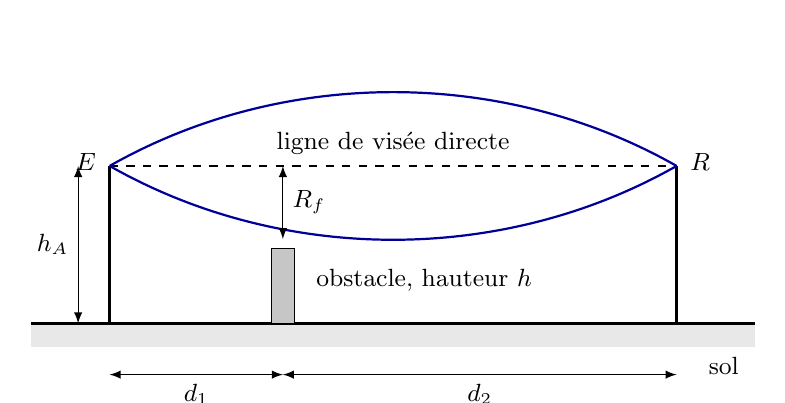
\begin{tikzpicture}[>=latex,scale=1.0]
    \fill[gray!18] (-0.6,-0.3) rectangle (8.6,0);
    \draw[thick] (-0.6,0) -- (8.6,0);
    \node[below] at (8.2,-0.3) {\small sol};
    \draw[very thick] (0.4,0) -- (0.4,2.0);
    \draw[very thick] (7.6,0) -- (7.6,2.0);
    \node[left] at (0.35,2.05) {\small $E$};
    \node[right] at (7.65,2.05) {\small $R$};
    \draw[<->] (0.0,0) -- (0.0,2.0) node[midway,left] {\small $h_A$};
    \draw[thick,dashed] (0.4,2.0) -- (7.6,2.0);
    \node[above] at (4.0,2.02) {\small ligne de visée directe};
    \draw[thick,blue!60!black] (0.4,2.0) .. controls (2.6,3.25) and (5.4,3.25) .. (7.6,2.0);
    \draw[thick,blue!60!black] (0.4,2.0) .. controls (2.6,0.75) and (5.4,0.75) .. (7.6,2.0);
    \draw[<->] (2.6,2.0) -- (2.6,1.07) node[midway,right] {\small $R_f$};
    \draw[fill=gray!45] (2.45,0) rectangle (2.75,0.95);
    \node[right] at (2.9,0.55) {\small obstacle, hauteur $h$};
    \draw[<->] (0.4,-0.65) -- (2.6,-0.65) node[midway,below] {\small $d_1$};
    \draw[<->] (2.6,-0.65) -- (7.6,-0.65) node[midway,below] {\small $d_2$};
  \end{tikzpicture}
\end{figure}

\begin{problem}[Espace dégagé --- ellipsoïde de Fresnel]
  Deux antennes $E$ et $R$, situées à une hauteur $h_A = 20$~m du sol, sont
  séparées d'une distance $d = 10$~km pour lesquelles nous souhaitons établir
  une communication à une fréquence porteuse $f = 2.5$~GHz. On supposera sur
  cette distance que le sol forme un plan.
  \begin{subpart}
    \item Calculer $R_f$ à mi-chemin. Est-ce que la hauteur des antennes est
      suffisante pour que le sol soit en dehors de l'ellipsoïde ?
    \item Un obstacle est situé à $3$~km de l'antenne $E$. Déterminer sa
      hauteur $h$ maximale pour que la liaison soit encore considérée comme
      dégagée.
    \item Dans le cas où il n'y a pas d'obstacle, avec $G_E = G_R = 20$~dB et
      $P_E = 5$~W, calculer la puissance reçue $P_R$.
  \end{subpart}
\end{problem}

\begin{proof}
  À $2.5$~GHz, $\lambda = 12$~cm.\\

  \emph{(a)} Avec $d_1 = d_2 = 5$~km, les dimensions étant en m,
  \[ r = \sqrt{12 \times 10^{-2} \times \frac{25 \times 10^{6}}{10 \times 10^{3}}}
       = \sqrt{300} = 17.3\ \mathrm{m} < h_A = 20\ \mathrm{m}, \]
  donc la hauteur d'antenne est suffisante pour que l'influence du sol sur le
  lien radio soit minimisée. Une hauteur insuffisante occasionnerait des
  phénomènes d'interférences supplémentaires.\\

  \emph{(b)} Avec $d_1 = 3$~km et $d_2 = 7$~km,
  \[ r' = \sqrt{\lambda \frac{d_1 d_2}{d_1+d_2}}
        = \sqrt{12 \times 10^{-2} \times \frac{21 \times 10^{6}}{10^{4}}} = 15.8\ \mathrm{m}, \]
  so the ellipsoid's lower edge is at $h_A - r' = 20 - 15.8 = 4.2$~m. Un
  bâtiment de plus de $4$~m de haut (inférieur à la hauteur d'une maison) sera
  déjà un obstacle non négligeable pour cette liaison malgré un lien en vue
  directe entre les deux antennes.\\

  \emph{(c)} Les gains d'antenne, en échelle linéaire, sont
  $G_E = G_R = 100$ ; $P_E = 5$~W $= 37$~dBm, et
  \[ P_R = P_E G_E G_R \left(\frac{\lambda}{4\pi d}\right)^2
    = 5 \times 100 \times 100 \times \left(\frac{12 \times 10^{-2}}{4\pi \times 10^{4}}\right)^{2}
    \approx 5 \times 10^{-8}\ \mathrm{W}, \]
  ce qui correspond à $-73$~dBW ou $-43$~dBm, which is also read off directly
  as $37 + 20 + 20 - 120$ with $120$~dB of affaiblissement en espace libre.
  \qed
\end{proof}

\subsubsection{Facteurs influençant la propagation}

L'équation de Friis a été obtenue avec l'hypothèse d'une propagation dans le
vide sans obstacles. Or dans la réalité, l'influence de l'environnement sur la
propagation est importante : lors de la propagation, le signal subit de
l'absorption, de la diffraction, des réflexions, de la \textbf{diffusion}
(\textit{scattering}), de la réfraction, etc.

\paragraph{Absorption dans la basse atmosphère} Lors de la propagation d'un
signal dans l'atmosphère, celui-ci subit un affaiblissement linéique (en dB/km)
dû à l'absorption des molécules de dioxygène et des molécules d'eau. Cette
absorption dépend de la fréquence du signal ; on remarque en particulier des
pics d'absorption :

\begin{center}
  \begin{tabular}{@{}ll@{}}
    \toprule
    Molécules & Raies d'absorption \\
    \midrule
    H$_2$O & $22.3$~GHz, $183.3$~GHz, $323$~GHz \\
    O$_2$  & $60$~GHz, $118.74$~GHz \\
    \bottomrule
  \end{tabular}
\end{center}

The reference curve is the affaiblissement linéique par les gaz de
l'atmosphère (ITU-R 719), pression : $1013.6$~mbar, température :
$20\,^\circ$C, vapeur d'eau : $7.5$~g/m$^3$. L'application visée
(communications longue portée ou discrètes) oriente le choix de la fréquence:
the $60$~GHz O$_2$ line is avoided for range and sought, on the contrary, for
deliberately discreet short-range confinement.

\paragraph{Atténuation due à la pluie} La présence de pluie sur une liaison
peut induire une atténuation plus ou moins importante. Two monotonicities hold:
pour une fréquence donnée, plus la pluie est forte, plus l'atténuation est
importante ; pour un taux de pluie donné, l'atténuation augmente avec la
fréquence. Dans les régions tempérées, on considère que la pluie a un effet
significatif au-delà de $5$~GHz, et un effet prépondérant au-delà de $10$~GHz.

\begin{remark}
  L'atténuation due à la pluie se calcule en multipliant l'affaiblissement
  linéique par la \emph{longueur du trajet dans la tranche de pluie}, not by
  the whole link length. It is what fixes the disponibilité de la communication
  en cas de pluie, and therefore the margin that must be carried in the bilan
  de liaison.
\end{remark}

\paragraph{Influence du sol} Le sol est un milieu non magnétique de permittivité
complexe
\[ \bar{\epsilon} = \epsilon - j \frac{\sigma}{\epsilon_0 \omega}. \]
Below a transition frequency the ground behaves as a conducteur, above it as a
diélectrique:
\[ f < f_{\mathrm{transition}} \Rightarrow \text{conducting ground}, \qquad
   f > f_{\mathrm{transition}} \Rightarrow \text{dielectric ground}, \]
avec $f_{\mathrm{transition}} \approx 20$~GHz pour l'eau pure, $\approx 1$~GHz
pour l'eau de mer, et $0.6 - 6$~MHz pour les sols non maritimes. Conséquences
pour un bilan de liaison : prise en compte de l'image de l'antenne (its image
in the ground) ; correction
du facteur de réflexion en fonction de la composition du sol, du relief et de
la distance entre antennes.

\paragraph{Diffraction par le sol} La diffraction par une arête (montagne,
colline) can be computed by treating the obstacle as une arête sans épaisseur.
The practical consequence: sans visibilité directe, on peut tout de même
effectuer une liaison, at the cost of the diffraction loss.

\subsubsection{Milieu réel : modèle de propagation empirique}

Dans le cas d'un environnement complexe (une ville par exemple), où
généralement il n'y a plus de trajet en visibilité directe entre une antenne
d'émission (station de base) et une antenne de réception (smartphone), il est
difficile, voire impossible, de décrire par une relation déterministe
l'atténuation supplémentaire engendrée par le canal de propagation présentant
des trajets multiples (bâtiments, végétation). Pour évaluer l'atténuation dans
ces environnements, la modélisation empirique est utilisée. Les modèles sont
établis à partir de données de mesures d'affaiblissement pour des
environnements types (urbain, suburbain, rural) et utilisables dans de nombreux
cas. Ces modèles permettent aussi bien la planification, en estimant par
simulation l'emplacement optimal d'une station de base dans une cellule, que la
qualification d'un système de communications numériques. De nombreux modèles
d'affaiblissement ont été développés (Hata, Okumura-Hata, 3GPP, Wiener) pour
différents environnements, bandes de fréquence, topographies régionales.

\begin{definition}[Okumura-Hata, rural, $h_m \le 1.5$~m]
  L'influence de la hauteur du mobile étant alors peu significative, le modèle
  d'affaiblissement applicable peut s'écrire
  \begin{align*}
    \mathrm{PL}_{R\text{-}HATA}\,[\mathrm{dB}] =\ & 69.55 + 26.16 \log_{10}(f)
      - 13.82 \log_{10}(h_{bs})
      + \bigl(44.9 - 6.55 \log_{10}(h_{bs})\bigr) \log_{10}(d) \\
      & - 4.78 \left(\log_{10}(f)\right)^{2} + 18.33 \log_{10}(f) - 40.94 .
  \end{align*}
  Les coefficients numériques sont déterminés et tabulés à partir de l'analyse
  des campagnes de mesure effectuées pour chaque type d'environnement.
\end{definition}

\begin{remark}[Units are not SI here]
  Les dimensions des paramètres utilisées dans le modèle de propagation
  Okumura-Hata sont \emph{à conserver telles qu'elles sont} --- the units in
  which the model was fitted: $f$ en MHz, $h_{bs}$ en mètres, $d$ en
  kilomètres. This is the standard trap.
\end{remark}

\begin{problem}[Modèle de propagation empirique]
  Une communication GSM en milieu rural : fréquence $f = 948$~MHz,
  $d = 20$~km, hauteur de la station de base $h_{bs} = 130$~m, hauteur du
  mobile $h_m = 1.5$~m, $G_E = 14$~dB, $G_R = 0$~dB, $P_E = 8$~W. Sur la base
  de la relation
  $P_{R,\mathrm{dBm}} = P_{E,\mathrm{dBm}} + G_{E,\mathrm{dB}} + G_{R,\mathrm{dB}} - L_{\mathrm{dB}}$,
  calculer la puissance $P_R$ disponible au niveau du récepteur du téléphone
  pour le modèle Okumura-Hata et pour le modèle simple de Friis, puis calculer
  la distance $d'$ équivalente avec le modèle de Friis pour la puissance reçue
  obtenue avec le modèle Okumura-Hata.
\end{problem}

\begin{proof}
  Term by term, l'affaiblissement de propagation avec le modèle Okumura-Hata
  rural vaut, avec $f$ en MHz, $h_{bs}$ en m et $d$ en km :
  \[ \mathrm{PL}_{R\text{-}HATA} = 69.55 + 77.87 - 29.2 + 40.36 - 42.35 + 54.56 - 40.94
     \approx 130\ \mathrm{dB}. \]
  Avec $P_E = 8$~W $= 39$~dBm, la puissance reçue vaut
  \[ P_{R,\mathrm{dBm}} = 39 + 14 + 0 - 130 = -77\ \mathrm{dBm}. \]
  Dans le cas de l'application de l'équation de Friis : $\lambda = 0.316$~m,
  $d = 20 \times 10^{3}$~m, et
  \[ \mathrm{PL} = 20 \log_{10}\frac{4 \pi d}{\lambda} = 118\ \mathrm{dB},
     \qquad P_{R,\mathrm{dBm}} = 39 + 14 + 0 - 118 = -65\ \mathrm{dBm}. \]
  Enfin, pour obtenir avec l'équation de Friis le niveau de puissance reçue
  calculé avec le modèle Okumura-Hata,
  \[ 20 \log_{10}\left(\frac{4 \pi d'}{0.316}\right) = 39 + 14 + 77 = 130\ \mathrm{dB}
     \;\Longrightarrow\; d' \approx 78\ \mathrm{km}. \qed \]
\end{proof}

\begin{conclusion}
  The two models disagree by $12$~dB at $20$~km, and translating that gap into
  range turns $20$~km into $78$~km. Ceci indique qu'il est important de faire
  un choix pertinent du modèle d'affaiblissement que l'on utilise pour estimer une
  portée (distance maximale de couverture) lorsque le cahier des charges impose
  un niveau de sensibilité, qui représente la puissance minimale détectable par
  le système de réception pour garantir une qualité de service demandée: that
  level turns directly into a claimed coverage radius, and an optimistic model
  overstates that radius by a factor of four.
\end{conclusion}

\section{Rappel sur les opérateurs vectoriels --- Et pour aller plus loin}
This last chapter does three unrelated jobs. It first collects, as a
reference sheet, les opérateurs différentiels mathématiques appliqués dans un
repère de coordonnées cartésiennes, with which every propagation equation of the
course is written. It then lifts the perfect MLHI hypothesis of Chapter 2 and
lets the medium have losses --- a \textit{diélectrique imparfait} on one side, a
\textit{conducteur imparfait} on the other --- and reads off what the loss does
to the vecteur d'onde and to the fields. It closes by opening onto an area of
current research: the métamatériaux, artificial structures whose permittivité
effective and perméabilité effective take values no natural material offers,
including negative ones.

\begin{notation}
  The operators have a French-style notation,
  $\overrightarrow{\mathrm{grad}}$, $\mathrm{div}$,
  $\overrightarrow{\mathrm{rot}}$, $\Delta$; these notes write $\grad$, $\div$,
  $\curl$ and $\Delta$ for the same four. The cross product is $\wedge$
  throughout, so $\curl\v{F}$ and $\grad\wedge\v{F}$ denote
  the same vector. Vectors are bold: $\v{E}$, $\v{H}$, $\v{F}$, $\v{k}$.\\

  Two collisions of symbols are worth fixing before anything else.
  \begin{subpart}
    \item The \emph{scalar} field of the gradient is written
      $F_{x,y,z}$, meaning $F(x,y,z)$ --- not a component. The components of a
      \emph{vector} field are $F_x$, $F_y$, $F_z$ with a single subscript.
    \item In this chapter $\delta$ is the épaisseur de peau. In Chapter 2 the
      same letter is the angle de perte of the complex permittivité. They are
      different quantities.
  \end{subpart}
  As everywhere in the course the time convention is $e^{+j\omega t}$, so a
  wave travelling towards increasing $z$ carries $e^{j(\omega t - k_z z)}$ and
  the phase spatiale enters with a minus sign.
\end{notation}

\subsection{Définition des opérateurs différentiels utilisés pour la résolution des équations de propagation d'ondes électromagnétiques en coordonnées cartésiennes}

Everything below is stated for a vector field. Soit un vecteur $\v{F}(x,y,z)$
dépendant des variables d'espace définies dans le repère $(O,X,Y,Z)$ :
\[
  \v{F}(x,y,z) = F_x\,\unitv{u}_x + F_y\,\unitv{u}_y + F_z\,\unitv{u}_z ,
\]
où $F_x$, $F_y$, $F_z$ sont les composantes de $\v{F}$ et
$\unitv{u}_x,\unitv{u}_y,\unitv{u}_z$ représentent le système de vecteurs
unitaires associé au repère.
This section is a reference sheet, not a derivation: the six results are used
without further comment in Chapters 2 and 3.

\begin{center}
  \begin{tabular}{llll}
    \toprule
    Operator & French notation & $\grad$ form & Acts on $\to$ gives \\
    \midrule
    nabla & $\vec{\nabla}$ & $\grad$ & --- \\
    gradient & $\overrightarrow{\mathrm{grad}}\,(F_{x,y,z})$ & $\grad F$
      & scalar $\to$ vector \\
    divergence & $\mathrm{div}(\v{F})$ & $\div\v{F}$
      & vector $\to$ scalar \\
    rotationnel & $\overrightarrow{\mathrm{rot}}\,(\v{F})$
      & $\grad\wedge\v{F}$ & vector $\to$ vector \\
    scalar Laplacian & $\Delta(F_x)$ & $\div\grad F_x$
      & scalar $\to$ scalar \\
    vector Laplacian & $\Delta(\v{F})$ & $\grad\cdot\grad\v{F}$
      & vector $\to$ vector \\
    \bottomrule
  \end{tabular}
\end{center}

\paragraph{Nabla.}
C'est l'opérateur différentiel générique qui sert à calculer le gradient, la
divergence, le rotationnel et le Laplacien. It expresses the variation (the
derivative) of a field as a function of its position in space:
\[
  \grad =
  \begin{pmatrix}
    \del/\del x \\[2pt] \del/\del y \\[2pt] \del/\del z
  \end{pmatrix}.
  \tag*{(1)}
\]

\paragraph{Gradient.}
En analyse vectorielle, le gradient est une grandeur \emph{vectorielle}
indiquant la variation d'une grandeur physique dans l'espace. On écrit :
\[
  \overrightarrow{\mathrm{grad}}\,(F_{x,y,z}) =
  \begin{pmatrix}
    \del F_{x,y,z}/\del x \\[2pt]
    \del F_{x,y,z}/\del y \\[2pt]
    \del F_{x,y,z}/\del z
  \end{pmatrix}
  = \grad F_{x,y,z}.
  \tag*{(2)}
\]
Il représente la variation de la valeur du champ \emph{scalaire} dans l'espace.
Colour gradients picture it: a concentric one, whose gradient arrows all point
at the centre, and a unidirectional one, whose arrows are parallel.

\paragraph{Divergence.}
D'une manière générale, la divergence est reliée en physique à l'expression
locale de la propriété de \emph{conservation} d'une grandeur. It turns a vector
field into a scalar; on écrit l'opérateur divergence de cette manière :
\[
  \mathrm{div}(\v{F}) = \frac{\del F_x}{\del x} + \frac{\del F_y}{\del y}
    + \frac{\del F_z}{\del z}.
  \tag*{(3)}
\]

\begin{remark}[Why the MLHI hypothesis saves work]
  Dans le cas d'un MLHI, le milieu est conservateur, dans ce cas
  \[ \div\v{F} = 0 . \]
  Cette propriété permet de simplifier la détermination de l'équation de
  propagation d'une onde électromagnétique dans un MLHI (chapitre 2): it kills
  the $\overrightarrow{\mathrm{grad}}\,(\mathrm{div}(\v{F}))$ term of the
  identity below and leaves a pure Laplacian.
\end{remark}

\paragraph{Rotationnel.}
L'opérateur rotationnel exprime la tendance qu'ont les lignes de champ d'un
champ vectoriel à tourner autour d'un point : sa circulation locale sur un
contour entourant ce point est non nulle quand son rotationnel ne l'est pas.
Par exemple : dans une tornade, le vent tourne autour de l'œil du cyclone et le
champ vectoriel vitesse du vent a un rotationnel non nul autour de l'œil du
cyclone. On développe le calcul ainsi :
\[
  \overrightarrow{\mathrm{rot}}\,(\v{F}) =
  \begin{pmatrix}
    \del F_z/\del y - \del F_y/\del z \\[2pt]
    \del F_x/\del z - \del F_z/\del x \\[2pt]
    \del F_y/\del x - \del F_x/\del y
  \end{pmatrix}
  = \grad \wedge \v{F}
  =
  \begin{pmatrix}
    \del/\del x \\[2pt] \del/\del y \\[2pt] \del/\del z
  \end{pmatrix}
  \wedge
  \begin{pmatrix} F_x \\ F_y \\ F_z \end{pmatrix}.
  \tag*{(4)}
\]
Le rotationnel de $\v{F}$ revient donc à faire le produit vectoriel de
$\grad$ avec $\v{F}$.

\begin{figure}[h!]
  \centering
  \begin{tikzpicture}[>=latex,scale=0.92]
    \draw[gray!50] (0,0) rectangle (3,3);
    \foreach \x in {0.45,1.05,1.65,2.25,2.85}
      \foreach \y in {0.45,1.05,1.65,2.25,2.85}
        \draw[->,thick] (\x-0.20,\y-0.20) -- (\x+0.20,\y+0.20);
    \node at (1.5,-0.5) {a. $\curl\v{F} = \v{0}$};
    \begin{scope}[xshift=4.6cm]
      \draw[gray!50] (0,0) rectangle (3,3);
      \foreach \r in {0.55,1.00,1.35}
        \foreach \t [evaluate=\t as \te using \t+34] in {0,45,...,315}
          \draw[->,thick] ([shift={(\t:\r)}]1.5,1.5)
             -- ([shift={(\te:\r)}]1.5,1.5);
      \node at (1.5,-0.5) {b. $\curl\v{F} \neq \v{0}$};
    \end{scope}
  \end{tikzpicture}
  \caption*{\small Exemple d'interprétation d'un rotationnel appliqué au
  vecteur $\v{F}$. A uniform field circulates to zero on every closed contour;
  a vortex does not.}
\end{figure}

\paragraph{Laplacien vectoriel.}
Le Laplacien vectoriel permet d'estimer la différence entre la valeur de
$\v{F}$ en un point quelconque du milieu et la valeur moyenne de $\v{F}$ au
voisinage de ce point. Component by component, on le définit par :
\[
  \Delta(\v{F}) = \grad\cdot\grad\v{F} =
  \begin{pmatrix}
    \del^2 F_x/\del x^2 + \del^2 F_x/\del y^2 + \del^2 F_x/\del z^2 \\[2pt]
    \del^2 F_y/\del x^2 + \del^2 F_y/\del y^2 + \del^2 F_y/\del z^2 \\[2pt]
    \del^2 F_z/\del x^2 + \del^2 F_z/\del y^2 + \del^2 F_z/\del z^2
  \end{pmatrix}
  =
  \begin{pmatrix} \Delta(F_x) \\ \Delta(F_y) \\ \Delta(F_z) \end{pmatrix}
  =
  \begin{pmatrix}
    \mathrm{div}\big(\overrightarrow{\mathrm{grad}}\,(F_x)\big) \\[2pt]
    \mathrm{div}\big(\overrightarrow{\mathrm{grad}}\,(F_y)\big) \\[2pt]
    \mathrm{div}\big(\overrightarrow{\mathrm{grad}}\,(F_z)\big)
  \end{pmatrix}.
  \tag*{(5)}
\]
The last equality is the definition of the \emph{scalar} Laplacian, which
enters here only implicitly, as $\Delta(F_x) = \mathrm{div}(\overrightarrow{\mathrm{grad}}\,(F_x))$
acting on each cartesian component separately.

\begin{theorem}[Relation fondamentale avec le Laplacien vectoriel]
  \[
    \overrightarrow{\mathrm{rot}}\Big(\overrightarrow{\mathrm{rot}}\,(\v{F})\Big)
    = \overrightarrow{\mathrm{grad}}\Big(\mathrm{div}(\v{F})\Big) - \Delta(\v{F}),
    \qquad\text{i.e.}\qquad
    \curl(\curl\v{F}) = \grad(\div\v{F}) - \Delta(\v{F}).
    \tag*{(6)}
  \]
\end{theorem}

Cette relation est importante pour résoudre les équations de Maxwell: it is
the one result of the section that is used rather than quoted. Taking
the curl of the Maxwell--Faraday equation and substituting Maxwell--Ampère
produces $\curl(\curl\v{E})$; the identity converts it into
$\grad(\div\v{E}) - \Delta(\v{E})$, and in a source-free MLHI the first term
vanishes, leaving the propagation equation solved in Chapter 2.

\begin{remark}
  The simplification of these operators in the particular case of an onde
  plane monochromatique is not carried out in this chapter; it is done where
  it is needed, in Chapter 2, where the wave is taken as
  $e^{j(\omega t - k_z z)}$ so that $\del/\del z$ becomes multiplication by
  $-jk_z$ and the transverse derivatives vanish.
\end{remark}

\subsection{Milieux imparfaits}

Dans le chapitre 2, nous avons présenté le cas de milieux linéaires homogènes
isotropes \emph{parfaits}: a diélectrique of permittivité $\varepsilon$ with
zero conductivité, so that the current density $\v{j}$ in Maxwell--Ampère is
zero and the wave travels without loss. Un \textbf{milieu imparfait}
(\textit{imperfect medium}) présente des pertes. Both cases below --- the
diélectrique imparfait and the conducteur imparfait --- make a non-zero current
density $\v{j}$ appear in the medium; nous présentons ici la conséquence sur
l'expression des champs ainsi que du vecteur d'onde.

\begin{definition}[Les deux régimes]
  Write $\sigma$ for the conductivité of the medium and $\varepsilon$ for its
  permittivité. The medium is treated as
  \begin{subpart}
    \item a \textbf{diélectrique imparfait} (\textit{imperfect dielectric})
      when le diélectrique présente une conductivité $\sigma$ non nulle mais
      $\sigma \ll \omega\varepsilon$;
    \item a \textbf{conducteur imparfait} (\textit{imperfect conductor})
      when, à l'inverse du cas précédent, la conductivité
      $\sigma \gg \omega\varepsilon$.
  \end{subpart}
  The classification is therefore made on the dimensionless ratio
  $\sigma/(\omega\varepsilon)$, and it depends on frequency: the same material
  can be a conducteur at basse fréquence and a diélectrique at high frequency.
\end{definition}

\begin{remark}
  That ratio is the \textbf{tangente de pertes} (\textit{loss tangent})
  $\tan\delta = \varepsilon''/\varepsilon'$ introduced in Chapter 2. The
  derivation below never writes $\tan\delta$ and never names it; it works
  directly with the two inequalities. Remember that $\delta$ in this chapter is
  the épaisseur de peau instead.
\end{remark}

\subsubsection{Cas d'un diélectrique imparfait}

Le diélectrique présente une conductivité $\sigma$ non nulle mais $\sigma \ll
\omega\varepsilon$. L'équation de Maxwell--Ampère s'écrit alors :
\[
  \overrightarrow{\mathrm{rot}}\,\big(\v{H}(z,t)\big)
  = \sigma\v{E}(z,t) + \varepsilon\frac{\del \v{E}(z,t)}{\del t}
  = \sigma\v{E}(z,t) + j\omega\varepsilon\v{E}(z,t)
  = j\omega\varepsilon(\omega)\,\v{E}(z,t),
  \tag*{(7)}
\]
the whole point being that the conduction term and the displacement term can be
merged into a single \emph{complex, frequency-dependent} permittivité
\[
  \varepsilon(\omega) = \varepsilon\left(1 - j\frac{\sigma}{\omega\varepsilon}\right),
  \qquad \varepsilon = \varepsilon_0\varepsilon_r .
\]
The medium is then formally the diélectrique parfait of Chapter 2 with
$\varepsilon$ replaced by $\varepsilon(\omega)$, and all the loss is carried by
the imaginary part.\\

En remplaçant $\varepsilon$ par $\varepsilon(\omega)$, la norme du vecteur
d'onde $\|\v{k}\| = k_z$, pour une OPPM se propageant suivant l'axe $Oz$,
s'écrit :
\[
  k_z^{\,2} = \omega^2\mu_0\varepsilon\left(1 - j\frac{\sigma}{\omega\varepsilon}\right),
  \tag*{(8)}
\]
ce qui donne (since $\sigma \ll \omega\varepsilon$ permits a first-order
expansion of the square root) :
\[
  \boxed{\;k_z \approx \omega\sqrt{\mu_0\varepsilon}
    \left(1 - j\frac{\sigma}{2\omega\varepsilon}\right).\;}
  \tag*{(9)}
\]

Sur l'axe $Oz$, les champs s'écrivent :
\[
  \begin{aligned}
    \v{E}(z,t) &= \v{E}_+(z)\;
      e^{-\sqrt{\mu_0/\varepsilon}\,(\sigma/2)\,z}\;
      e^{\,j(\omega t - \omega\sqrt{\mu_0\varepsilon}\,z)}, \\[2pt]
    \v{H}(z,t) &= \v{H}_+(z)\;
      e^{-\sqrt{\mu_0/\varepsilon}\,(\sigma/2)\,z}\;
      e^{\,j(\omega t - \omega\sqrt{\mu_0\varepsilon}\,z)}.
  \end{aligned}
  \tag*{(10, 11)}
\]

\begin{conclusion}
  Le terme
  $e^{-\sqrt{\mu_0/\varepsilon}\,(\sigma/2)\,z}$ --- a real exponential ---
  correspond à l'atténuation \emph{supplémentaire} de l'onde en fonction de
  $z$ par les pertes du milieu. Reading the two constants off the fields,
  \[
    \alpha = \frac{\sigma}{2}\sqrt{\frac{\mu_0}{\varepsilon}}
    \quad\text{(Np/m)},
    \qquad
    \beta = \omega\sqrt{\mu_0\varepsilon}
    \quad\text{(rad/m)} .
  \]
  To first order the constante de phase is exactly the lossless one of
  Chapter 2: a small conductivité attenuates the wave without changing its
  vitesse de phase.
\end{conclusion}

\subsubsection{Cas d'un conducteur imparfait}

À l'inverse du cas précédent, ici la conductivité $\sigma \gg \omega\varepsilon$:
the displacement term is negligible against the conduction term, and la norme
du vecteur d'onde sera donc égale à :
\[
  k_z^{\,2} \approx -j\omega\mu_0\sigma
  \tag*{(12)}
\]
soit
\[
  k_z \approx \pm\sqrt{\omega\mu_0\sigma}\,\sqrt{-j},
  \qquad \sqrt{-j} = \frac{j-1}{\sqrt{2}} ,
  \tag*{(13)}
\]
et $k_z$ devient :
\[
  k_z \approx \pm\sqrt{\omega\mu_0\sigma}\,\frac{j-1}{\sqrt{2}}
    = \pm\left(j\sqrt{\frac{\omega\mu_0\sigma}{2}} - \sqrt{\frac{\omega\mu_0\sigma}{2}}\right) .
  \tag*{(14)}
\]
Sur l'axe $Oz$, les champs s'écriront :
\[
  \begin{aligned}
    \v{E}(z,t) &= \v{E}_+(z)\;
      e^{-\sqrt{\omega\mu_0\sigma/2}\;z}\;
      e^{\,j\left(\omega t - \sqrt{\omega\mu_0\sigma/2}\;z\right)}, \\[2pt]
    \v{H}(z,t) &= \v{H}_+(z)\;
      e^{-\sqrt{\omega\mu_0\sigma/2}\;z}\;
      e^{\,j\left(\omega t - \sqrt{\omega\mu_0\sigma/2}\;z\right)} .
  \end{aligned}
  \tag*{(15, 16)}
\]

\begin{definition}[Épaisseur de peau (\textit{skin depth})]
  Le terme $\sqrt{\omega\mu_0\sigma/2}$ correspond à un \emph{effet
  pelliculaire}, ce qui indique la présence d'un courant simplement en
  périphérie et non au centre du conducteur. Il s'agit de la définition de la
  pénétration $\delta$ de l'onde dans le conducteur ou autrement appelé
  \textbf{effet de peau} (\textit{skin effect}) :
  \[
    \boxed{\;\delta = \sqrt{\frac{2}{\omega\mu_0\sigma}}\;}
  \]
  Plus la fréquence augmente plus l'épaisseur est fine.
\end{definition}

\begin{remark}[Sign bookkeeping in (14)]
  Both square roots of $-j$ are $\pm(1-j)/\sqrt{2}$, so the $\pm$ in front and
  the choice $\sqrt{-j} = (j-1)/\sqrt{2}$ together do cover the two roots. The
  root actually retained is the one that makes
  (15)--(16) decay towards increasing $z$, namely
  \[
    k_z = \sqrt{\frac{\omega\mu_0\sigma}{2}}\,(1 - j)
        = \frac{1}{\delta} - \frac{j}{\delta} .
  \]
  Read against $e^{j(\omega t - k_z z)}$ this gives $\alpha = \beta = 1/\delta$:
  in a good conducteur the constante d'atténuation and the constante de phase
  are equal. Two consequences worth remembering: the field amplitude falls by a
  factor $e$ over one épaisseur de peau, and the longueur d'onde inside the
  metal is $\lambda = 2\pi/\beta = 2\pi\delta$, so the wave is essentially
  extinguished within a fraction of one internal longueur d'onde.
\end{remark}

\begin{figure}[h!]
  \centering
  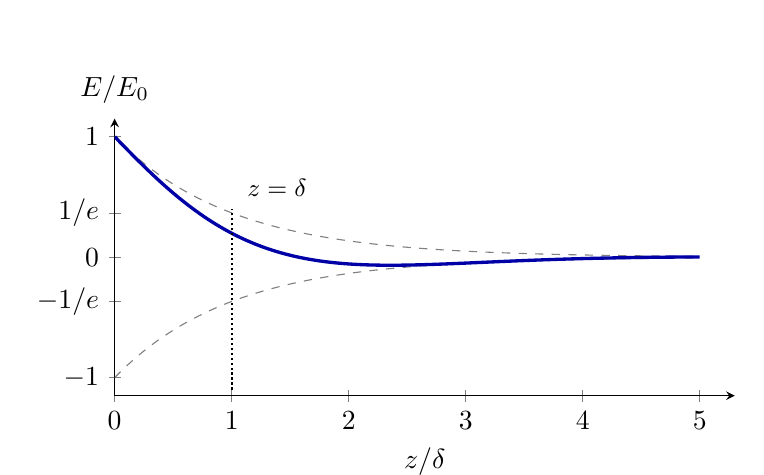
\begin{tikzpicture}
    \begin{axis}[
      width=0.78\textwidth, height=5.1cm,
      xlabel={$z/\delta$}, ylabel={$E/E_0$},
      axis lines=left, domain=0:5, samples=250,
      ymin=-1.15, ymax=1.15, xmin=0, xmax=5.3,
      xtick={0,1,2,3,4,5},
      ytick={-1,-0.368,0,0.368,1},
      yticklabels={$-1$,$-1/e$,$0$,$1/e$,$1$},
      every axis y label/.style={at={(ticklabel* cs:1.02)},anchor=south},
      ]
      \addplot[gray,dashed] {exp(-x)};
      \addplot[gray,dashed] {-exp(-x)};
      \addplot[blue!65!black,very thick] {exp(-x)*cos(deg(x))};
      \draw[densely dotted,thick] (axis cs:1,-1.1) -- (axis cs:1,0.40);
      \node[anchor=south west,font=\small] at (axis cs:1.05,0.42) {$z=\delta$};
    \end{axis}
  \end{tikzpicture}
  \caption*{\small Penetration of the field into a conducteur imparfait. With
  $\alpha = \beta = 1/\delta$ the envelope $e^{-z/\delta}$ and the oscillation
  $\cos(z/\delta)$ share the same scale: one épaisseur de peau costs a factor
  $1/e$ in amplitude and only one radian of phase.}
\end{figure}

\begin{example}[Where the transition sits --- the ground as a lossy medium]
  The ground is treated as a milieu non magnétique de permittivité
  complexe
  \[
    \bar{\epsilon} = \varepsilon - j\frac{\sigma}{\varepsilon_0\omega},
  \]
  and classified by a transition frequency: below $f_{\text{transition}}$
  it is a sol \emph{conducteur}, above it a sol \emph{diélectrique},
  with
  \[
    f_{\text{transition}} \sim 20~\text{GHz (pure water)},\quad
    \sim 1~\text{GHz (sea water)},\quad
    \sim 0.6\text{--}6~\text{MHz (non-maritime soils)} .
  \]
  The practical consequences are the prise en compte de l'image de l'antenne,
  and the correction du facteur de réflexion en fonction de la composition
  du sol, du relief et de la distance entre antennes.
\end{example}

\begin{remark}
  The ground's $\bar{\epsilon}$ and the diélectrique imparfait's
  $\varepsilon(\omega) = \varepsilon - j\sigma/\omega$ differ by a factor
  $\varepsilon_0$. They agree once the $\varepsilon$ of the ground is read as
  the \emph{relative} permittivité: then
  $\bar{\epsilon} = \varepsilon(\omega)/\varepsilon_0$. The criterion
  $\sigma/(\omega\varepsilon)$ is the same in both.
\end{remark}

\subsection{Métamatériaux}

\subsubsection{Introduction}

\begin{definition}[Métamatériau (\textit{metamaterial})]
  En physique, en électromagnétisme, le terme \textbf{métamatériau} sert à
  désigner un matériau \emph{artificiel} qui présente des propriétés
  électromagnétiques qu'on ne retrouve pas dans un matériau naturel. Il s'agit
  généralement de structures \emph{périodiques}, diélectriques ou métalliques,
  qui se comportent comme un matériau homogène n'existant pas à l'état naturel.
\end{definition}

Il existe plusieurs types de métamatériaux en électromagnétisme, les plus
connus étant ceux susceptibles de présenter à la fois une permittivité \emph{et}
une perméabilité négatives. Mais il en existe d'autres : milieux d'impédance
infinis, milieu à permittivité relative inférieure à $1$, etc. Materials are
classified on the quadrant plane $(\Re(\mu), \Re(\varepsilon))$.

\begin{figure}[h!]
  \centering
  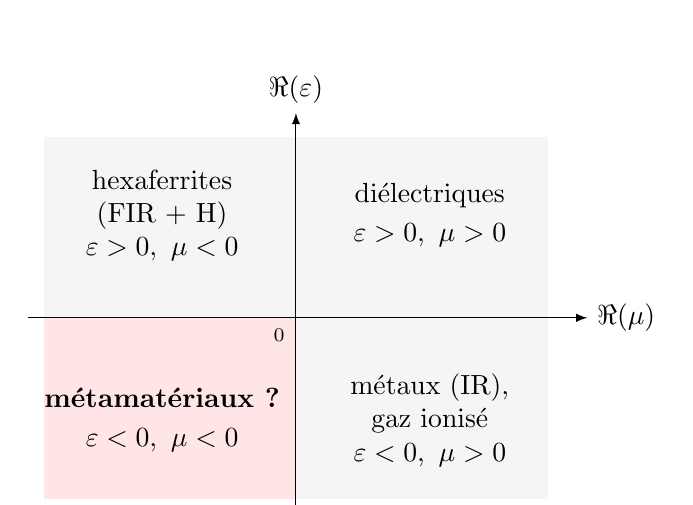
\begin{tikzpicture}[>=latex,scale=1.0]
    \fill[black!4] (-3.2,0) rectangle (3.2,2.3);
    \fill[black!4] (0,-2.3) rectangle (3.2,0);
    \fill[red!10] (-3.2,-2.3) rectangle (0,0);
    \draw[->] (-3.4,0) -- (3.7,0) node[right]{$\Re(\mu)$};
    \draw[->] (0,-2.5) -- (0,2.6) node[above]{$\Re(\varepsilon)$};
    \node[below left,font=\scriptsize] at (-0.02,-0.02) {$0$};
    \node[align=center] at (-1.7,1.3)
      {hexaferrites\\ (FIR + H)\\ $\varepsilon > 0,\ \mu < 0$};
    \node[align=center] at (1.7,1.3)
      {diélectriques\\[2pt] $\varepsilon > 0,\ \mu > 0$};
    \node[align=center] at (1.7,-1.3)
      {métaux (IR),\\ gaz ionisé\\ $\varepsilon < 0,\ \mu > 0$};
    \node[align=center] at (-1.7,-1.3)
      {\textbf{métamatériaux ?}\\[2pt] $\varepsilon < 0,\ \mu < 0$};
  \end{tikzpicture}
  \caption*{\small Classification des matériaux en fonction de leur
  permittivité $\varepsilon$ et perméabilité $\mu$. Three quadrants are
  populated by natural materials; the doubly negative one is the one that has
  to be built.}
\end{figure}

\begin{remark}[ENG and DNG]
  \textbf{ENG} (\textit{epsilon-negative}, $\varepsilon < 0$, $\mu > 0$) and
  \textbf{DNG} (\textit{double-negative}, $\varepsilon < 0$ \emph{and}
  $\mu < 0$) are the literature acronyms for two of the quadrants of the
  classification above, the second being the one labelled « métamatériaux ».
  They are not quadrant labels here --- the classification names its
  quadrants only by material class. They appear only in the subsection on
  antennes below, for the radom material (ENG) and for the double-negative
  material (DNG).
\end{remark}

The stake is not academic. Ces structures trouvent un intérêt remarquable dans
les dispositifs de télécommunications à ondes millimétriques et
submillimétriques qui seront majeurs pour les standards 5G, 6G et au-delà. Ces
ondes trouvent déjà leur place dans divers domaines tels que la spectroscopie,
les applications satellites, les communications, la radioastronomie, etc. The
recurring motivation is \emph{size}: ces activités trouvent leur plein intérêt
dans l'ère du numérique et de l'IoT notamment quand on aborde la réduction de
dimensions souvent liées à la longueur d'onde exploitée dans les systèmes de
communications --- antenne and absorber dimensions are tied to the longueur
d'onde, and a métamatériau lets one keep the performance of a classical system
at a fraction of that size. The other motivation: cela concerne aussi le
domaine de la \textbf{furtivité} (\textit{stealth}) (ou la transparence)
électromagnétique.

\subsubsection{Principe}

Les caractéristiques extraordinaires et même paradoxales des métamatériaux sont
difficiles à réaliser technologiquement et indétectables en pratique dans les
matériaux naturels. Elles sont obtenues grâce aux propriétés du substrat de base
et aux paramètres des cellules unitaires judicieusement sélectionnés. Les
métamatériaux forment alors une large classe de structures composites
constituant des \emph{inclusions} artificielles nommées \textbf{cellules
unitaires} (\textit{unit cells}). Les inclusions ont certaines formes et sont
incorporées dans le milieu de base, généralement un substrat diélectrique ---
for example square metal pads over a plan de masse, connected by vias and
separated by a gap.

\begin{prop}[Homogénéisation]
  La taille (dimensions du « Metal plate ») et la période (dépendante du Gap)
  des cellules unitaires de la plupart des métamatériaux sont \emph{beaucoup
  plus petites que la longueur d'onde opérationnelle}. Par conséquent, un tel
  matériau peut être représenté comme un milieu homogène avec des valeurs
  \emph{effectives} de permittivité et de perméabilité. Ces constantes peuvent
  être modifiées par la manipulation des inclusions individuelles pour obtenir
  les valeurs requises. En d'autres termes, on peut interagir avec les
  ``atomes'' séparés du matériau entier.
\end{prop}

La \textbf{permittivité effective} (\textit{effective permittivity}) et la
\textbf{perméabilité effective} (\textit{effective permeability}) des
composites métamatériaux peuvent prendre des valeurs très grandes ou très
petites, y compris $0$, mais peuvent aussi être \emph{négatives} dans une
certaine bande de fréquence. Dans ce dernier cas, il est possible de réaliser
un milieu à indice de réfraction négatif.

\begin{figure}[h!]
  \centering
  \begin{tikzpicture}[>=latex,scale=0.95]
    % --- panel a : ordinary dielectric, positive refraction
    \begin{scope}
      \fill[blue!4] (-1.9,-1.7) rectangle (1.9,1.5);
      \fill[blue!12] (-1.9,-1.7) rectangle (1.9,0);
      \draw[thick] (-1.9,0) -- (1.9,0);
      \draw[dashed,gray] (0,-1.7) -- (0,1.5);
      \draw[->,thick,blue!60!black] (-1.55,1.35) -- (-0.05,0.03);
      \draw[->,very thick,blue!60!black] (0,0) -- (1.05,-1.6);
      \node[anchor=north west,font=\scriptsize] at (-1.88,-0.05) {diélectrique};
      \node[anchor=south west,font=\scriptsize] at (-1.88,0.05) {diélectrique};
      \node[anchor=west,font=\scriptsize,align=left] at (-1.85,-0.95)
        {$\Re(\varepsilon_r) > 1$\\[1pt] $\v{k}\downarrow$\ \ $\v{\Pi}\downarrow$};
      \node at (0,-2.15) {a. positive refraction};
    \end{scope}
    % --- panel b : metamaterial, negative refraction
    \begin{scope}[xshift=5.6cm]
      \fill[blue!4] (-1.9,-1.7) rectangle (1.9,1.5);
      \fill[red!8] (-1.9,-1.7) rectangle (1.9,0);
      \draw[thick] (-1.9,0) -- (1.9,0);
      \draw[dashed,gray] (0,-1.7) -- (0,1.5);
      \draw[->,thick,red!65!black] (-1.55,1.35) -- (-0.05,0.03);
      \draw[->,very thick,red!65!black] (0,0) -- (-1.15,-1.6);
      \node[anchor=south west,font=\scriptsize] at (-1.88,0.05) {diélectrique};
      \node[anchor=north east,font=\scriptsize] at (1.88,-0.05) {métamatériau};
      \node[anchor=east,font=\scriptsize,align=right] at (1.85,-1.0)
        {$\Re(\varepsilon_r) < 0$\\[1pt] $\v{k}\downarrow$\ \ $\v{\Pi}\uparrow$};
      \node at (0,-2.15) {b. negative refraction};
    \end{scope}
  \end{tikzpicture}
  \caption*{\small Illustration de l'effet d'un indice de réfraction négatif
  matérialisé ici par la partie réelle de la permittivité. In the ordinary
  diélectrique the refracted ray leaves on the far side of the normal and the
  vecteur de Poynting $\v{\Pi}$ follows the vecteur d'onde $\v{k}$; in the
  métamatériau the refracted ray leaves on the \emph{same} side of the normal
  and $\v{\Pi}$ is antiparallel to $\v{k}$.}
\end{figure}

\subsubsection{Permittivité négative}

Les \textbf{fils métalliques minces} (\textit{thin metallic wire}) sont le
premier et le plus connu des matériaux à permittivité négative pour les
applications hyperfréquences. Cette structure a été étudiée par Pendry
\textit{et al.} au milieu des années 90. La structure consiste en une matrice
carrée de fils métalliques minces parallèles et infiniment longs, noyés dans un
milieu diélectrique.

\begin{prop}[Analogie avec le plasma]
  La propagation des ondes électromagnétiques dans une telle structure est
  similaire à la propagation dans un \emph{plasma}. La permittivité du matériau
  composite est négative à la pulsation $\omega < \omega_p$, où $\omega_p$ est
  la pulsation du plasma de la structure. Sa valeur dépend du rayon ($2r$) et de
  la période ($2a$) de placement des fils. La permittivité effective de la
  structure peut s'écrire ainsi :
  \[
    \varepsilon_{\mathit{eff}} = 1 -
      \frac{\omega_p^{\,2}}
           {\omega\left(\omega - j\dfrac{\omega_p^{\,2}a^2\varepsilon_0}{\sigma\pi r^2}\right)},
  \]
  où $r$ est le rayon du fil individuel, $a$ est la période entre les fils
  (avec $r \ll a$) et $\sigma$ la conductivité électrique des fils.
\end{prop}

\begin{figure}[h!]
  \centering
  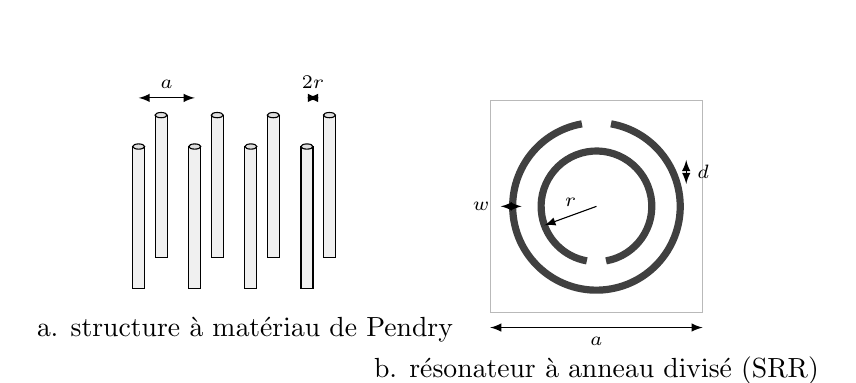
\begin{tikzpicture}[>=latex,scale=0.95]
    % --- (a) Pendry thin-wire medium
    \begin{scope}
      \foreach \i in {0,1,2,3} {
        \foreach \k in {0,1} {
          \pgfmathsetmacro{\xx}{\i*0.75 + \k*0.30}
          \pgfmathsetmacro{\yy}{\k*0.42}
          \draw[fill=gray!12] (\xx,\yy) rectangle (\xx+0.16,\yy+1.9);
          \draw[fill=gray!25] (\xx+0.08,\yy+1.9) ellipse (0.08 and 0.035);
        }
      }
      \draw[<->] (0.08,2.55) -- (0.83,2.55) node[midway,above]{\scriptsize $a$};
      \draw[<->] (2.33,2.55) -- (2.49,2.55) node[midway,above]{\scriptsize $2r$};
      \node at (1.5,-0.55) {a. structure à matériau de Pendry};
    \end{scope}
    % --- (b) circular split-ring resonator
    \begin{scope}[xshift=6.2cm,yshift=1.1cm]
      \draw[gray!55] (-1.42,-1.42) rectangle (1.42,1.42);
      \draw[line width=2.6pt,black!75] (100:1.12) arc (100:440:1.12);
      \draw[line width=2.6pt,black!75] (-80:0.74) arc (-80:260:0.74);
      \draw[<->] (-1.42,-1.62) -- (1.42,-1.62) node[midway,below]{\scriptsize $a$};
      \draw[->] (0,0) -- (200:0.74) node[midway,above]{\scriptsize $r$};
      \draw[<->] (1.2,0.30) -- (1.2,0.62);
      \node[right] at (1.22,0.46) {\scriptsize $d$};
      \draw[<->] (-1.28,0.0) -- (-1.00,0.0);
      \node[left] at (-1.30,0.0) {\scriptsize $w$};
      \node at (0,-2.2) {b. résonateur à anneau divisé (SRR)};
    \end{scope}
  \end{tikzpicture}
  \caption*{\small The two canonical cellules unitaires.
  The wire array gives $\varepsilon_{\mathit{eff}} < 0$ below the plasma
  pulsation; the résonateur à anneau divisé gives $\mu_{\mathit{eff}} < 0$ near
  its resonance.
  $a$ is the cell period, $r$ the inner-ring radius, $d$ the gap between rings,
  $w$ the ring width.}
\end{figure}

La structure tridimensionnelle proposée par Hudlicka est un autre exemple de
structure à permittivité négative à fils. Un treillis de fils connectés à
l'infini forme un élément \emph{triplet}. En utilisant l'approche du milieu
effectif, l'atténuation et les constantes de phase des modes qui se propagent
dans le milieu à triple fil ont été calculées à la fois au-dessous et au-dessus
de la fréquence du plasma. On a découvert que l'onde se propage en dessous de la
fréquence du plasma le long de \emph{toutes} les directions spatiales avec le
même facteur d'atténuation. Ainsi, la triple structure est caractérisée par
l'isotropie par rapport à la direction des ondes électromagnétiques --- which
the planar wire matrix is not.

\subsubsection{Perméabilité négative}

\begin{definition}[Résonateur à anneau divisé (\textit{split-ring resonator}, SRR)]
  La première structure à perméabilité négative, la plus utilisée, est le
  \textbf{résonateur à anneau divisé} (SRR). Les SRR peuvent être à la fois
  géométriquement ronds et carrés et sont caractérisés comme étant une
  structure \emph{résonante} hautement conductrice dans laquelle la capacité
  entre les deux anneaux équilibre l'inductance.
\end{definition}

Un champ magnétique variable dans le temps appliqué perpendiculairement à la
surface des anneaux induit des courants qui produisent le champ magnétique
secondaire. En fonction des propriétés de résonance de la structure, il peut
soit s'opposer au champ incident, soit le renforcer, which results in a
perméabilité effective $\mu_{\mathit{eff}}$ that is positive or negative.

\begin{prop}[Perméabilité effective d'un résonateur circulaire à double anneau fendu]
  Pour un résonateur circulaire, dans le vide, à double anneau fendu (on
  suppose une épaisseur négligeable) :
  \[
    \mu_{\mathit{eff}} = 1 -
      \frac{\pi r^2 / a}
           {1 - \dfrac{3d}{\pi^2\mu_0\varepsilon_0\varepsilon_r^{\,3}}
              + j\dfrac{2\sigma}{\omega\, r\mu_0}} ,
  \]
  où $a$ est la longueur unitaire de la cellule, $d$ est l'intervalle entre les
  anneaux, $r$ est le rayon de l'anneau intérieur et $\sigma$ est la
  conductivité électrique du métal formant l'anneau.
\end{prop}

\begin{remark}
  The formula above is the approximate expression of the perméabilité
  effective, and the narrow frequency band of the first drawback below is the
  one where $\mu_{\mathit{eff}} < 0$ --- that is the property being engineered.
  The secondary magnetic field likewise acts on the perméabilité, not on the
  permittivité: the quantity is $\mu$, never $\varepsilon$, and $\mu$ is the
  relevant quantity throughout the discussion of the SRR.
\end{remark}

\begin{conclusion}[Limits of the first SRRs]
  Les principaux inconvénients des premiers métamatériaux basés sur des
  résonateurs circulaires ou rectangulaires sont
  \begin{subpart}
    \item une bande de fréquence \emph{étroite}, over which the effect exists;
    \item des niveaux élevés de conductivité électrique, required of the metal;
    \item a strong dependence on l'incidence de l'onde éclairant la structure
      --- l'effet de perméabilité négative est observé sous incidence normale ou
      proche de la normale, ce qui réduit fortement le champ d'utilisation.
  \end{subpart}
  Les travaux actuels sont souvent liés à l'augmentation de la bande de
  fréquence ainsi qu'à une incidence d'ondes plus large. Diverses structures ont
  été élaborées sur différentes topologies (2D et 3D) modifiées pour répondre
  aux problèmes --- nested rings, rings loaded with capacitive stubs, tilted
  rings.
\end{conclusion}

\begin{remark}[What made the field famous]
  Ce qui a réellement attiré l'attention sur ces matériaux atypiques a été la
  proposition par J. Pendry de la possibilité de réaliser une
  \textbf{superlentille} (\textit{superlens}) dont la résolution ne serait plus
  limitée par les lois classiques de l'optique. En 2006, J. Pendry et
  U. Leonhardt proposaient la réalisation d'une \textbf{cape d'invisibilité}
  (\textit{invisibility cloak}) utilisant des métamatériaux. Le principe semble
  simple : on utilise un métamatériau dans lequel on fait entrer la lumière, qui
  contourne alors le centre pour reformer l'image initiale intacte de l'autre
  côté. On a alors l'illusion qu'il n'y a rien à l'intérieur du milieu. En
  l'occurrence, le métamatériau n'est pas une cape mais une \emph{sphère} qui
  est utilisée puisqu'elle doit être capable de couvrir tous les angles. Elle
  sera composée de résonateurs disposés sur des cercles concentriques. Ces
  différentes couches se distinguent par leur nombre de charges électriques
  puisque ce sont elles qui vont permettre de guider la lumière à l'intérieur du
  milieu. The demonstration is a cape d'invisibilité hyperfréquence réalisée au
  C2N (ex IEF) à Orsay (équipe André de Lustrac) : une sphère d'invisibilité
  capable de rendre invisible un cylindre d'une vingtaine de centimètres de
  diamètre.
\end{remark}

\subsection{Les métamatériaux dans les systèmes micro-ondes}

Les propriétés électrophysiques particulières des structures artificielles
composites permettent de les utiliser avec succès dans le domaine des
hyperfréquences. La plupart des métamatériaux, tels que les structures à
permittivité, perméabilité ou les 2 négatives sont activement mis en œuvre dans
les guides d'ondes, les résonateurs, les diviseurs de puissance, les
absorbeurs, filtres, coupleurs, isolateurs, antennes et leurs éléments
constructifs. On peut concevoir un guide d'ondes multibande, des réseaux et des
systèmes basés sur les métamatériaux, des composants à bande passante
améliorée, amplificateurs distribués, résonateurs d'ordre zéro, filtres
hyperfréquences avancés, etc.

\subsubsection{Les lignes de propagation}

Les milieux métamatériaux combinés --- negative in permittivité \emph{and} in
perméabilité --- ont trouvé une place dans les systèmes hyperfréquences. On a
découvert que les propriétés électromagnétiques non conventionnelles des
métamatériaux sont observées lorsqu'un matériau est associé avec un autre
matériau ayant au moins une constante matérielle effective de \emph{signe
opposé}.\\

Certaines propriétés sont utilisées sur les lignes de propagation telles que les
guides d'ondes à faces parallèles : en associant différentes couches, il est
possible d'obtenir un mode de propagation TEM avec les propriétés physiques
associées identiques à celles que l'on rencontre en espace libre.\\

Dans les lignes sur substrat, les utilisations de ces types de matériau sont
recherchées aussi, and the sought property is usually phase control. Un exemple
concerne les \textbf{coupleurs} (\textit{couplers}) : un coupleur utilisant une
\textbf{ligne de transmission « main gauche »} (\textit{left-handed line}, LH).

\begin{example}[Coupleur « main gauche »]
  L'ajout d'une structure dite à « main gauche » permet de contrôler la phase
  en sortie de coupleur. On peut obtenir ainsi deux sorties \emph{en phase} sans
  compensation de longueur sur des bandes de fréquence \emph{multiples}. En
  remplaçant les lignes de transmission conventionnelles dans les coupleurs par
  des structures LH, on a fabriqué un coupleur de branche à double bande de
  fréquence : en ajustant la phase en sortie de la ligne de transmission LH, le
  coupleur peut fonctionner à la fréquence fondamentale \emph{et} la première
  harmonique sans changer de structure.
\end{example}

Les coupleurs directionnels basés sur des lignes de transmission à métamatériau
présentent ainsi un couplage amélioré et une gamme de fréquences de
fonctionnement étendue en ayant des dimensions plus compactes par rapport aux
coupleurs conventionnels. Le phénomène de compensation de phase is
characteristic of \textbf{CRLH} (composite right/left-handed) structures. Plus
généralement l'exploitation de ces structures permet d'obtenir des déphaseurs à
large bande avec une erreur de phase faible, des filtres passe-bas et passe-haut
compacts à faibles pertes basés sur l'utilisation de la résonance de la
structure. On y assure de faibles pertes dans la bande et des pertes très
élevées en dehors de la bande tout en conservant une compacité impossible à
atteindre avec une structure traditionnelle.

\subsubsection{Les absorbeurs électromagnétiques micro-ondes}

Une branche particulière des applications est celle des \textbf{absorbeurs
électromagnétiques} (\textit{electromagnetic absorbers}) pour les bandes
hyperfréquences et térahertz. Ils sont constitués d'une couche de métamatériaux et
d'une plaque métallique séparée par un diélectrique; les résonateurs de base et
les dérivés sont largement utilisés comme éléments métamatériaux des absorbeurs
hyperfréquences.

\begin{conclusion}
  Les principaux avantages de ces absorbeurs sont la compacité et la facilité de
  fabrication avec une indépendance vis-à-vis de la polarisation dans une large
  bande de fréquences. Un facteur d'absorption élevé pour de larges angles
  d'incidence et la possibilité de réglage dynamique ont été obtenus.
  L'objectif principal de ces études est de concevoir des absorbeurs
  métamatériaux \emph{parfaits} qui fournissent un facteur d'absorption égal à
  l'unité dans une large gamme d'angles d'incidence et de fréquences. Des
  dispositifs capables d'absorber l'énergie électromagnétique en certains points
  et la transférer en chaleur ont été développés.
\end{conclusion}

Il est possible aussi d'accorder la fréquence de fonctionnement pour les
utiliser comme capteurs sensibles au spectre, notamment dans les
micro-bolomètres, mais l'application principale demeure la réduction de la
\textbf{surface équivalente radar} (\textit{radar cross-section}, SER; RCS in
English) d'un objet fortement réflecteur, comme dans les applications
militaires mais aussi satellites, en minimisant le volume et le poids de cette
structure additionnelle.

\subsubsection{Les antennes}

Dans le cadre de la conception d'antennes, les applications les plus répandues
se focalisent sur les antennes imprimées miniaturisées. Les caractéristiques
d'une antenne sont liées à ses dimensions, aussi réduire la taille d'une
antenne ne doit pas ou peu dégrader les performances nominales. L'une des
approches les plus efficaces pour améliorer le comportement des antennes
\emph{électriquement petites} est de couvrir le ou les éléments rayonnants par
un radom (capot de couverture) à métamatériau dont l'impédance équivalente est
adaptée avec l'espace environnant: for example a monopôle over a plan de masse,
covered by a hemispherical ENG radom of inner radius $r_2$ and outer radius
$r_1$.

\begin{conclusion}[What the radom buys]
  On peut donc réaliser des antennes à haut rendement avec un facteur de
  qualité supérieur en repoussant la limite fondamentale liée à la taille
  physique de l'antenne. Afin de compenser la puissance réactive, on utilise des
  matériaux à permittivité négative (ENG) à forte auto-inductance. En outre,
  l'épaisseur de la couche de métamatériau peut être inférieure au centième de
  la longueur d'onde, ce qui permet d'éviter toute atténuation notable dans ce
  type de système. L'utilisation de matériaux DNG permet d'améliorer la
  conception en réduisant davantage la taille physique et les coûts en
  compensant la puissance rayonnée.
\end{conclusion}

Métamatériaux also go into substrates: l'application dans des \emph{substrats}
pour antennes miniaturisées imprimées permet de réduire la taille des éléments
rayonnants conventionnels, d'augmenter la largeur de bande de l'antenne et
d'améliorer l'efficacité de rayonnement. La structure du substrat est homogène
comme d'habitude et est composée de SRR, d'anneaux chiraux ou de
métasolénoïdes ou en comporte plusieurs types dans une même structure. Il
devient intéressant d'employer les technologies de lignes d'alimentation
« main gauche » pour des antennes réseaux afin de réduire la taille globale de
l'antenne réalisée et de supprimer les interférences des éléments rayonnants
adjacents.\\

Les métamatériaux ont aussi un rôle crucial pour les antennes à réflecteur. On
peut ainsi plaquer l'antenne sur son réflecteur annulant ainsi l'espace entre
les 2, ce qui en réduit le volume global ou, for a mast-mounted antenne, la
prise au vent. À Telecom Paris, une activité reconnue de recherches concerne la
réduction de dimensions des absorbeurs à métamatériau ainsi que celle des
antennes exploitant un \emph{réflecteur magnétique} à métamatériau.

\begin{example}[Réflexion sur un conducteur métallique et sur un conducteur magnétique]
  On place une source d'ondes planes à une hauteur $h < \lambda$ au-dessus
  d'un réflecteur infini ; le réflecteur est modélisé par un facteur de
  réflexion scalaire $\Gamma$, and the quantity sought is le vecteur de
  Poynting résultant de la superposition des ondes directes et réfléchies.\\

  A \emph{metallic} réflecteur has $\Gamma = -1$: the reflected field arrives
  back at the source with a phase $2kh + \pi$, so the two waves add
  constructively in the axis only when $2kh = \pi$, that is
  \[ h = \frac{\lambda}{4}. \]
  The réflecteur must stand a quarter of a longueur d'onde away, which sets the
  usable band and makes the assembly thick.\\

  Un \textbf{conducteur magnétique artificiel} (\textit{artificial magnetic
  conductor}) --- a métamatériau, in contrast --- se caractérise par un
  facteur de réflexion complexe égal à $+1$, ce qui correspond à une
  \emph{impédance de surface infinie}. The reflected field returns in phase for
  $h \to 0$, so the réflecteur can be brought right up against the radiating
  element. That is the advantage of this solution. Deux exemples de plan
  réflecteur magnétique ou métamatériaux (pavage cartésien et concentrique)
  placés en dessous d'une antenne large bande de type spirale d'Archimède
  (antenne bidirectionnelle à polarisation circulaire) : l'objectif est
  d'obtenir une antenne unidirectionnelle (avec un gain augmenté) tout en
  restant mince (ce qu'il est impossible d'obtenir avec un réflecteur
  métallique).
\end{example}

\begin{remark}[References]
  Buriak \textit{et al.}, ``Metamaterials: Theory, Classification and
  Application Strategies'', \textit{J. Nano- Electron. Phys.} \textbf{8}(4)
  (2016), for the survey; Pendry, Holden, Robbins and Stewart, \textit{IEEE
  Trans.\ MTT} (1998), for the medium of fils métalliques minces; Hudlicka,
  Machac and Nefedov,
  \textit{PIER} \textbf{65} (2006), for the 3D triplet lattice; Eleftheriades
  and Balmain, \textit{Negative-refraction Metamaterials} (IEEE--Wiley, 2005),
  for the general theory; and Djoma \textit{et al.}, ``Maximal Bandwidth of an
  Archimedean Spiral Antenna Above a Reflector'', \textit{IEEE AWPL}
  \textbf{13} (2014), for the spiral antenne over a réflecteur of the example
  above.
\end{remark}

\end{document}
